\documentclass[twoside]{book}

% Packages required by doxygen
\usepackage{calc}
\usepackage{doxygen}
\usepackage{graphicx}
\usepackage[utf8]{inputenc}
\usepackage{makeidx}
\usepackage{multicol}
\usepackage{multirow}
\usepackage{textcomp}
\usepackage[table]{xcolor}

% Font selection
\usepackage[T1]{fontenc}
\usepackage{mathptmx}
\usepackage[scaled=.90]{helvet}
\usepackage{courier}
\usepackage{amssymb}
\usepackage{sectsty}
\renewcommand{\familydefault}{\sfdefault}
\allsectionsfont{%
  \fontseries{bc}\selectfont%
  \color{darkgray}%
}
\renewcommand{\DoxyLabelFont}{%
  \fontseries{bc}\selectfont%
  \color{darkgray}%
}

% Page & text layout
\usepackage{geometry}
\geometry{%
  a4paper,%
  top=2.5cm,%
  bottom=2.5cm,%
  left=2.5cm,%
  right=2.5cm%
}
\tolerance=750
\hfuzz=15pt
\hbadness=750
\setlength{\emergencystretch}{15pt}
\setlength{\parindent}{0cm}
\setlength{\parskip}{0.2cm}
\makeatletter
\renewcommand{\paragraph}{%
  \@startsection{paragraph}{4}{0ex}{-1.0ex}{1.0ex}{%
    \normalfont\normalsize\bfseries\SS@parafont%
  }%
}
\renewcommand{\subparagraph}{%
  \@startsection{subparagraph}{5}{0ex}{-1.0ex}{1.0ex}{%
    \normalfont\normalsize\bfseries\SS@subparafont%
  }%
}
\makeatother

% Headers & footers
\usepackage{fancyhdr}
\pagestyle{fancyplain}
\fancyhead[LE]{\fancyplain{}{\bfseries\thepage}}
\fancyhead[CE]{\fancyplain{}{}}
\fancyhead[RE]{\fancyplain{}{\bfseries\leftmark}}
\fancyhead[LO]{\fancyplain{}{\bfseries\rightmark}}
\fancyhead[CO]{\fancyplain{}{}}
\fancyhead[RO]{\fancyplain{}{\bfseries\thepage}}
\fancyfoot[LE]{\fancyplain{}{}}
\fancyfoot[CE]{\fancyplain{}{}}
\fancyfoot[RE]{\fancyplain{}{\bfseries\scriptsize Generated on Mon Jun 26 2017 15\-:16\-:23 for Shine Server by Doxygen }}
\fancyfoot[LO]{\fancyplain{}{\bfseries\scriptsize Generated on Mon Jun 26 2017 15\-:16\-:23 for Shine Server by Doxygen }}
\fancyfoot[CO]{\fancyplain{}{}}
\fancyfoot[RO]{\fancyplain{}{}}
\renewcommand{\footrulewidth}{0.4pt}
\renewcommand{\chaptermark}[1]{%
  \markboth{#1}{}%
}
\renewcommand{\sectionmark}[1]{%
  \markright{\thesection\ #1}%
}

% Indices & bibliography
\usepackage{natbib}
\usepackage[titles]{tocloft}
\setcounter{tocdepth}{3}
\setcounter{secnumdepth}{5}
\makeindex

% Hyperlinks (required, but should be loaded last)
\usepackage{ifpdf}
\ifpdf
  \usepackage[pdftex,pagebackref=true]{hyperref}
\else
  \usepackage[ps2pdf,pagebackref=true]{hyperref}
\fi
\hypersetup{%
  colorlinks=true,%
  linkcolor=blue,%
  citecolor=blue,%
  unicode%
}

% Custom commands
\newcommand{\clearemptydoublepage}{%
  \newpage{\pagestyle{empty}\cleardoublepage}%
}


%===== C O N T E N T S =====

\begin{document}

% Titlepage & ToC
\hypersetup{pageanchor=false}
\pagenumbering{roman}
\begin{titlepage}
\vspace*{7cm}
\begin{center}%
{\Large Shine Server }\\
\vspace*{1cm}
{\large Generated by Doxygen 1.8.6}\\
\vspace*{0.5cm}
{\small Mon Jun 26 2017 15:16:23}\\
\end{center}
\end{titlepage}
\clearemptydoublepage
\tableofcontents
\clearemptydoublepage
\pagenumbering{arabic}
\hypersetup{pageanchor=true}

%--- Begin generated contents ---
\chapter{Class Index}
\section{Class List}
Here are the classes, structs, unions and interfaces with brief descriptions\-:\begin{DoxyCompactList}
\item\contentsline{section}{\hyperlink{structARC__STRUCT}{A\-R\-C\-\_\-\-S\-T\-R\-U\-C\-T} }{\pageref{structARC__STRUCT}}{}
\item\contentsline{section}{\hyperlink{structCF__DATA}{C\-F\-\_\-\-D\-A\-T\-A} }{\pageref{structCF__DATA}}{}
\item\contentsline{section}{\hyperlink{structConfig}{Config} }{\pageref{structConfig}}{}
\item\contentsline{section}{\hyperlink{structDATA__MATRIX}{D\-A\-T\-A\-\_\-\-M\-A\-T\-R\-I\-X} }{\pageref{structDATA__MATRIX}}{}
\item\contentsline{section}{\hyperlink{structHEADER__TRANSMISSION}{H\-E\-A\-D\-E\-R\-\_\-\-T\-R\-A\-N\-S\-M\-I\-S\-S\-I\-O\-N} }{\pageref{structHEADER__TRANSMISSION}}{}
\item\contentsline{section}{\hyperlink{structLIST__STRUCT}{L\-I\-S\-T\-\_\-\-S\-T\-R\-U\-C\-T} }{\pageref{structLIST__STRUCT}}{}
\item\contentsline{section}{\hyperlink{structNODE__LIST__STRUCT}{N\-O\-D\-E\-\_\-\-L\-I\-S\-T\-\_\-\-S\-T\-R\-U\-C\-T} }{\pageref{structNODE__LIST__STRUCT}}{}
\item\contentsline{section}{\hyperlink{structNODE__STRUCT}{N\-O\-D\-E\-\_\-\-S\-T\-R\-U\-C\-T} }{\pageref{structNODE__STRUCT}}{}
\item\contentsline{section}{\hyperlink{structNODE__SUBSET__STRUCT}{N\-O\-D\-E\-\_\-\-S\-U\-B\-S\-E\-T\-\_\-\-S\-T\-R\-U\-C\-T} }{\pageref{structNODE__SUBSET__STRUCT}}{}
\item\contentsline{section}{\hyperlink{structNODO}{N\-O\-D\-O} }{\pageref{structNODO}}{}
\item\contentsline{section}{\hyperlink{structRANDOM__LIST}{R\-A\-N\-D\-O\-M\-\_\-\-L\-I\-S\-T} }{\pageref{structRANDOM__LIST}}{}
\item\contentsline{section}{\hyperlink{structRCL__LIST__STRUCT}{R\-C\-L\-\_\-\-L\-I\-S\-T\-\_\-\-S\-T\-R\-U\-C\-T} }{\pageref{structRCL__LIST__STRUCT}}{}
\item\contentsline{section}{\hyperlink{structSUBSET__STRUCT}{S\-U\-B\-S\-E\-T\-\_\-\-S\-T\-R\-U\-C\-T} }{\pageref{structSUBSET__STRUCT}}{}
\end{DoxyCompactList}

\chapter{File Index}
\section{File List}
Here is a list of all documented files with brief descriptions\-:\begin{DoxyCompactList}
\item\contentsline{section}{\hyperlink{client_8cpp}{client.\-cpp} \\*The main file to use the client }{\pageref{client_8cpp}}{}
\item\contentsline{section}{\hyperlink{CodingDecodingData_8cpp}{Coding\-Decoding\-Data.\-cpp} \\*The file that perform the decoding }{\pageref{CodingDecodingData_8cpp}}{}
\item\contentsline{section}{{\bfseries Coding\-Decoding\-Data.\-h} }{\pageref{CodingDecodingData_8h}}{}
\item\contentsline{section}{{\bfseries Data\-Definition.\-h} }{\pageref{DataDefinition_8h}}{}
\item\contentsline{section}{\hyperlink{LibShine_8cpp}{Lib\-Shine.\-cpp} \\*The file to load configuration file }{\pageref{LibShine_8cpp}}{}
\item\contentsline{section}{{\bfseries Lib\-Shine.\-h} }{\pageref{LibShine_8h}}{}
\item\contentsline{section}{\hyperlink{utilityForTesting_8cpp}{utility\-For\-Testing.\-cpp} \\*A file containing utility function }{\pageref{utilityForTesting_8cpp}}{}
\item\contentsline{section}{{\bfseries utility\-For\-Testing.\-h} }{\pageref{utilityForTesting_8h}}{}
\end{DoxyCompactList}

\chapter{Class Documentation}
\hypertarget{structARC__STRUCT}{\section{A\-R\-C\-\_\-\-S\-T\-R\-U\-C\-T Struct Reference}
\label{structARC__STRUCT}\index{A\-R\-C\-\_\-\-S\-T\-R\-U\-C\-T@{A\-R\-C\-\_\-\-S\-T\-R\-U\-C\-T}}
}


{\ttfamily \#include $<$Data\-Definition.\-h$>$}

\subsection*{Public Attributes}
\begin{DoxyCompactItemize}
\item 
int \hyperlink{structARC__STRUCT_aed399ecc75eab66d87a638f46b12fff1}{adj}
\end{DoxyCompactItemize}


\subsection{Member Data Documentation}
\hypertarget{structARC__STRUCT_aed399ecc75eab66d87a638f46b12fff1}{\index{A\-R\-C\-\_\-\-S\-T\-R\-U\-C\-T@{A\-R\-C\-\_\-\-S\-T\-R\-U\-C\-T}!adj@{adj}}
\index{adj@{adj}!ARC_STRUCT@{A\-R\-C\-\_\-\-S\-T\-R\-U\-C\-T}}
\subsubsection[{adj}]{\setlength{\rightskip}{0pt plus 5cm}int A\-R\-C\-\_\-\-S\-T\-R\-U\-C\-T\-::adj}}\label{structARC__STRUCT_aed399ecc75eab66d87a638f46b12fff1}


The documentation for this struct was generated from the following file\-:\begin{DoxyCompactItemize}
\item 
\hyperlink{DataDefinition_8h}{Data\-Definition.\-h}\end{DoxyCompactItemize}

\hypertarget{structCF__DATA}{\section{C\-F\-\_\-\-D\-A\-T\-A Struct Reference}
\label{structCF__DATA}\index{C\-F\-\_\-\-D\-A\-T\-A@{C\-F\-\_\-\-D\-A\-T\-A}}
}
\subsection*{Public Attributes}
\begin{DoxyCompactItemize}
\item 
\hypertarget{structCF__DATA_a33150ceb864cb8ff1fcf8bfbb2d01efe}{int $\ast$$\ast$ {\bfseries Matrix\-\_\-\-Adj}}\label{structCF__DATA_a33150ceb864cb8ff1fcf8bfbb2d01efe}

\item 
\hypertarget{structCF__DATA_aa790d2fc6304b584e3d6a5afb95cf5c4}{\hyperlink{structNODO}{nodo} $\ast$ {\bfseries nodes}}\label{structCF__DATA_aa790d2fc6304b584e3d6a5afb95cf5c4}

\item 
\hypertarget{structCF__DATA_a50c302ea5a7570881d844eb0b2a6c930}{int {\bfseries n\-\_\-nodi}}\label{structCF__DATA_a50c302ea5a7570881d844eb0b2a6c930}

\item 
\hypertarget{structCF__DATA_a21b2ca110fc0b01950a783ef9e9c2628}{int $\ast$$\ast$$\ast$ {\bfseries Ind}}\label{structCF__DATA_a21b2ca110fc0b01950a783ef9e9c2628}

\end{DoxyCompactItemize}


The documentation for this struct was generated from the following file\-:\begin{DoxyCompactItemize}
\item 
Data\-Definition.\-h\end{DoxyCompactItemize}

\hypertarget{structConfig}{\section{Config Struct Reference}
\label{structConfig}\index{Config@{Config}}
}
\subsection*{Public Attributes}
\begin{DoxyCompactItemize}
\item 
\hypertarget{structConfig_afc8ae6cab0cd9fa1ea54ca13bacd56ea}{int {\bfseries hello\-\_\-port}}\label{structConfig_afc8ae6cab0cd9fa1ea54ca13bacd56ea}

\item 
\hypertarget{structConfig_a2b1264000682b7de201becb6e6fb919d}{char $\ast$ {\bfseries hello\-\_\-group} = new char\mbox{[}10\mbox{]}}\label{structConfig_a2b1264000682b7de201becb6e6fb919d}

\item 
\hypertarget{structConfig_a4a5c2783f6aa2283fb3343082bff5ef7}{int {\bfseries n\-Files}}\label{structConfig_a4a5c2783f6aa2283fb3343082bff5ef7}

\item 
\hypertarget{structConfig_a0a3293605217709540e386fb81eca8bb}{string {\bfseries path\-Repo}}\label{structConfig_a0a3293605217709540e386fb81eca8bb}

\item 
\hypertarget{structConfig_acde368864b2d950bfde458664732a3c6}{int {\bfseries max\-Size}}\label{structConfig_acde368864b2d950bfde458664732a3c6}

\end{DoxyCompactItemize}


The documentation for this struct was generated from the following file\-:\begin{DoxyCompactItemize}
\item 
Lib\-Shine.\-h\end{DoxyCompactItemize}

\hypertarget{structDATA__MATRIX}{\section{D\-A\-T\-A\-\_\-\-M\-A\-T\-R\-I\-X Struct Reference}
\label{structDATA__MATRIX}\index{D\-A\-T\-A\-\_\-\-M\-A\-T\-R\-I\-X@{D\-A\-T\-A\-\_\-\-M\-A\-T\-R\-I\-X}}
}
\subsection*{Public Attributes}
\begin{DoxyCompactItemize}
\item 
\hypertarget{structDATA__MATRIX_aae6daea8805e8718aa68a84bcca6241b}{int {\bfseries n\-\_\-utenti}}\label{structDATA__MATRIX_aae6daea8805e8718aa68a84bcca6241b}

\item 
\hypertarget{structDATA__MATRIX_a4dabab55b019bad68745b2017beca72f}{int {\bfseries m\-\_\-files}}\label{structDATA__MATRIX_a4dabab55b019bad68745b2017beca72f}

\item 
\hypertarget{structDATA__MATRIX_a2d20067a548ed52d36fbc33ea8be6920}{int {\bfseries b\-\_\-chunks}}\label{structDATA__MATRIX_a2d20067a548ed52d36fbc33ea8be6920}

\item 
\hypertarget{structDATA__MATRIX_ab84fa0383965f21e5169de993040734a}{int $\ast$$\ast$$\ast$ {\bfseries Ind}}\label{structDATA__MATRIX_ab84fa0383965f21e5169de993040734a}

\item 
\hypertarget{structDATA__MATRIX_a6cc2252dd6e2e65dd098c0ded22a75a9}{int $\ast$ {\bfseries Q}}\label{structDATA__MATRIX_a6cc2252dd6e2e65dd098c0ded22a75a9}

\item 
\hypertarget{structDATA__MATRIX_afddbea5ee6d0ab5d894b4ac1dc79681c}{int $\ast$$\ast$ {\bfseries Q\-\_\-chuncks}}\label{structDATA__MATRIX_afddbea5ee6d0ab5d894b4ac1dc79681c}

\end{DoxyCompactItemize}


The documentation for this struct was generated from the following file\-:\begin{DoxyCompactItemize}
\item 
Data\-Definition.\-h\end{DoxyCompactItemize}

\hypertarget{structHEADER__TRANSMISSION}{\section{H\-E\-A\-D\-E\-R\-\_\-\-T\-R\-A\-N\-S\-M\-I\-S\-S\-I\-O\-N Struct Reference}
\label{structHEADER__TRANSMISSION}\index{H\-E\-A\-D\-E\-R\-\_\-\-T\-R\-A\-N\-S\-M\-I\-S\-S\-I\-O\-N@{H\-E\-A\-D\-E\-R\-\_\-\-T\-R\-A\-N\-S\-M\-I\-S\-S\-I\-O\-N}}
}


{\ttfamily \#include $<$Data\-Definition.\-h$>$}

\subsection*{Public Attributes}
\begin{DoxyCompactItemize}
\item 
int \hyperlink{structHEADER__TRANSMISSION_a74de1a2343e132bf28eb6e83b4601d34}{padding}
\begin{DoxyCompactList}\small\item\em (1 byte) is used to identify the last chunk for requested file. \end{DoxyCompactList}\item 
int \hyperlink{structHEADER__TRANSMISSION_abee64c077b815db300d99d1e2a273af7}{num\-\_\-chunks}
\begin{DoxyCompactList}\small\item\em define how many chunks are send together. \end{DoxyCompactList}\item 
vector$<$ int $>$ \hyperlink{structHEADER__TRANSMISSION_ae1d8e1fcc8178250b212f77325022424}{id\-\_\-utenti}
\begin{DoxyCompactList}\small\item\em a list of users identifiers. \end{DoxyCompactList}\item 
vector$<$ int $>$ \hyperlink{structHEADER__TRANSMISSION_a7d6396f1a9a35defc1b44e00c663b412}{id\-\_\-files}
\begin{DoxyCompactList}\small\item\em a list of files identifiers. \end{DoxyCompactList}\item 
vector$<$ int $>$ \hyperlink{structHEADER__TRANSMISSION_a3fa5dd88f6fc08f8c64eaee74408ce0e}{id\-\_\-chunks}
\begin{DoxyCompactList}\small\item\em a list of chunks identifiers. \end{DoxyCompactList}\item 
vector$<$ int $>$ \hyperlink{structHEADER__TRANSMISSION_a08672f07c936f6bc4127fe255ea0ce7e}{size\-\_\-package}
\begin{DoxyCompactList}\small\item\em a list of the sizes of every chunk send. This list is useful when padding is 1. \end{DoxyCompactList}\item 
int \hyperlink{structHEADER__TRANSMISSION_a0654a40688064ef0925896891de48b43}{size\-Tot}
\begin{DoxyCompactList}\small\item\em Total package size. \end{DoxyCompactList}\end{DoxyCompactItemize}


\subsection{Member Data Documentation}
\hypertarget{structHEADER__TRANSMISSION_a3fa5dd88f6fc08f8c64eaee74408ce0e}{\index{H\-E\-A\-D\-E\-R\-\_\-\-T\-R\-A\-N\-S\-M\-I\-S\-S\-I\-O\-N@{H\-E\-A\-D\-E\-R\-\_\-\-T\-R\-A\-N\-S\-M\-I\-S\-S\-I\-O\-N}!id\-\_\-chunks@{id\-\_\-chunks}}
\index{id\-\_\-chunks@{id\-\_\-chunks}!HEADER_TRANSMISSION@{H\-E\-A\-D\-E\-R\-\_\-\-T\-R\-A\-N\-S\-M\-I\-S\-S\-I\-O\-N}}
\subsubsection[{id\-\_\-chunks}]{\setlength{\rightskip}{0pt plus 5cm}H\-E\-A\-D\-E\-R\-\_\-\-T\-R\-A\-N\-S\-M\-I\-S\-S\-I\-O\-N\-::id\-\_\-chunks}}\label{structHEADER__TRANSMISSION_a3fa5dd88f6fc08f8c64eaee74408ce0e}


a list of chunks identifiers. 

\hypertarget{structHEADER__TRANSMISSION_a7d6396f1a9a35defc1b44e00c663b412}{\index{H\-E\-A\-D\-E\-R\-\_\-\-T\-R\-A\-N\-S\-M\-I\-S\-S\-I\-O\-N@{H\-E\-A\-D\-E\-R\-\_\-\-T\-R\-A\-N\-S\-M\-I\-S\-S\-I\-O\-N}!id\-\_\-files@{id\-\_\-files}}
\index{id\-\_\-files@{id\-\_\-files}!HEADER_TRANSMISSION@{H\-E\-A\-D\-E\-R\-\_\-\-T\-R\-A\-N\-S\-M\-I\-S\-S\-I\-O\-N}}
\subsubsection[{id\-\_\-files}]{\setlength{\rightskip}{0pt plus 5cm}H\-E\-A\-D\-E\-R\-\_\-\-T\-R\-A\-N\-S\-M\-I\-S\-S\-I\-O\-N\-::id\-\_\-files}}\label{structHEADER__TRANSMISSION_a7d6396f1a9a35defc1b44e00c663b412}


a list of files identifiers. 

\hypertarget{structHEADER__TRANSMISSION_ae1d8e1fcc8178250b212f77325022424}{\index{H\-E\-A\-D\-E\-R\-\_\-\-T\-R\-A\-N\-S\-M\-I\-S\-S\-I\-O\-N@{H\-E\-A\-D\-E\-R\-\_\-\-T\-R\-A\-N\-S\-M\-I\-S\-S\-I\-O\-N}!id\-\_\-utenti@{id\-\_\-utenti}}
\index{id\-\_\-utenti@{id\-\_\-utenti}!HEADER_TRANSMISSION@{H\-E\-A\-D\-E\-R\-\_\-\-T\-R\-A\-N\-S\-M\-I\-S\-S\-I\-O\-N}}
\subsubsection[{id\-\_\-utenti}]{\setlength{\rightskip}{0pt plus 5cm}H\-E\-A\-D\-E\-R\-\_\-\-T\-R\-A\-N\-S\-M\-I\-S\-S\-I\-O\-N\-::id\-\_\-utenti}}\label{structHEADER__TRANSMISSION_ae1d8e1fcc8178250b212f77325022424}


a list of users identifiers. 

\hypertarget{structHEADER__TRANSMISSION_abee64c077b815db300d99d1e2a273af7}{\index{H\-E\-A\-D\-E\-R\-\_\-\-T\-R\-A\-N\-S\-M\-I\-S\-S\-I\-O\-N@{H\-E\-A\-D\-E\-R\-\_\-\-T\-R\-A\-N\-S\-M\-I\-S\-S\-I\-O\-N}!num\-\_\-chunks@{num\-\_\-chunks}}
\index{num\-\_\-chunks@{num\-\_\-chunks}!HEADER_TRANSMISSION@{H\-E\-A\-D\-E\-R\-\_\-\-T\-R\-A\-N\-S\-M\-I\-S\-S\-I\-O\-N}}
\subsubsection[{num\-\_\-chunks}]{\setlength{\rightskip}{0pt plus 5cm}H\-E\-A\-D\-E\-R\-\_\-\-T\-R\-A\-N\-S\-M\-I\-S\-S\-I\-O\-N\-::num\-\_\-chunks}}\label{structHEADER__TRANSMISSION_abee64c077b815db300d99d1e2a273af7}


define how many chunks are send together. 

\hypertarget{structHEADER__TRANSMISSION_a74de1a2343e132bf28eb6e83b4601d34}{\index{H\-E\-A\-D\-E\-R\-\_\-\-T\-R\-A\-N\-S\-M\-I\-S\-S\-I\-O\-N@{H\-E\-A\-D\-E\-R\-\_\-\-T\-R\-A\-N\-S\-M\-I\-S\-S\-I\-O\-N}!padding@{padding}}
\index{padding@{padding}!HEADER_TRANSMISSION@{H\-E\-A\-D\-E\-R\-\_\-\-T\-R\-A\-N\-S\-M\-I\-S\-S\-I\-O\-N}}
\subsubsection[{padding}]{\setlength{\rightskip}{0pt plus 5cm}H\-E\-A\-D\-E\-R\-\_\-\-T\-R\-A\-N\-S\-M\-I\-S\-S\-I\-O\-N\-::padding}}\label{structHEADER__TRANSMISSION_a74de1a2343e132bf28eb6e83b4601d34}


(1 byte) is used to identify the last chunk for requested file. 

\hypertarget{structHEADER__TRANSMISSION_a08672f07c936f6bc4127fe255ea0ce7e}{\index{H\-E\-A\-D\-E\-R\-\_\-\-T\-R\-A\-N\-S\-M\-I\-S\-S\-I\-O\-N@{H\-E\-A\-D\-E\-R\-\_\-\-T\-R\-A\-N\-S\-M\-I\-S\-S\-I\-O\-N}!size\-\_\-package@{size\-\_\-package}}
\index{size\-\_\-package@{size\-\_\-package}!HEADER_TRANSMISSION@{H\-E\-A\-D\-E\-R\-\_\-\-T\-R\-A\-N\-S\-M\-I\-S\-S\-I\-O\-N}}
\subsubsection[{size\-\_\-package}]{\setlength{\rightskip}{0pt plus 5cm}H\-E\-A\-D\-E\-R\-\_\-\-T\-R\-A\-N\-S\-M\-I\-S\-S\-I\-O\-N\-::size\-\_\-package}}\label{structHEADER__TRANSMISSION_a08672f07c936f6bc4127fe255ea0ce7e}


a list of the sizes of every chunk send. This list is useful when padding is 1. 

\hypertarget{structHEADER__TRANSMISSION_a0654a40688064ef0925896891de48b43}{\index{H\-E\-A\-D\-E\-R\-\_\-\-T\-R\-A\-N\-S\-M\-I\-S\-S\-I\-O\-N@{H\-E\-A\-D\-E\-R\-\_\-\-T\-R\-A\-N\-S\-M\-I\-S\-S\-I\-O\-N}!size\-Tot@{size\-Tot}}
\index{size\-Tot@{size\-Tot}!HEADER_TRANSMISSION@{H\-E\-A\-D\-E\-R\-\_\-\-T\-R\-A\-N\-S\-M\-I\-S\-S\-I\-O\-N}}
\subsubsection[{size\-Tot}]{\setlength{\rightskip}{0pt plus 5cm}H\-E\-A\-D\-E\-R\-\_\-\-T\-R\-A\-N\-S\-M\-I\-S\-S\-I\-O\-N\-::size\-Tot}}\label{structHEADER__TRANSMISSION_a0654a40688064ef0925896891de48b43}


Total package size. 



The documentation for this struct was generated from the following file\-:\begin{DoxyCompactItemize}
\item 
\hyperlink{DataDefinition_8h}{Data\-Definition.\-h}\end{DoxyCompactItemize}

\hypertarget{structLIST__STRUCT}{\section{L\-I\-S\-T\-\_\-\-S\-T\-R\-U\-C\-T Struct Reference}
\label{structLIST__STRUCT}\index{L\-I\-S\-T\-\_\-\-S\-T\-R\-U\-C\-T@{L\-I\-S\-T\-\_\-\-S\-T\-R\-U\-C\-T}}
}


{\ttfamily \#include $<$Data\-Definition.\-h$>$}



Collaboration diagram for L\-I\-S\-T\-\_\-\-S\-T\-R\-U\-C\-T\-:
\nopagebreak
\begin{figure}[H]
\begin{center}
\leavevmode
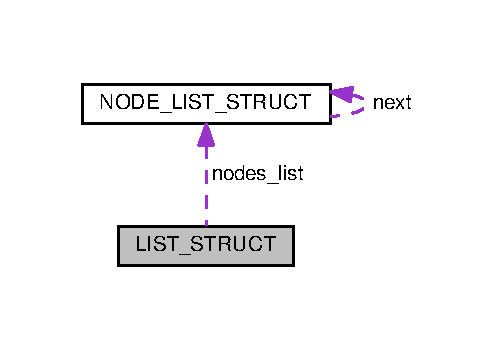
\includegraphics[width=238pt]{structLIST__STRUCT__coll__graph}
\end{center}
\end{figure}
\subsection*{Public Attributes}
\begin{DoxyCompactItemize}
\item 
\hyperlink{DataDefinition_8h_a8804182fdd4652d904801ac03e3d9307}{N\-O\-D\-E\-\_\-\-L\-I\-S\-T} $\ast$ \hyperlink{structLIST__STRUCT_a480f01d85e0c69f63eeeb62c4378e19e}{nodes\-\_\-list}
\end{DoxyCompactItemize}


\subsection{Member Data Documentation}
\hypertarget{structLIST__STRUCT_a480f01d85e0c69f63eeeb62c4378e19e}{\index{L\-I\-S\-T\-\_\-\-S\-T\-R\-U\-C\-T@{L\-I\-S\-T\-\_\-\-S\-T\-R\-U\-C\-T}!nodes\-\_\-list@{nodes\-\_\-list}}
\index{nodes\-\_\-list@{nodes\-\_\-list}!LIST_STRUCT@{L\-I\-S\-T\-\_\-\-S\-T\-R\-U\-C\-T}}
\subsubsection[{nodes\-\_\-list}]{\setlength{\rightskip}{0pt plus 5cm}{\bf N\-O\-D\-E\-\_\-\-L\-I\-S\-T}$\ast$ L\-I\-S\-T\-\_\-\-S\-T\-R\-U\-C\-T\-::nodes\-\_\-list}}\label{structLIST__STRUCT_a480f01d85e0c69f63eeeb62c4378e19e}


The documentation for this struct was generated from the following file\-:\begin{DoxyCompactItemize}
\item 
\hyperlink{DataDefinition_8h}{Data\-Definition.\-h}\end{DoxyCompactItemize}

\hypertarget{structNODE__LIST__STRUCT}{\section{N\-O\-D\-E\-\_\-\-L\-I\-S\-T\-\_\-\-S\-T\-R\-U\-C\-T Struct Reference}
\label{structNODE__LIST__STRUCT}\index{N\-O\-D\-E\-\_\-\-L\-I\-S\-T\-\_\-\-S\-T\-R\-U\-C\-T@{N\-O\-D\-E\-\_\-\-L\-I\-S\-T\-\_\-\-S\-T\-R\-U\-C\-T}}
}


{\ttfamily \#include $<$Data\-Definition.\-h$>$}



Collaboration diagram for N\-O\-D\-E\-\_\-\-L\-I\-S\-T\-\_\-\-S\-T\-R\-U\-C\-T\-:
\nopagebreak
\begin{figure}[H]
\begin{center}
\leavevmode
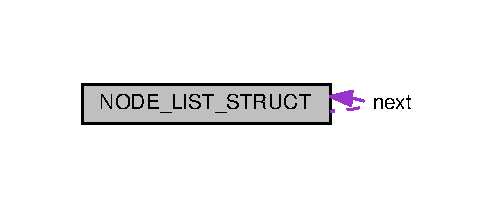
\includegraphics[width=238pt]{structNODE__LIST__STRUCT__coll__graph}
\end{center}
\end{figure}
\subsection*{Public Attributes}
\begin{DoxyCompactItemize}
\item 
int \hyperlink{structNODE__LIST__STRUCT_a34444a74455d1e7d59e13f1dae754321}{id}
\item 
int \hyperlink{structNODE__LIST__STRUCT_a63170b40e99791988837be24d177f65b}{degree}
\item 
int \hyperlink{structNODE__LIST__STRUCT_a5887adfa6a4a3b94ba786593a12fa7ad}{id\-\_\-utente}
\item 
int \hyperlink{structNODE__LIST__STRUCT_abc43d88cc9b8427972095a4637969389}{id\-\_\-file}
\item 
int \hyperlink{structNODE__LIST__STRUCT_a19a415b69b3c7eb1ddeca6ce76670af9}{id\-\_\-chunck}
\item 
struct \hyperlink{structNODE__LIST__STRUCT}{N\-O\-D\-E\-\_\-\-L\-I\-S\-T\-\_\-\-S\-T\-R\-U\-C\-T} $\ast$ \hyperlink{structNODE__LIST__STRUCT_a16cafa75205cd9acf5039b4502613f1a}{next}
\end{DoxyCompactItemize}


\subsection{Member Data Documentation}
\hypertarget{structNODE__LIST__STRUCT_a63170b40e99791988837be24d177f65b}{\index{N\-O\-D\-E\-\_\-\-L\-I\-S\-T\-\_\-\-S\-T\-R\-U\-C\-T@{N\-O\-D\-E\-\_\-\-L\-I\-S\-T\-\_\-\-S\-T\-R\-U\-C\-T}!degree@{degree}}
\index{degree@{degree}!NODE_LIST_STRUCT@{N\-O\-D\-E\-\_\-\-L\-I\-S\-T\-\_\-\-S\-T\-R\-U\-C\-T}}
\subsubsection[{degree}]{\setlength{\rightskip}{0pt plus 5cm}int N\-O\-D\-E\-\_\-\-L\-I\-S\-T\-\_\-\-S\-T\-R\-U\-C\-T\-::degree}}\label{structNODE__LIST__STRUCT_a63170b40e99791988837be24d177f65b}
\hypertarget{structNODE__LIST__STRUCT_a34444a74455d1e7d59e13f1dae754321}{\index{N\-O\-D\-E\-\_\-\-L\-I\-S\-T\-\_\-\-S\-T\-R\-U\-C\-T@{N\-O\-D\-E\-\_\-\-L\-I\-S\-T\-\_\-\-S\-T\-R\-U\-C\-T}!id@{id}}
\index{id@{id}!NODE_LIST_STRUCT@{N\-O\-D\-E\-\_\-\-L\-I\-S\-T\-\_\-\-S\-T\-R\-U\-C\-T}}
\subsubsection[{id}]{\setlength{\rightskip}{0pt plus 5cm}int N\-O\-D\-E\-\_\-\-L\-I\-S\-T\-\_\-\-S\-T\-R\-U\-C\-T\-::id}}\label{structNODE__LIST__STRUCT_a34444a74455d1e7d59e13f1dae754321}
\hypertarget{structNODE__LIST__STRUCT_a19a415b69b3c7eb1ddeca6ce76670af9}{\index{N\-O\-D\-E\-\_\-\-L\-I\-S\-T\-\_\-\-S\-T\-R\-U\-C\-T@{N\-O\-D\-E\-\_\-\-L\-I\-S\-T\-\_\-\-S\-T\-R\-U\-C\-T}!id\-\_\-chunck@{id\-\_\-chunck}}
\index{id\-\_\-chunck@{id\-\_\-chunck}!NODE_LIST_STRUCT@{N\-O\-D\-E\-\_\-\-L\-I\-S\-T\-\_\-\-S\-T\-R\-U\-C\-T}}
\subsubsection[{id\-\_\-chunck}]{\setlength{\rightskip}{0pt plus 5cm}int N\-O\-D\-E\-\_\-\-L\-I\-S\-T\-\_\-\-S\-T\-R\-U\-C\-T\-::id\-\_\-chunck}}\label{structNODE__LIST__STRUCT_a19a415b69b3c7eb1ddeca6ce76670af9}
\hypertarget{structNODE__LIST__STRUCT_abc43d88cc9b8427972095a4637969389}{\index{N\-O\-D\-E\-\_\-\-L\-I\-S\-T\-\_\-\-S\-T\-R\-U\-C\-T@{N\-O\-D\-E\-\_\-\-L\-I\-S\-T\-\_\-\-S\-T\-R\-U\-C\-T}!id\-\_\-file@{id\-\_\-file}}
\index{id\-\_\-file@{id\-\_\-file}!NODE_LIST_STRUCT@{N\-O\-D\-E\-\_\-\-L\-I\-S\-T\-\_\-\-S\-T\-R\-U\-C\-T}}
\subsubsection[{id\-\_\-file}]{\setlength{\rightskip}{0pt plus 5cm}int N\-O\-D\-E\-\_\-\-L\-I\-S\-T\-\_\-\-S\-T\-R\-U\-C\-T\-::id\-\_\-file}}\label{structNODE__LIST__STRUCT_abc43d88cc9b8427972095a4637969389}
\hypertarget{structNODE__LIST__STRUCT_a5887adfa6a4a3b94ba786593a12fa7ad}{\index{N\-O\-D\-E\-\_\-\-L\-I\-S\-T\-\_\-\-S\-T\-R\-U\-C\-T@{N\-O\-D\-E\-\_\-\-L\-I\-S\-T\-\_\-\-S\-T\-R\-U\-C\-T}!id\-\_\-utente@{id\-\_\-utente}}
\index{id\-\_\-utente@{id\-\_\-utente}!NODE_LIST_STRUCT@{N\-O\-D\-E\-\_\-\-L\-I\-S\-T\-\_\-\-S\-T\-R\-U\-C\-T}}
\subsubsection[{id\-\_\-utente}]{\setlength{\rightskip}{0pt plus 5cm}int N\-O\-D\-E\-\_\-\-L\-I\-S\-T\-\_\-\-S\-T\-R\-U\-C\-T\-::id\-\_\-utente}}\label{structNODE__LIST__STRUCT_a5887adfa6a4a3b94ba786593a12fa7ad}
\hypertarget{structNODE__LIST__STRUCT_a16cafa75205cd9acf5039b4502613f1a}{\index{N\-O\-D\-E\-\_\-\-L\-I\-S\-T\-\_\-\-S\-T\-R\-U\-C\-T@{N\-O\-D\-E\-\_\-\-L\-I\-S\-T\-\_\-\-S\-T\-R\-U\-C\-T}!next@{next}}
\index{next@{next}!NODE_LIST_STRUCT@{N\-O\-D\-E\-\_\-\-L\-I\-S\-T\-\_\-\-S\-T\-R\-U\-C\-T}}
\subsubsection[{next}]{\setlength{\rightskip}{0pt plus 5cm}struct {\bf N\-O\-D\-E\-\_\-\-L\-I\-S\-T\-\_\-\-S\-T\-R\-U\-C\-T}$\ast$ N\-O\-D\-E\-\_\-\-L\-I\-S\-T\-\_\-\-S\-T\-R\-U\-C\-T\-::next}}\label{structNODE__LIST__STRUCT_a16cafa75205cd9acf5039b4502613f1a}


The documentation for this struct was generated from the following file\-:\begin{DoxyCompactItemize}
\item 
\hyperlink{DataDefinition_8h}{Data\-Definition.\-h}\end{DoxyCompactItemize}

\hypertarget{structNODE__STRUCT}{\section{N\-O\-D\-E\-\_\-\-S\-T\-R\-U\-C\-T Struct Reference}
\label{structNODE__STRUCT}\index{N\-O\-D\-E\-\_\-\-S\-T\-R\-U\-C\-T@{N\-O\-D\-E\-\_\-\-S\-T\-R\-U\-C\-T}}
}


{\ttfamily \#include $<$Data\-Definition.\-h$>$}



Collaboration diagram for N\-O\-D\-E\-\_\-\-S\-T\-R\-U\-C\-T\-:
\nopagebreak
\begin{figure}[H]
\begin{center}
\leavevmode
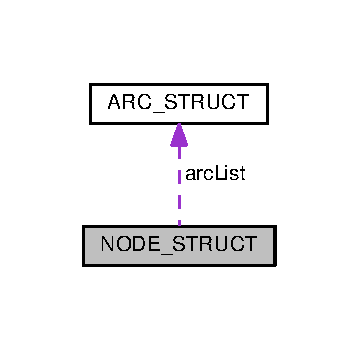
\includegraphics[width=172pt]{structNODE__STRUCT__coll__graph}
\end{center}
\end{figure}
\subsection*{Public Attributes}
\begin{DoxyCompactItemize}
\item 
int \hyperlink{structNODE__STRUCT_a4386a981b07860b03b46d11c5280445d}{id}
\item 
int \hyperlink{structNODE__STRUCT_a4d119525d60341ec5fb1c0f040adb867}{degree}
\item 
struct \hyperlink{structARC__STRUCT}{A\-R\-C\-\_\-\-S\-T\-R\-U\-C\-T} $\ast$ \hyperlink{structNODE__STRUCT_a0a9adf25cd6c875ce28817790e2d93f7}{arc\-List}
\end{DoxyCompactItemize}


\subsection{Member Data Documentation}
\hypertarget{structNODE__STRUCT_a0a9adf25cd6c875ce28817790e2d93f7}{\index{N\-O\-D\-E\-\_\-\-S\-T\-R\-U\-C\-T@{N\-O\-D\-E\-\_\-\-S\-T\-R\-U\-C\-T}!arc\-List@{arc\-List}}
\index{arc\-List@{arc\-List}!NODE_STRUCT@{N\-O\-D\-E\-\_\-\-S\-T\-R\-U\-C\-T}}
\subsubsection[{arc\-List}]{\setlength{\rightskip}{0pt plus 5cm}struct {\bf A\-R\-C\-\_\-\-S\-T\-R\-U\-C\-T}$\ast$ N\-O\-D\-E\-\_\-\-S\-T\-R\-U\-C\-T\-::arc\-List}}\label{structNODE__STRUCT_a0a9adf25cd6c875ce28817790e2d93f7}
\hypertarget{structNODE__STRUCT_a4d119525d60341ec5fb1c0f040adb867}{\index{N\-O\-D\-E\-\_\-\-S\-T\-R\-U\-C\-T@{N\-O\-D\-E\-\_\-\-S\-T\-R\-U\-C\-T}!degree@{degree}}
\index{degree@{degree}!NODE_STRUCT@{N\-O\-D\-E\-\_\-\-S\-T\-R\-U\-C\-T}}
\subsubsection[{degree}]{\setlength{\rightskip}{0pt plus 5cm}int N\-O\-D\-E\-\_\-\-S\-T\-R\-U\-C\-T\-::degree}}\label{structNODE__STRUCT_a4d119525d60341ec5fb1c0f040adb867}
\hypertarget{structNODE__STRUCT_a4386a981b07860b03b46d11c5280445d}{\index{N\-O\-D\-E\-\_\-\-S\-T\-R\-U\-C\-T@{N\-O\-D\-E\-\_\-\-S\-T\-R\-U\-C\-T}!id@{id}}
\index{id@{id}!NODE_STRUCT@{N\-O\-D\-E\-\_\-\-S\-T\-R\-U\-C\-T}}
\subsubsection[{id}]{\setlength{\rightskip}{0pt plus 5cm}int N\-O\-D\-E\-\_\-\-S\-T\-R\-U\-C\-T\-::id}}\label{structNODE__STRUCT_a4386a981b07860b03b46d11c5280445d}


The documentation for this struct was generated from the following file\-:\begin{DoxyCompactItemize}
\item 
\hyperlink{DataDefinition_8h}{Data\-Definition.\-h}\end{DoxyCompactItemize}

\hypertarget{structNODE__SUBSET__STRUCT}{\section{N\-O\-D\-E\-\_\-\-S\-U\-B\-S\-E\-T\-\_\-\-S\-T\-R\-U\-C\-T Struct Reference}
\label{structNODE__SUBSET__STRUCT}\index{N\-O\-D\-E\-\_\-\-S\-U\-B\-S\-E\-T\-\_\-\-S\-T\-R\-U\-C\-T@{N\-O\-D\-E\-\_\-\-S\-U\-B\-S\-E\-T\-\_\-\-S\-T\-R\-U\-C\-T}}
}


{\ttfamily \#include $<$Data\-Definition.\-h$>$}



Collaboration diagram for N\-O\-D\-E\-\_\-\-S\-U\-B\-S\-E\-T\-\_\-\-S\-T\-R\-U\-C\-T\-:
\nopagebreak
\begin{figure}[H]
\begin{center}
\leavevmode
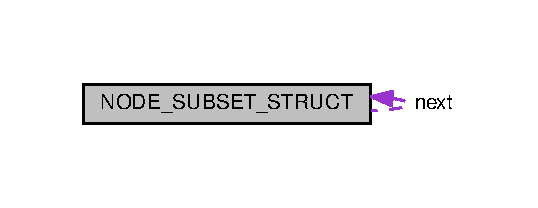
\includegraphics[width=258pt]{structNODE__SUBSET__STRUCT__coll__graph}
\end{center}
\end{figure}
\subsection*{Public Attributes}
\begin{DoxyCompactItemize}
\item 
int \hyperlink{structNODE__SUBSET__STRUCT_a8047d3c37caf8eed1d5cf1db677a6e6a}{id}
\item 
int \hyperlink{structNODE__SUBSET__STRUCT_a8945dd5c7d8177ffbee4acd74ab600d2}{cardinality}
\item 
int $\ast$ \hyperlink{structNODE__SUBSET__STRUCT_a4c704f400a1fa5bb309c1c243422eda1}{label}
\item 
int \hyperlink{structNODE__SUBSET__STRUCT_ab2b2587d1db1672a8dcf6e7050b30f82}{size\-\_\-label}
\item 
struct \hyperlink{structNODE__SUBSET__STRUCT}{N\-O\-D\-E\-\_\-\-S\-U\-B\-S\-E\-T\-\_\-\-S\-T\-R\-U\-C\-T} $\ast$ \hyperlink{structNODE__SUBSET__STRUCT_a23d8738ae1b4513d607523d289e40ace}{next}
\end{DoxyCompactItemize}


\subsection{Member Data Documentation}
\hypertarget{structNODE__SUBSET__STRUCT_a8945dd5c7d8177ffbee4acd74ab600d2}{\index{N\-O\-D\-E\-\_\-\-S\-U\-B\-S\-E\-T\-\_\-\-S\-T\-R\-U\-C\-T@{N\-O\-D\-E\-\_\-\-S\-U\-B\-S\-E\-T\-\_\-\-S\-T\-R\-U\-C\-T}!cardinality@{cardinality}}
\index{cardinality@{cardinality}!NODE_SUBSET_STRUCT@{N\-O\-D\-E\-\_\-\-S\-U\-B\-S\-E\-T\-\_\-\-S\-T\-R\-U\-C\-T}}
\subsubsection[{cardinality}]{\setlength{\rightskip}{0pt plus 5cm}int N\-O\-D\-E\-\_\-\-S\-U\-B\-S\-E\-T\-\_\-\-S\-T\-R\-U\-C\-T\-::cardinality}}\label{structNODE__SUBSET__STRUCT_a8945dd5c7d8177ffbee4acd74ab600d2}
\hypertarget{structNODE__SUBSET__STRUCT_a8047d3c37caf8eed1d5cf1db677a6e6a}{\index{N\-O\-D\-E\-\_\-\-S\-U\-B\-S\-E\-T\-\_\-\-S\-T\-R\-U\-C\-T@{N\-O\-D\-E\-\_\-\-S\-U\-B\-S\-E\-T\-\_\-\-S\-T\-R\-U\-C\-T}!id@{id}}
\index{id@{id}!NODE_SUBSET_STRUCT@{N\-O\-D\-E\-\_\-\-S\-U\-B\-S\-E\-T\-\_\-\-S\-T\-R\-U\-C\-T}}
\subsubsection[{id}]{\setlength{\rightskip}{0pt plus 5cm}int N\-O\-D\-E\-\_\-\-S\-U\-B\-S\-E\-T\-\_\-\-S\-T\-R\-U\-C\-T\-::id}}\label{structNODE__SUBSET__STRUCT_a8047d3c37caf8eed1d5cf1db677a6e6a}
\hypertarget{structNODE__SUBSET__STRUCT_a4c704f400a1fa5bb309c1c243422eda1}{\index{N\-O\-D\-E\-\_\-\-S\-U\-B\-S\-E\-T\-\_\-\-S\-T\-R\-U\-C\-T@{N\-O\-D\-E\-\_\-\-S\-U\-B\-S\-E\-T\-\_\-\-S\-T\-R\-U\-C\-T}!label@{label}}
\index{label@{label}!NODE_SUBSET_STRUCT@{N\-O\-D\-E\-\_\-\-S\-U\-B\-S\-E\-T\-\_\-\-S\-T\-R\-U\-C\-T}}
\subsubsection[{label}]{\setlength{\rightskip}{0pt plus 5cm}int$\ast$ N\-O\-D\-E\-\_\-\-S\-U\-B\-S\-E\-T\-\_\-\-S\-T\-R\-U\-C\-T\-::label}}\label{structNODE__SUBSET__STRUCT_a4c704f400a1fa5bb309c1c243422eda1}
\hypertarget{structNODE__SUBSET__STRUCT_a23d8738ae1b4513d607523d289e40ace}{\index{N\-O\-D\-E\-\_\-\-S\-U\-B\-S\-E\-T\-\_\-\-S\-T\-R\-U\-C\-T@{N\-O\-D\-E\-\_\-\-S\-U\-B\-S\-E\-T\-\_\-\-S\-T\-R\-U\-C\-T}!next@{next}}
\index{next@{next}!NODE_SUBSET_STRUCT@{N\-O\-D\-E\-\_\-\-S\-U\-B\-S\-E\-T\-\_\-\-S\-T\-R\-U\-C\-T}}
\subsubsection[{next}]{\setlength{\rightskip}{0pt plus 5cm}struct {\bf N\-O\-D\-E\-\_\-\-S\-U\-B\-S\-E\-T\-\_\-\-S\-T\-R\-U\-C\-T}$\ast$ N\-O\-D\-E\-\_\-\-S\-U\-B\-S\-E\-T\-\_\-\-S\-T\-R\-U\-C\-T\-::next}}\label{structNODE__SUBSET__STRUCT_a23d8738ae1b4513d607523d289e40ace}
\hypertarget{structNODE__SUBSET__STRUCT_ab2b2587d1db1672a8dcf6e7050b30f82}{\index{N\-O\-D\-E\-\_\-\-S\-U\-B\-S\-E\-T\-\_\-\-S\-T\-R\-U\-C\-T@{N\-O\-D\-E\-\_\-\-S\-U\-B\-S\-E\-T\-\_\-\-S\-T\-R\-U\-C\-T}!size\-\_\-label@{size\-\_\-label}}
\index{size\-\_\-label@{size\-\_\-label}!NODE_SUBSET_STRUCT@{N\-O\-D\-E\-\_\-\-S\-U\-B\-S\-E\-T\-\_\-\-S\-T\-R\-U\-C\-T}}
\subsubsection[{size\-\_\-label}]{\setlength{\rightskip}{0pt plus 5cm}int N\-O\-D\-E\-\_\-\-S\-U\-B\-S\-E\-T\-\_\-\-S\-T\-R\-U\-C\-T\-::size\-\_\-label}}\label{structNODE__SUBSET__STRUCT_ab2b2587d1db1672a8dcf6e7050b30f82}


The documentation for this struct was generated from the following file\-:\begin{DoxyCompactItemize}
\item 
\hyperlink{DataDefinition_8h}{Data\-Definition.\-h}\end{DoxyCompactItemize}

\hypertarget{structNODO}{\section{N\-O\-D\-O Struct Reference}
\label{structNODO}\index{N\-O\-D\-O@{N\-O\-D\-O}}
}
\subsection*{Public Attributes}
\begin{DoxyCompactItemize}
\item 
\hypertarget{structNODO_a363311f2eac0f019bb559decee9d283a}{int {\bfseries id}}\label{structNODO_a363311f2eac0f019bb559decee9d283a}

\item 
\hypertarget{structNODO_ac347f94dfc5042c7a35b5a2ae30796c3}{int {\bfseries degree}}\label{structNODO_ac347f94dfc5042c7a35b5a2ae30796c3}

\item 
\hypertarget{structNODO_a3d58b6fffbdc9fa4dd781d6e5d775ce5}{int {\bfseries id\-\_\-utente}}\label{structNODO_a3d58b6fffbdc9fa4dd781d6e5d775ce5}

\item 
\hypertarget{structNODO_ad1f3355d97fd04e0d908dc196bbf07af}{int {\bfseries id\-\_\-file}}\label{structNODO_ad1f3355d97fd04e0d908dc196bbf07af}

\item 
\hypertarget{structNODO_afff09f10bea60ea56ef2ee708a876017}{int {\bfseries id\-\_\-chunck}}\label{structNODO_afff09f10bea60ea56ef2ee708a876017}

\end{DoxyCompactItemize}


The documentation for this struct was generated from the following file\-:\begin{DoxyCompactItemize}
\item 
Data\-Definition.\-h\end{DoxyCompactItemize}

\hypertarget{structRANDOM__LIST}{\section{R\-A\-N\-D\-O\-M\-\_\-\-L\-I\-S\-T Struct Reference}
\label{structRANDOM__LIST}\index{R\-A\-N\-D\-O\-M\-\_\-\-L\-I\-S\-T@{R\-A\-N\-D\-O\-M\-\_\-\-L\-I\-S\-T}}
}
\subsection*{Public Attributes}
\begin{DoxyCompactItemize}
\item 
\hypertarget{structRANDOM__LIST_a6cd2e0e1e170a5692dc48a4d4c87bdc6}{int {\bfseries idx}}\label{structRANDOM__LIST_a6cd2e0e1e170a5692dc48a4d4c87bdc6}

\item 
\hypertarget{structRANDOM__LIST_a69d18749d83881f09a2742cd6ba19d28}{struct \hyperlink{structRANDOM__LIST}{R\-A\-N\-D\-O\-M\-\_\-\-L\-I\-S\-T} $\ast$ {\bfseries next}}\label{structRANDOM__LIST_a69d18749d83881f09a2742cd6ba19d28}

\end{DoxyCompactItemize}


The documentation for this struct was generated from the following file\-:\begin{DoxyCompactItemize}
\item 
Data\-Definition.\-h\end{DoxyCompactItemize}

\hypertarget{structRCL__LIST__STRUCT}{\section{R\-C\-L\-\_\-\-L\-I\-S\-T\-\_\-\-S\-T\-R\-U\-C\-T Struct Reference}
\label{structRCL__LIST__STRUCT}\index{R\-C\-L\-\_\-\-L\-I\-S\-T\-\_\-\-S\-T\-R\-U\-C\-T@{R\-C\-L\-\_\-\-L\-I\-S\-T\-\_\-\-S\-T\-R\-U\-C\-T}}
}


{\ttfamily \#include $<$Data\-Definition.\-h$>$}

\subsection*{Public Attributes}
\begin{DoxyCompactItemize}
\item 
int \hyperlink{structRCL__LIST__STRUCT_a1fe9da973a851dad04eb6b0272b35adb}{i}
\end{DoxyCompactItemize}


\subsection{Member Data Documentation}
\hypertarget{structRCL__LIST__STRUCT_a1fe9da973a851dad04eb6b0272b35adb}{\index{R\-C\-L\-\_\-\-L\-I\-S\-T\-\_\-\-S\-T\-R\-U\-C\-T@{R\-C\-L\-\_\-\-L\-I\-S\-T\-\_\-\-S\-T\-R\-U\-C\-T}!i@{i}}
\index{i@{i}!RCL_LIST_STRUCT@{R\-C\-L\-\_\-\-L\-I\-S\-T\-\_\-\-S\-T\-R\-U\-C\-T}}
\subsubsection[{i}]{\setlength{\rightskip}{0pt plus 5cm}int R\-C\-L\-\_\-\-L\-I\-S\-T\-\_\-\-S\-T\-R\-U\-C\-T\-::i}}\label{structRCL__LIST__STRUCT_a1fe9da973a851dad04eb6b0272b35adb}


The documentation for this struct was generated from the following file\-:\begin{DoxyCompactItemize}
\item 
\hyperlink{DataDefinition_8h}{Data\-Definition.\-h}\end{DoxyCompactItemize}

\hypertarget{structSUBSET__STRUCT}{\section{S\-U\-B\-S\-E\-T\-\_\-\-S\-T\-R\-U\-C\-T Struct Reference}
\label{structSUBSET__STRUCT}\index{S\-U\-B\-S\-E\-T\-\_\-\-S\-T\-R\-U\-C\-T@{S\-U\-B\-S\-E\-T\-\_\-\-S\-T\-R\-U\-C\-T}}
}
\subsection*{Public Attributes}
\begin{DoxyCompactItemize}
\item 
\hypertarget{structSUBSET__STRUCT_a8023cbde4ffe195b6fa3fd9a7c3211f6}{\hyperlink{structNODE__SUBSET__STRUCT}{N\-O\-D\-E\-\_\-\-S\-U\-B\-S\-E\-T} $\ast$ {\bfseries pt\-\_\-end}}\label{structSUBSET__STRUCT_a8023cbde4ffe195b6fa3fd9a7c3211f6}

\item 
\hypertarget{structSUBSET__STRUCT_a61f3350ae28b746fea56129536e73ec1}{\hyperlink{structNODE__SUBSET__STRUCT}{N\-O\-D\-E\-\_\-\-S\-U\-B\-S\-E\-T} $\ast$ {\bfseries nodes\-\_\-list}}\label{structSUBSET__STRUCT_a61f3350ae28b746fea56129536e73ec1}

\end{DoxyCompactItemize}


The documentation for this struct was generated from the following file\-:\begin{DoxyCompactItemize}
\item 
Data\-Definition.\-h\end{DoxyCompactItemize}

\chapter{File Documentation}
\hypertarget{CheckFunction_8cpp}{\section{Check\-Function.\-cpp File Reference}
\label{CheckFunction_8cpp}\index{Check\-Function.\-cpp@{Check\-Function.\-cpp}}
}


File to check memory allocations.  


{\ttfamily \#include \char`\"{}Check\-Function.\-h\char`\"{}}\\*
Include dependency graph for Check\-Function.\-cpp\-:
\nopagebreak
\begin{figure}[H]
\begin{center}
\leavevmode
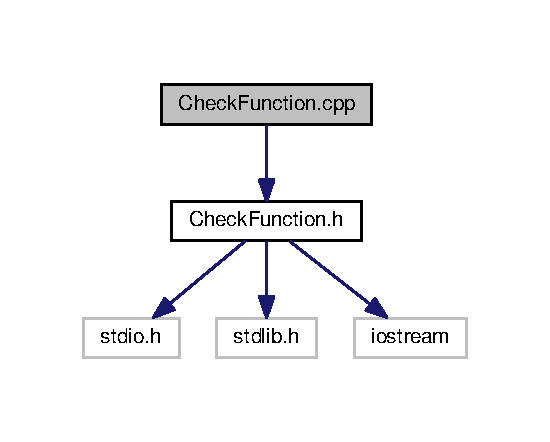
\includegraphics[width=264pt]{CheckFunction_8cpp__incl}
\end{center}
\end{figure}
\subsection*{Functions}
\begin{DoxyCompactItemize}
\item 
void \hyperlink{CheckFunction_8cpp_ad40ce34cc1edd61fbfd997fcf9eaa774}{check\-\_\-memory\-\_\-double\-\_\-allocation\-\_\-1\-D} (double $\ast$pt, string msg)
\item 
void \hyperlink{CheckFunction_8cpp_a60ac9977b6ad887e42be5d608b7c3384}{check\-\_\-memory\-\_\-double\-\_\-allocation\-\_\-2\-D} (double $\ast$$\ast$pt, string msg)
\item 
void \hyperlink{CheckFunction_8cpp_a8f1a46d0330f18cab2b7bf5458a71d03}{check\-\_\-memory\-\_\-allocation\-\_\-1\-D} (int $\ast$pt, string msg)
\item 
void \hyperlink{CheckFunction_8cpp_a12a11983f3c936451eabd25a2f89ceec}{check\-\_\-memory\-\_\-allocation\-\_\-2\-D} (int $\ast$$\ast$pt, string msg)
\item 
void \hyperlink{CheckFunction_8cpp_a917179e80dd117e16637036184490105}{check\-\_\-memory\-\_\-allocation\-\_\-3\-D} (int $\ast$$\ast$$\ast$pt, string msg)
\end{DoxyCompactItemize}
\subsection*{Variables}
\begin{DoxyCompactItemize}
\item 
static const char \hyperlink{CheckFunction_8cpp_a47393496903302e8c659408fe3c651dc}{memory\-\_\-erro} \mbox{[}$\,$\mbox{]} = \char`\"{}\textbackslash{}n\-Error\-: Memory Allocation \-:\char`\"{}
\end{DoxyCompactItemize}


\subsection{Detailed Description}
File to check memory allocations. 

\subsection{Function Documentation}
\hypertarget{CheckFunction_8cpp_a8f1a46d0330f18cab2b7bf5458a71d03}{\index{Check\-Function.\-cpp@{Check\-Function.\-cpp}!check\-\_\-memory\-\_\-allocation\-\_\-1\-D@{check\-\_\-memory\-\_\-allocation\-\_\-1\-D}}
\index{check\-\_\-memory\-\_\-allocation\-\_\-1\-D@{check\-\_\-memory\-\_\-allocation\-\_\-1\-D}!CheckFunction.cpp@{Check\-Function.\-cpp}}
\subsubsection[{check\-\_\-memory\-\_\-allocation\-\_\-1\-D}]{\setlength{\rightskip}{0pt plus 5cm}void check\-\_\-memory\-\_\-allocation\-\_\-1\-D (
\begin{DoxyParamCaption}
\item[{int $\ast$}]{pt, }
\item[{string}]{msg}
\end{DoxyParamCaption}
)}}\label{CheckFunction_8cpp_a8f1a46d0330f18cab2b7bf5458a71d03}


Here is the caller graph for this function\-:
\nopagebreak
\begin{figure}[H]
\begin{center}
\leavevmode
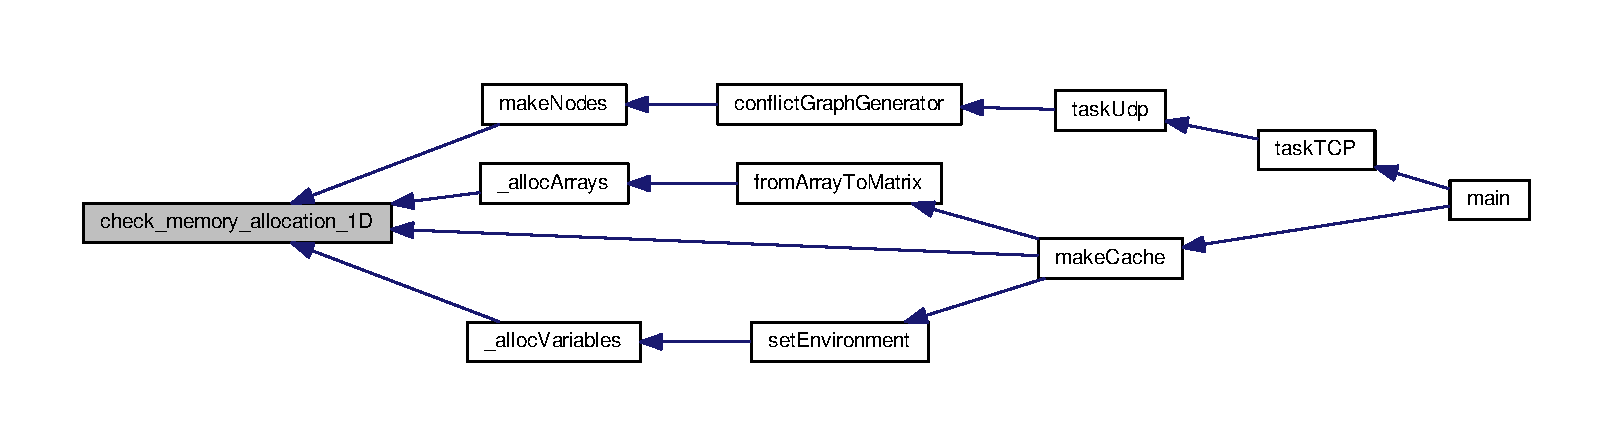
\includegraphics[width=350pt]{CheckFunction_8cpp_a8f1a46d0330f18cab2b7bf5458a71d03_icgraph}
\end{center}
\end{figure}


\hypertarget{CheckFunction_8cpp_a12a11983f3c936451eabd25a2f89ceec}{\index{Check\-Function.\-cpp@{Check\-Function.\-cpp}!check\-\_\-memory\-\_\-allocation\-\_\-2\-D@{check\-\_\-memory\-\_\-allocation\-\_\-2\-D}}
\index{check\-\_\-memory\-\_\-allocation\-\_\-2\-D@{check\-\_\-memory\-\_\-allocation\-\_\-2\-D}!CheckFunction.cpp@{Check\-Function.\-cpp}}
\subsubsection[{check\-\_\-memory\-\_\-allocation\-\_\-2\-D}]{\setlength{\rightskip}{0pt plus 5cm}void check\-\_\-memory\-\_\-allocation\-\_\-2\-D (
\begin{DoxyParamCaption}
\item[{int $\ast$$\ast$}]{pt, }
\item[{string}]{msg}
\end{DoxyParamCaption}
)}}\label{CheckFunction_8cpp_a12a11983f3c936451eabd25a2f89ceec}


Here is the caller graph for this function\-:
\nopagebreak
\begin{figure}[H]
\begin{center}
\leavevmode
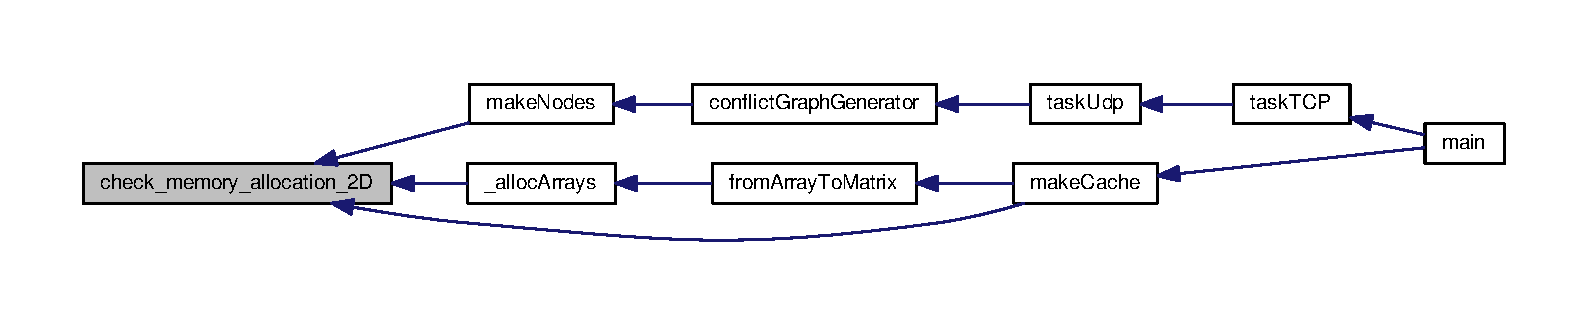
\includegraphics[width=350pt]{CheckFunction_8cpp_a12a11983f3c936451eabd25a2f89ceec_icgraph}
\end{center}
\end{figure}


\hypertarget{CheckFunction_8cpp_a917179e80dd117e16637036184490105}{\index{Check\-Function.\-cpp@{Check\-Function.\-cpp}!check\-\_\-memory\-\_\-allocation\-\_\-3\-D@{check\-\_\-memory\-\_\-allocation\-\_\-3\-D}}
\index{check\-\_\-memory\-\_\-allocation\-\_\-3\-D@{check\-\_\-memory\-\_\-allocation\-\_\-3\-D}!CheckFunction.cpp@{Check\-Function.\-cpp}}
\subsubsection[{check\-\_\-memory\-\_\-allocation\-\_\-3\-D}]{\setlength{\rightskip}{0pt plus 5cm}void check\-\_\-memory\-\_\-allocation\-\_\-3\-D (
\begin{DoxyParamCaption}
\item[{int $\ast$$\ast$$\ast$}]{pt, }
\item[{string}]{msg}
\end{DoxyParamCaption}
)}}\label{CheckFunction_8cpp_a917179e80dd117e16637036184490105}


Here is the caller graph for this function\-:
\nopagebreak
\begin{figure}[H]
\begin{center}
\leavevmode
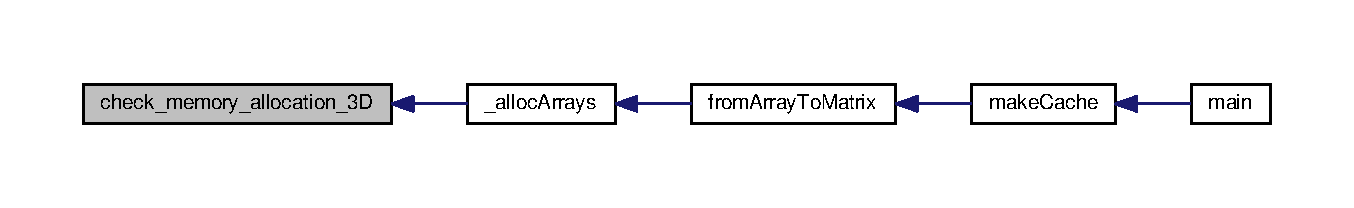
\includegraphics[width=350pt]{CheckFunction_8cpp_a917179e80dd117e16637036184490105_icgraph}
\end{center}
\end{figure}


\hypertarget{CheckFunction_8cpp_ad40ce34cc1edd61fbfd997fcf9eaa774}{\index{Check\-Function.\-cpp@{Check\-Function.\-cpp}!check\-\_\-memory\-\_\-double\-\_\-allocation\-\_\-1\-D@{check\-\_\-memory\-\_\-double\-\_\-allocation\-\_\-1\-D}}
\index{check\-\_\-memory\-\_\-double\-\_\-allocation\-\_\-1\-D@{check\-\_\-memory\-\_\-double\-\_\-allocation\-\_\-1\-D}!CheckFunction.cpp@{Check\-Function.\-cpp}}
\subsubsection[{check\-\_\-memory\-\_\-double\-\_\-allocation\-\_\-1\-D}]{\setlength{\rightskip}{0pt plus 5cm}void check\-\_\-memory\-\_\-double\-\_\-allocation\-\_\-1\-D (
\begin{DoxyParamCaption}
\item[{double $\ast$}]{pt, }
\item[{string}]{msg}
\end{DoxyParamCaption}
)}}\label{CheckFunction_8cpp_ad40ce34cc1edd61fbfd997fcf9eaa774}


Here is the caller graph for this function\-:
\nopagebreak
\begin{figure}[H]
\begin{center}
\leavevmode
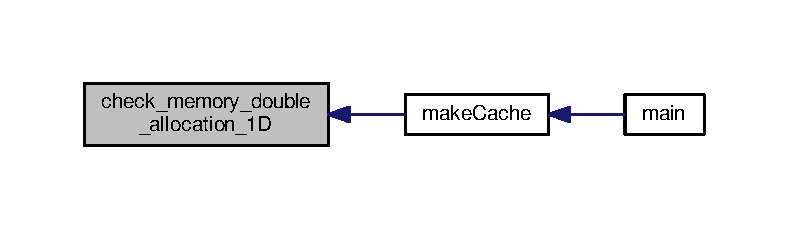
\includegraphics[width=350pt]{CheckFunction_8cpp_ad40ce34cc1edd61fbfd997fcf9eaa774_icgraph}
\end{center}
\end{figure}


\hypertarget{CheckFunction_8cpp_a60ac9977b6ad887e42be5d608b7c3384}{\index{Check\-Function.\-cpp@{Check\-Function.\-cpp}!check\-\_\-memory\-\_\-double\-\_\-allocation\-\_\-2\-D@{check\-\_\-memory\-\_\-double\-\_\-allocation\-\_\-2\-D}}
\index{check\-\_\-memory\-\_\-double\-\_\-allocation\-\_\-2\-D@{check\-\_\-memory\-\_\-double\-\_\-allocation\-\_\-2\-D}!CheckFunction.cpp@{Check\-Function.\-cpp}}
\subsubsection[{check\-\_\-memory\-\_\-double\-\_\-allocation\-\_\-2\-D}]{\setlength{\rightskip}{0pt plus 5cm}void check\-\_\-memory\-\_\-double\-\_\-allocation\-\_\-2\-D (
\begin{DoxyParamCaption}
\item[{double $\ast$$\ast$}]{pt, }
\item[{string}]{msg}
\end{DoxyParamCaption}
)}}\label{CheckFunction_8cpp_a60ac9977b6ad887e42be5d608b7c3384}


Here is the caller graph for this function\-:
\nopagebreak
\begin{figure}[H]
\begin{center}
\leavevmode
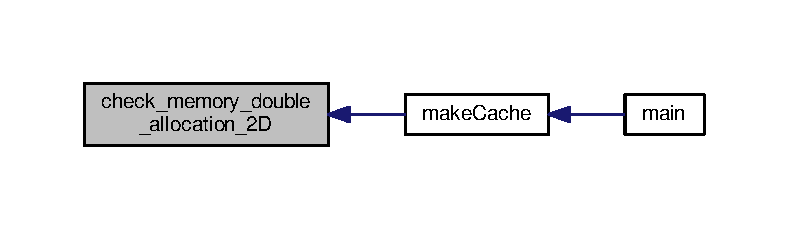
\includegraphics[width=350pt]{CheckFunction_8cpp_a60ac9977b6ad887e42be5d608b7c3384_icgraph}
\end{center}
\end{figure}




\subsection{Variable Documentation}
\hypertarget{CheckFunction_8cpp_a47393496903302e8c659408fe3c651dc}{\index{Check\-Function.\-cpp@{Check\-Function.\-cpp}!memory\-\_\-erro@{memory\-\_\-erro}}
\index{memory\-\_\-erro@{memory\-\_\-erro}!CheckFunction.cpp@{Check\-Function.\-cpp}}
\subsubsection[{memory\-\_\-erro}]{\setlength{\rightskip}{0pt plus 5cm}const char memory\-\_\-erro\mbox{[}$\,$\mbox{]} = \char`\"{}\textbackslash{}n\-Error\-: Memory Allocation \-:\char`\"{}\hspace{0.3cm}{\ttfamily [static]}}}\label{CheckFunction_8cpp_a47393496903302e8c659408fe3c651dc}

\hypertarget{CheckFunction_8h}{\section{Check\-Function.\-h File Reference}
\label{CheckFunction_8h}\index{Check\-Function.\-h@{Check\-Function.\-h}}
}
{\ttfamily \#include $<$stdio.\-h$>$}\\*
{\ttfamily \#include $<$stdlib.\-h$>$}\\*
{\ttfamily \#include $<$iostream$>$}\\*
Include dependency graph for Check\-Function.\-h\-:
\nopagebreak
\begin{figure}[H]
\begin{center}
\leavevmode
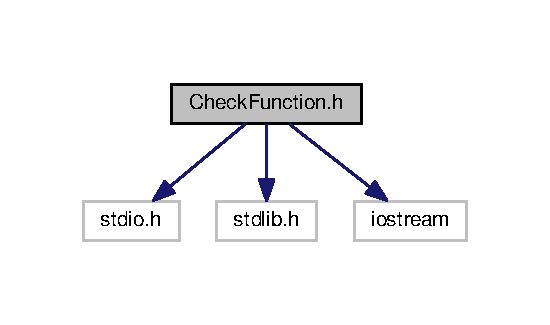
\includegraphics[width=264pt]{CheckFunction_8h__incl}
\end{center}
\end{figure}
This graph shows which files directly or indirectly include this file\-:
\nopagebreak
\begin{figure}[H]
\begin{center}
\leavevmode
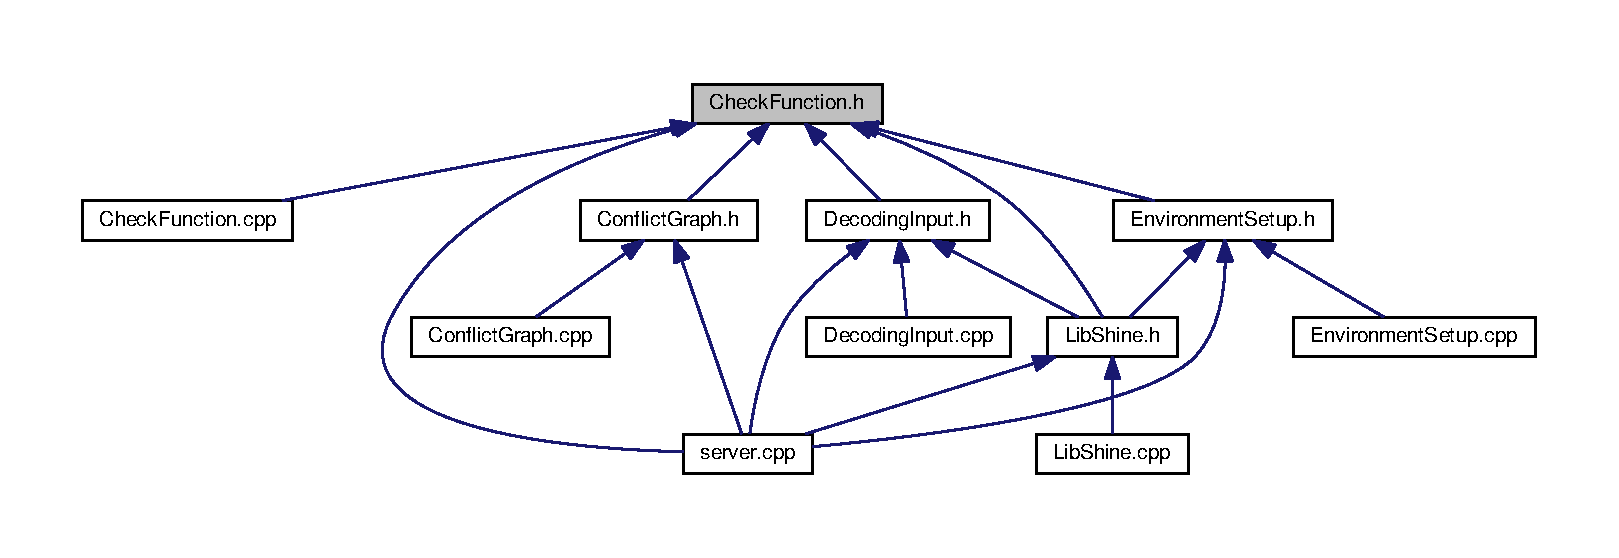
\includegraphics[width=350pt]{CheckFunction_8h__dep__incl}
\end{center}
\end{figure}
\subsection*{Functions}
\begin{DoxyCompactItemize}
\item 
void \hyperlink{CheckFunction_8h_a8f1a46d0330f18cab2b7bf5458a71d03}{check\-\_\-memory\-\_\-allocation\-\_\-1\-D} (int $\ast$pt, string msg)
\item 
void \hyperlink{CheckFunction_8h_a12a11983f3c936451eabd25a2f89ceec}{check\-\_\-memory\-\_\-allocation\-\_\-2\-D} (int $\ast$$\ast$pt, string msg)
\item 
void \hyperlink{CheckFunction_8h_a917179e80dd117e16637036184490105}{check\-\_\-memory\-\_\-allocation\-\_\-3\-D} (int $\ast$$\ast$$\ast$pt, string msg)
\item 
void \hyperlink{CheckFunction_8h_ad40ce34cc1edd61fbfd997fcf9eaa774}{check\-\_\-memory\-\_\-double\-\_\-allocation\-\_\-1\-D} (double $\ast$pt, string msg)
\item 
void \hyperlink{CheckFunction_8h_a60ac9977b6ad887e42be5d608b7c3384}{check\-\_\-memory\-\_\-double\-\_\-allocation\-\_\-2\-D} (double $\ast$$\ast$pt, string msg)
\end{DoxyCompactItemize}


\subsection{Function Documentation}
\hypertarget{CheckFunction_8h_a8f1a46d0330f18cab2b7bf5458a71d03}{\index{Check\-Function.\-h@{Check\-Function.\-h}!check\-\_\-memory\-\_\-allocation\-\_\-1\-D@{check\-\_\-memory\-\_\-allocation\-\_\-1\-D}}
\index{check\-\_\-memory\-\_\-allocation\-\_\-1\-D@{check\-\_\-memory\-\_\-allocation\-\_\-1\-D}!CheckFunction.h@{Check\-Function.\-h}}
\subsubsection[{check\-\_\-memory\-\_\-allocation\-\_\-1\-D}]{\setlength{\rightskip}{0pt plus 5cm}void check\-\_\-memory\-\_\-allocation\-\_\-1\-D (
\begin{DoxyParamCaption}
\item[{int $\ast$}]{pt, }
\item[{string}]{msg}
\end{DoxyParamCaption}
)}}\label{CheckFunction_8h_a8f1a46d0330f18cab2b7bf5458a71d03}


Here is the caller graph for this function\-:
\nopagebreak
\begin{figure}[H]
\begin{center}
\leavevmode
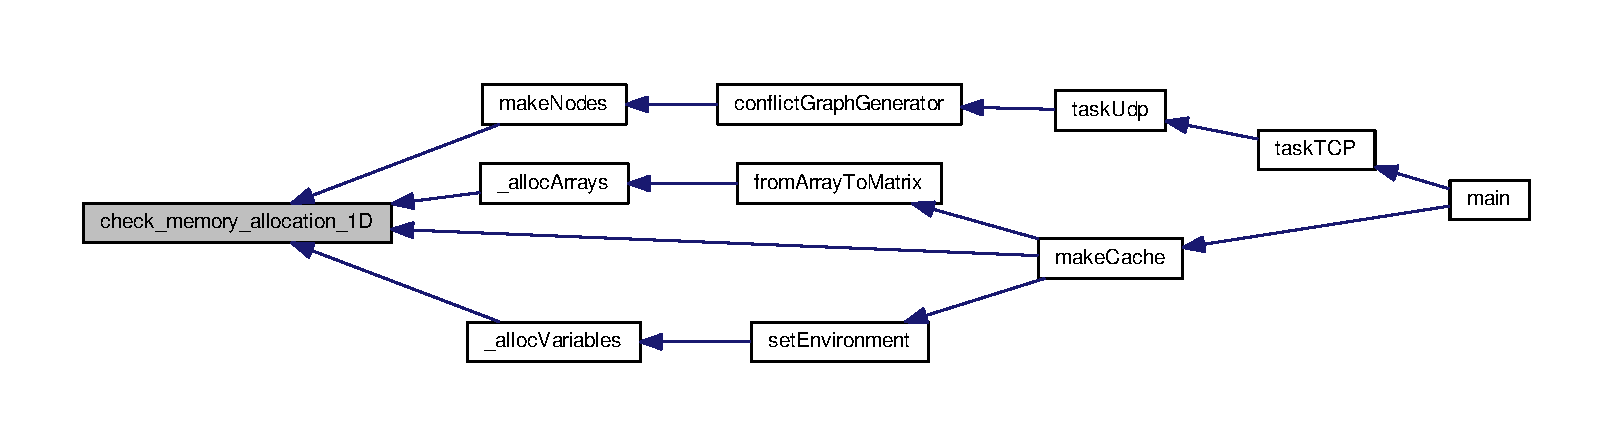
\includegraphics[width=350pt]{CheckFunction_8h_a8f1a46d0330f18cab2b7bf5458a71d03_icgraph}
\end{center}
\end{figure}


\hypertarget{CheckFunction_8h_a12a11983f3c936451eabd25a2f89ceec}{\index{Check\-Function.\-h@{Check\-Function.\-h}!check\-\_\-memory\-\_\-allocation\-\_\-2\-D@{check\-\_\-memory\-\_\-allocation\-\_\-2\-D}}
\index{check\-\_\-memory\-\_\-allocation\-\_\-2\-D@{check\-\_\-memory\-\_\-allocation\-\_\-2\-D}!CheckFunction.h@{Check\-Function.\-h}}
\subsubsection[{check\-\_\-memory\-\_\-allocation\-\_\-2\-D}]{\setlength{\rightskip}{0pt plus 5cm}void check\-\_\-memory\-\_\-allocation\-\_\-2\-D (
\begin{DoxyParamCaption}
\item[{int $\ast$$\ast$}]{pt, }
\item[{string}]{msg}
\end{DoxyParamCaption}
)}}\label{CheckFunction_8h_a12a11983f3c936451eabd25a2f89ceec}


Here is the caller graph for this function\-:
\nopagebreak
\begin{figure}[H]
\begin{center}
\leavevmode
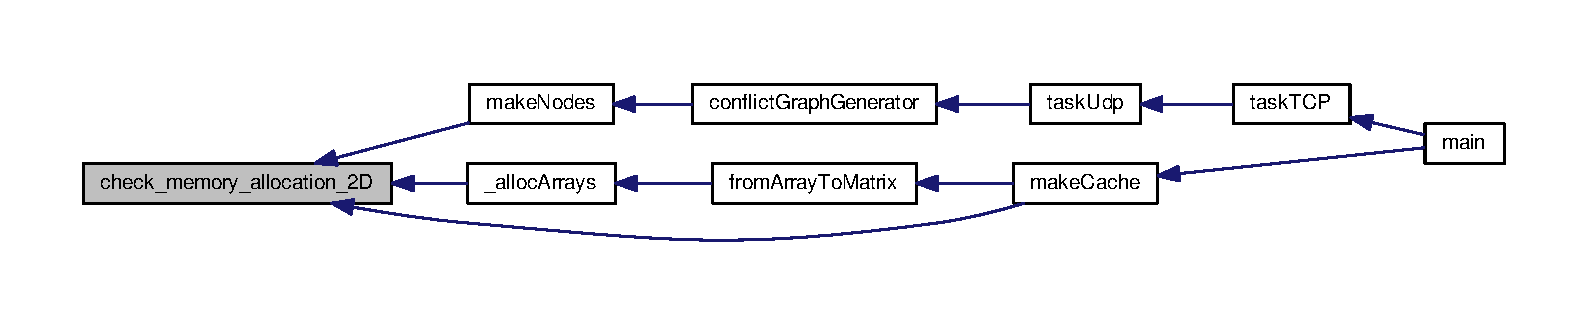
\includegraphics[width=350pt]{CheckFunction_8h_a12a11983f3c936451eabd25a2f89ceec_icgraph}
\end{center}
\end{figure}


\hypertarget{CheckFunction_8h_a917179e80dd117e16637036184490105}{\index{Check\-Function.\-h@{Check\-Function.\-h}!check\-\_\-memory\-\_\-allocation\-\_\-3\-D@{check\-\_\-memory\-\_\-allocation\-\_\-3\-D}}
\index{check\-\_\-memory\-\_\-allocation\-\_\-3\-D@{check\-\_\-memory\-\_\-allocation\-\_\-3\-D}!CheckFunction.h@{Check\-Function.\-h}}
\subsubsection[{check\-\_\-memory\-\_\-allocation\-\_\-3\-D}]{\setlength{\rightskip}{0pt plus 5cm}void check\-\_\-memory\-\_\-allocation\-\_\-3\-D (
\begin{DoxyParamCaption}
\item[{int $\ast$$\ast$$\ast$}]{pt, }
\item[{string}]{msg}
\end{DoxyParamCaption}
)}}\label{CheckFunction_8h_a917179e80dd117e16637036184490105}


Here is the caller graph for this function\-:
\nopagebreak
\begin{figure}[H]
\begin{center}
\leavevmode
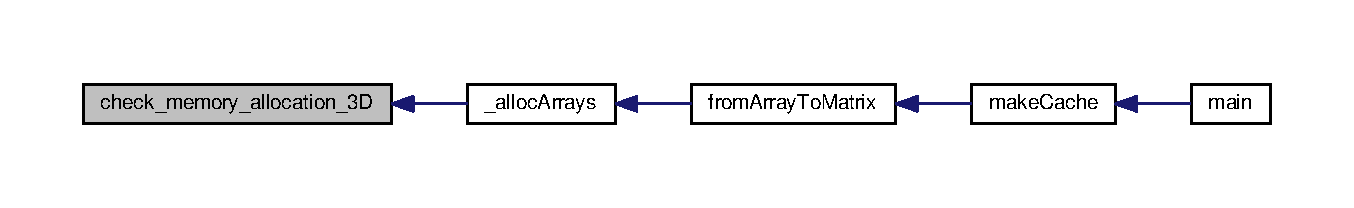
\includegraphics[width=350pt]{CheckFunction_8h_a917179e80dd117e16637036184490105_icgraph}
\end{center}
\end{figure}


\hypertarget{CheckFunction_8h_ad40ce34cc1edd61fbfd997fcf9eaa774}{\index{Check\-Function.\-h@{Check\-Function.\-h}!check\-\_\-memory\-\_\-double\-\_\-allocation\-\_\-1\-D@{check\-\_\-memory\-\_\-double\-\_\-allocation\-\_\-1\-D}}
\index{check\-\_\-memory\-\_\-double\-\_\-allocation\-\_\-1\-D@{check\-\_\-memory\-\_\-double\-\_\-allocation\-\_\-1\-D}!CheckFunction.h@{Check\-Function.\-h}}
\subsubsection[{check\-\_\-memory\-\_\-double\-\_\-allocation\-\_\-1\-D}]{\setlength{\rightskip}{0pt plus 5cm}void check\-\_\-memory\-\_\-double\-\_\-allocation\-\_\-1\-D (
\begin{DoxyParamCaption}
\item[{double $\ast$}]{pt, }
\item[{string}]{msg}
\end{DoxyParamCaption}
)}}\label{CheckFunction_8h_ad40ce34cc1edd61fbfd997fcf9eaa774}


Here is the caller graph for this function\-:
\nopagebreak
\begin{figure}[H]
\begin{center}
\leavevmode
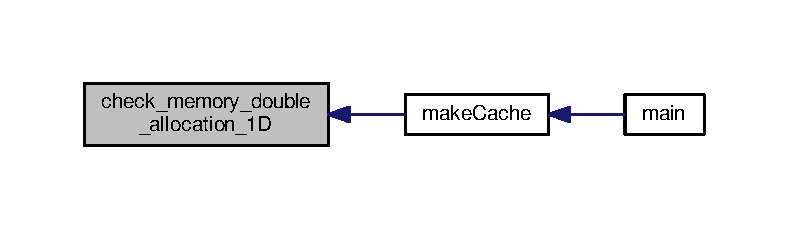
\includegraphics[width=350pt]{CheckFunction_8h_ad40ce34cc1edd61fbfd997fcf9eaa774_icgraph}
\end{center}
\end{figure}


\hypertarget{CheckFunction_8h_a60ac9977b6ad887e42be5d608b7c3384}{\index{Check\-Function.\-h@{Check\-Function.\-h}!check\-\_\-memory\-\_\-double\-\_\-allocation\-\_\-2\-D@{check\-\_\-memory\-\_\-double\-\_\-allocation\-\_\-2\-D}}
\index{check\-\_\-memory\-\_\-double\-\_\-allocation\-\_\-2\-D@{check\-\_\-memory\-\_\-double\-\_\-allocation\-\_\-2\-D}!CheckFunction.h@{Check\-Function.\-h}}
\subsubsection[{check\-\_\-memory\-\_\-double\-\_\-allocation\-\_\-2\-D}]{\setlength{\rightskip}{0pt plus 5cm}void check\-\_\-memory\-\_\-double\-\_\-allocation\-\_\-2\-D (
\begin{DoxyParamCaption}
\item[{double $\ast$$\ast$}]{pt, }
\item[{string}]{msg}
\end{DoxyParamCaption}
)}}\label{CheckFunction_8h_a60ac9977b6ad887e42be5d608b7c3384}


Here is the caller graph for this function\-:
\nopagebreak
\begin{figure}[H]
\begin{center}
\leavevmode
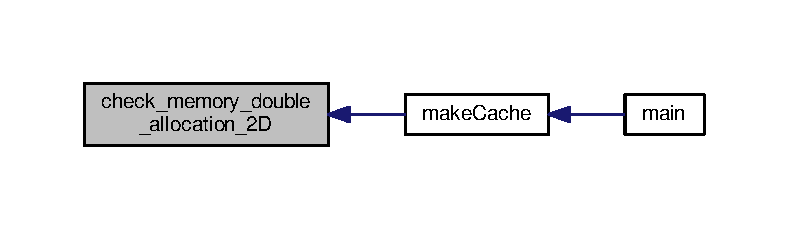
\includegraphics[width=350pt]{CheckFunction_8h_a60ac9977b6ad887e42be5d608b7c3384_icgraph}
\end{center}
\end{figure}



\hypertarget{ConflictGraph_8cpp}{\section{Conflict\-Graph.\-cpp File Reference}
\label{ConflictGraph_8cpp}\index{Conflict\-Graph.\-cpp@{Conflict\-Graph.\-cpp}}
}


File to generate the confict graph to perform the algorithm.  


{\ttfamily \#include \char`\"{}Conflict\-Graph.\-h\char`\"{}}\\*
Include dependency graph for Conflict\-Graph.\-cpp\-:
\nopagebreak
\begin{figure}[H]
\begin{center}
\leavevmode
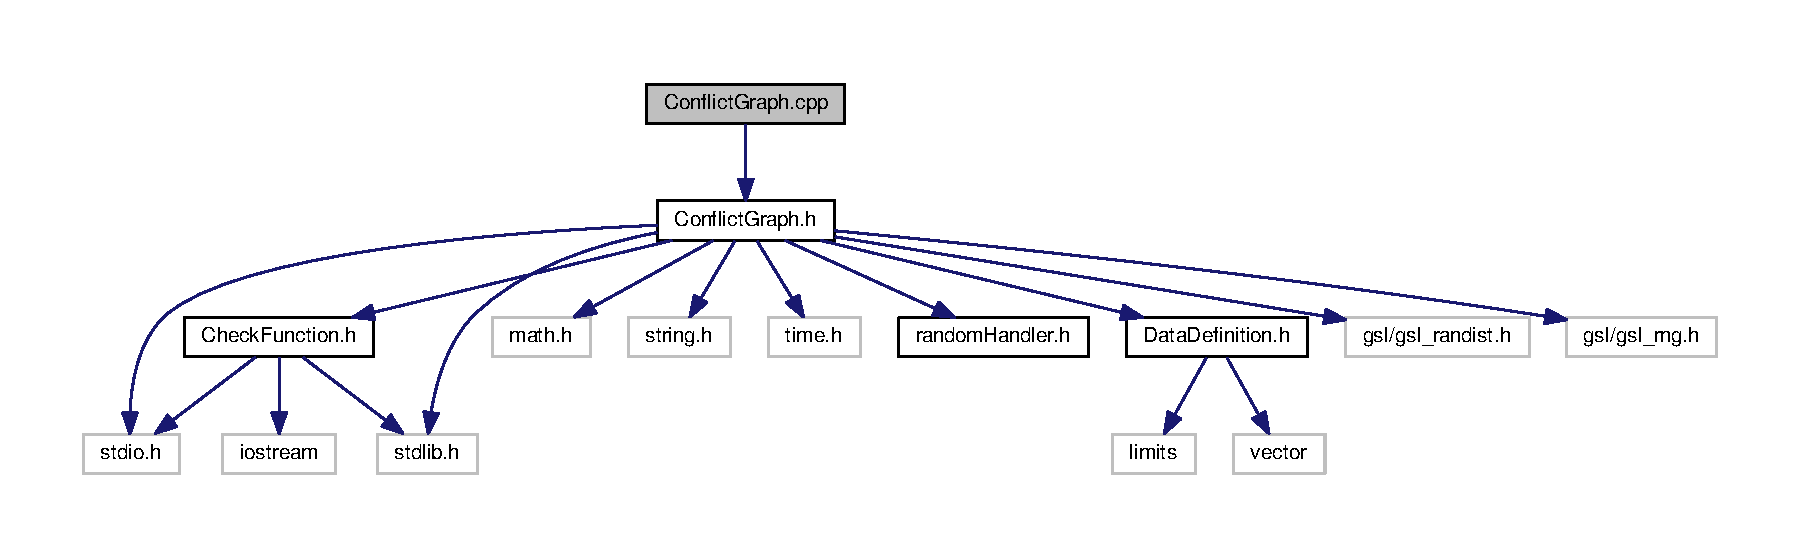
\includegraphics[width=350pt]{ConflictGraph_8cpp__incl}
\end{center}
\end{figure}
\subsection*{Functions}
\begin{DoxyCompactItemize}
\item 
void \hyperlink{ConflictGraph_8cpp_ac3cb25bddc4ccb9b9e9b05d5d6e10f15}{compute\-Number\-Of\-Nodes} ()
\item 
void \hyperlink{ConflictGraph_8cpp_a6de92953bce9d470b645baaa6c546c8c}{make\-Nodes} ()
\item 
void \hyperlink{ConflictGraph_8cpp_abc996d20ffbbc06664b48239600ff7c0}{make\-Edges} ()
\item 
void \hyperlink{ConflictGraph_8cpp_a2d6220650beea54f048db3face9c7b84}{\-\_\-dealloc} ()
\item 
\hyperlink{DataDefinition_8h_a1601a7ee6f4213e7d70430cefa083def}{cf\-\_\-data} \hyperlink{ConflictGraph_8cpp_a1cc64a8f4dc3bd9f1c991abd75432539}{conflict\-Graph\-Generator} (\hyperlink{DataDefinition_8h_aa8ca5572763177379406da03176d0ef9}{data\-\_\-matrix} \hyperlink{server_8cpp_aae9fcbe0ed0ac37c492508691173561d}{data})
\end{DoxyCompactItemize}
\subsection*{Variables}
\begin{DoxyCompactItemize}
\item 
int \hyperlink{ConflictGraph_8cpp_a2f6dbcf4fcf737ed9e4bcfbba6a961fa}{n\-\_\-utenti}
\item 
int \hyperlink{ConflictGraph_8cpp_abd950309ddc65353a014b00c8c4a11b0}{m\-\_\-files}
\item 
int $\ast$ \hyperlink{ConflictGraph_8cpp_a1d12de4f14bfff1b963f424aac823fd5}{b\-\_\-chuncks}
\item 
int \hyperlink{ConflictGraph_8cpp_a17649fbb0d4033d3a77ae6c5831c21f2}{n\-\_\-nodi}
\item 
int \hyperlink{ConflictGraph_8cpp_ab703df34671c9674648d9da3a1d4059a}{m\-\_\-archi}
\item 
int $\ast$$\ast$$\ast$ \hyperlink{ConflictGraph_8cpp_a22d1b39fa2b1c594a8f6d2d29df487c0}{Ind} = N\-U\-L\-L
\item 
int $\ast$ \hyperlink{ConflictGraph_8cpp_a573d3a82580801c056cba08685045cd5}{Q} = N\-U\-L\-L
\item 
int $\ast$$\ast$ \hyperlink{ConflictGraph_8cpp_a8f647323f1ed413f8bf0d8fd6029d475}{Q\-\_\-chuncks} = N\-U\-L\-L
\item 
int $\ast$$\ast$ \hyperlink{ConflictGraph_8cpp_af5bff42832b4870240fe6283fe657582}{Matrix\-\_\-\-Adj} = N\-U\-L\-L
\item 
\hyperlink{DataDefinition_8h_a65ad3efc6589d7d39f5a6813fd74a7d2}{nodo} $\ast$ \hyperlink{ConflictGraph_8cpp_ad37a9f79256fe09ba826524c993d5225}{nodes} = N\-U\-L\-L
\end{DoxyCompactItemize}


\subsection{Detailed Description}
File to generate the confict graph to perform the algorithm. 

\subsection{Function Documentation}
\hypertarget{ConflictGraph_8cpp_a2d6220650beea54f048db3face9c7b84}{\index{Conflict\-Graph.\-cpp@{Conflict\-Graph.\-cpp}!\-\_\-dealloc@{\-\_\-dealloc}}
\index{\-\_\-dealloc@{\-\_\-dealloc}!ConflictGraph.cpp@{Conflict\-Graph.\-cpp}}
\subsubsection[{\-\_\-dealloc}]{\setlength{\rightskip}{0pt plus 5cm}void \-\_\-dealloc (
\begin{DoxyParamCaption}
{}
\end{DoxyParamCaption}
)}}\label{ConflictGraph_8cpp_a2d6220650beea54f048db3face9c7b84}
\hypertarget{ConflictGraph_8cpp_ac3cb25bddc4ccb9b9e9b05d5d6e10f15}{\index{Conflict\-Graph.\-cpp@{Conflict\-Graph.\-cpp}!compute\-Number\-Of\-Nodes@{compute\-Number\-Of\-Nodes}}
\index{compute\-Number\-Of\-Nodes@{compute\-Number\-Of\-Nodes}!ConflictGraph.cpp@{Conflict\-Graph.\-cpp}}
\subsubsection[{compute\-Number\-Of\-Nodes}]{\setlength{\rightskip}{0pt plus 5cm}void compute\-Number\-Of\-Nodes (
\begin{DoxyParamCaption}
{}
\end{DoxyParamCaption}
)}}\label{ConflictGraph_8cpp_ac3cb25bddc4ccb9b9e9b05d5d6e10f15}


Here is the caller graph for this function\-:
\nopagebreak
\begin{figure}[H]
\begin{center}
\leavevmode
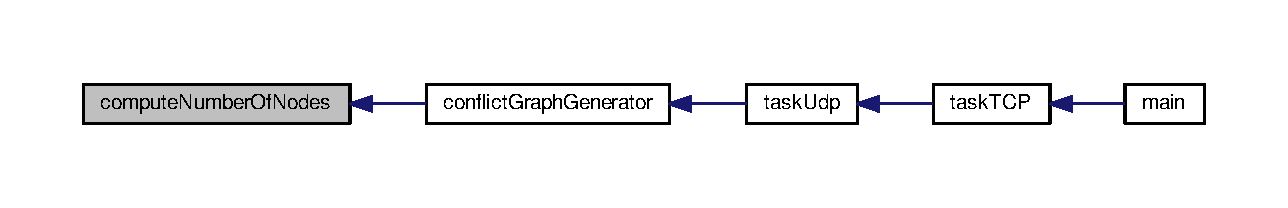
\includegraphics[width=350pt]{ConflictGraph_8cpp_ac3cb25bddc4ccb9b9e9b05d5d6e10f15_icgraph}
\end{center}
\end{figure}


\hypertarget{ConflictGraph_8cpp_a1cc64a8f4dc3bd9f1c991abd75432539}{\index{Conflict\-Graph.\-cpp@{Conflict\-Graph.\-cpp}!conflict\-Graph\-Generator@{conflict\-Graph\-Generator}}
\index{conflict\-Graph\-Generator@{conflict\-Graph\-Generator}!ConflictGraph.cpp@{Conflict\-Graph.\-cpp}}
\subsubsection[{conflict\-Graph\-Generator}]{\setlength{\rightskip}{0pt plus 5cm}{\bf cf\-\_\-data} conflict\-Graph\-Generator (
\begin{DoxyParamCaption}
\item[{{\bf data\-\_\-matrix}}]{data}
\end{DoxyParamCaption}
)}}\label{ConflictGraph_8cpp_a1cc64a8f4dc3bd9f1c991abd75432539}


Here is the call graph for this function\-:
\nopagebreak
\begin{figure}[H]
\begin{center}
\leavevmode
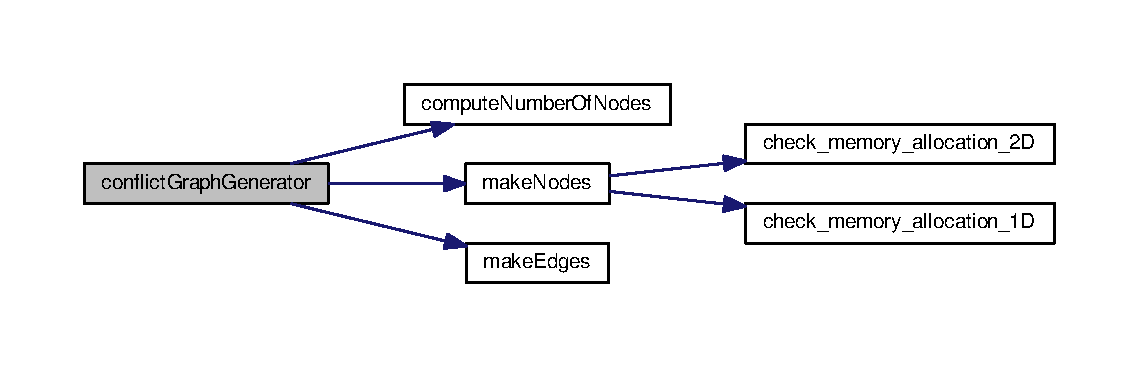
\includegraphics[width=350pt]{ConflictGraph_8cpp_a1cc64a8f4dc3bd9f1c991abd75432539_cgraph}
\end{center}
\end{figure}




Here is the caller graph for this function\-:
\nopagebreak
\begin{figure}[H]
\begin{center}
\leavevmode
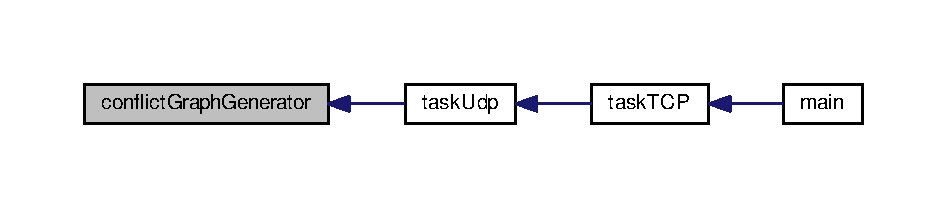
\includegraphics[width=350pt]{ConflictGraph_8cpp_a1cc64a8f4dc3bd9f1c991abd75432539_icgraph}
\end{center}
\end{figure}


\hypertarget{ConflictGraph_8cpp_abc996d20ffbbc06664b48239600ff7c0}{\index{Conflict\-Graph.\-cpp@{Conflict\-Graph.\-cpp}!make\-Edges@{make\-Edges}}
\index{make\-Edges@{make\-Edges}!ConflictGraph.cpp@{Conflict\-Graph.\-cpp}}
\subsubsection[{make\-Edges}]{\setlength{\rightskip}{0pt plus 5cm}void make\-Edges (
\begin{DoxyParamCaption}
{}
\end{DoxyParamCaption}
)}}\label{ConflictGraph_8cpp_abc996d20ffbbc06664b48239600ff7c0}


Here is the caller graph for this function\-:
\nopagebreak
\begin{figure}[H]
\begin{center}
\leavevmode
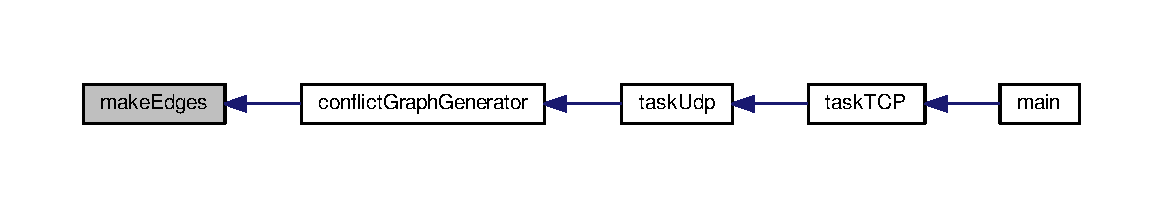
\includegraphics[width=350pt]{ConflictGraph_8cpp_abc996d20ffbbc06664b48239600ff7c0_icgraph}
\end{center}
\end{figure}


\hypertarget{ConflictGraph_8cpp_a6de92953bce9d470b645baaa6c546c8c}{\index{Conflict\-Graph.\-cpp@{Conflict\-Graph.\-cpp}!make\-Nodes@{make\-Nodes}}
\index{make\-Nodes@{make\-Nodes}!ConflictGraph.cpp@{Conflict\-Graph.\-cpp}}
\subsubsection[{make\-Nodes}]{\setlength{\rightskip}{0pt plus 5cm}void make\-Nodes (
\begin{DoxyParamCaption}
{}
\end{DoxyParamCaption}
)}}\label{ConflictGraph_8cpp_a6de92953bce9d470b645baaa6c546c8c}


Here is the call graph for this function\-:
\nopagebreak
\begin{figure}[H]
\begin{center}
\leavevmode
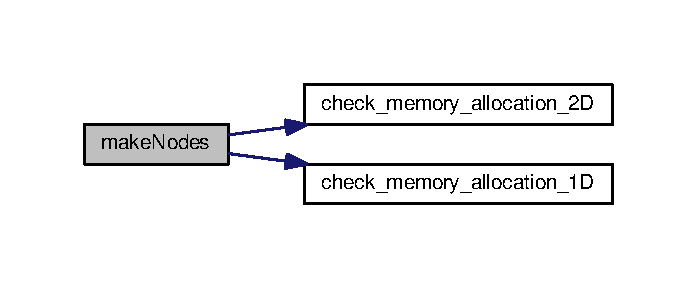
\includegraphics[width=334pt]{ConflictGraph_8cpp_a6de92953bce9d470b645baaa6c546c8c_cgraph}
\end{center}
\end{figure}




Here is the caller graph for this function\-:
\nopagebreak
\begin{figure}[H]
\begin{center}
\leavevmode
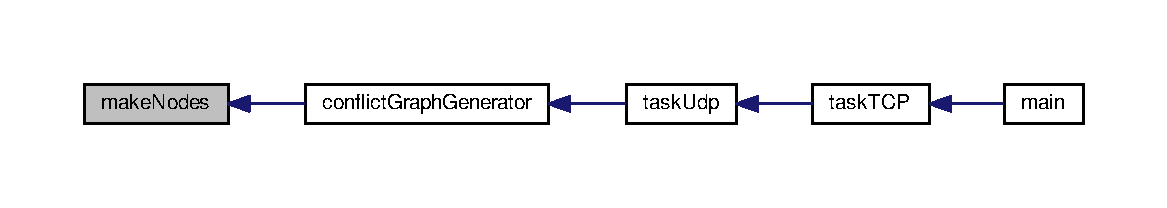
\includegraphics[width=350pt]{ConflictGraph_8cpp_a6de92953bce9d470b645baaa6c546c8c_icgraph}
\end{center}
\end{figure}




\subsection{Variable Documentation}
\hypertarget{ConflictGraph_8cpp_a1d12de4f14bfff1b963f424aac823fd5}{\index{Conflict\-Graph.\-cpp@{Conflict\-Graph.\-cpp}!b\-\_\-chuncks@{b\-\_\-chuncks}}
\index{b\-\_\-chuncks@{b\-\_\-chuncks}!ConflictGraph.cpp@{Conflict\-Graph.\-cpp}}
\subsubsection[{b\-\_\-chuncks}]{\setlength{\rightskip}{0pt plus 5cm}int$\ast$ b\-\_\-chuncks}}\label{ConflictGraph_8cpp_a1d12de4f14bfff1b963f424aac823fd5}
\hypertarget{ConflictGraph_8cpp_a22d1b39fa2b1c594a8f6d2d29df487c0}{\index{Conflict\-Graph.\-cpp@{Conflict\-Graph.\-cpp}!Ind@{Ind}}
\index{Ind@{Ind}!ConflictGraph.cpp@{Conflict\-Graph.\-cpp}}
\subsubsection[{Ind}]{\setlength{\rightskip}{0pt plus 5cm}int$\ast$$\ast$$\ast$ Ind = N\-U\-L\-L}}\label{ConflictGraph_8cpp_a22d1b39fa2b1c594a8f6d2d29df487c0}
\hypertarget{ConflictGraph_8cpp_ab703df34671c9674648d9da3a1d4059a}{\index{Conflict\-Graph.\-cpp@{Conflict\-Graph.\-cpp}!m\-\_\-archi@{m\-\_\-archi}}
\index{m\-\_\-archi@{m\-\_\-archi}!ConflictGraph.cpp@{Conflict\-Graph.\-cpp}}
\subsubsection[{m\-\_\-archi}]{\setlength{\rightskip}{0pt plus 5cm}int m\-\_\-archi}}\label{ConflictGraph_8cpp_ab703df34671c9674648d9da3a1d4059a}
\hypertarget{ConflictGraph_8cpp_abd950309ddc65353a014b00c8c4a11b0}{\index{Conflict\-Graph.\-cpp@{Conflict\-Graph.\-cpp}!m\-\_\-files@{m\-\_\-files}}
\index{m\-\_\-files@{m\-\_\-files}!ConflictGraph.cpp@{Conflict\-Graph.\-cpp}}
\subsubsection[{m\-\_\-files}]{\setlength{\rightskip}{0pt plus 5cm}int m\-\_\-files}}\label{ConflictGraph_8cpp_abd950309ddc65353a014b00c8c4a11b0}
\hypertarget{ConflictGraph_8cpp_af5bff42832b4870240fe6283fe657582}{\index{Conflict\-Graph.\-cpp@{Conflict\-Graph.\-cpp}!Matrix\-\_\-\-Adj@{Matrix\-\_\-\-Adj}}
\index{Matrix\-\_\-\-Adj@{Matrix\-\_\-\-Adj}!ConflictGraph.cpp@{Conflict\-Graph.\-cpp}}
\subsubsection[{Matrix\-\_\-\-Adj}]{\setlength{\rightskip}{0pt plus 5cm}int$\ast$$\ast$ Matrix\-\_\-\-Adj = N\-U\-L\-L}}\label{ConflictGraph_8cpp_af5bff42832b4870240fe6283fe657582}
\hypertarget{ConflictGraph_8cpp_a17649fbb0d4033d3a77ae6c5831c21f2}{\index{Conflict\-Graph.\-cpp@{Conflict\-Graph.\-cpp}!n\-\_\-nodi@{n\-\_\-nodi}}
\index{n\-\_\-nodi@{n\-\_\-nodi}!ConflictGraph.cpp@{Conflict\-Graph.\-cpp}}
\subsubsection[{n\-\_\-nodi}]{\setlength{\rightskip}{0pt plus 5cm}int n\-\_\-nodi}}\label{ConflictGraph_8cpp_a17649fbb0d4033d3a77ae6c5831c21f2}
\hypertarget{ConflictGraph_8cpp_a2f6dbcf4fcf737ed9e4bcfbba6a961fa}{\index{Conflict\-Graph.\-cpp@{Conflict\-Graph.\-cpp}!n\-\_\-utenti@{n\-\_\-utenti}}
\index{n\-\_\-utenti@{n\-\_\-utenti}!ConflictGraph.cpp@{Conflict\-Graph.\-cpp}}
\subsubsection[{n\-\_\-utenti}]{\setlength{\rightskip}{0pt plus 5cm}int n\-\_\-utenti}}\label{ConflictGraph_8cpp_a2f6dbcf4fcf737ed9e4bcfbba6a961fa}
\hypertarget{ConflictGraph_8cpp_ad37a9f79256fe09ba826524c993d5225}{\index{Conflict\-Graph.\-cpp@{Conflict\-Graph.\-cpp}!nodes@{nodes}}
\index{nodes@{nodes}!ConflictGraph.cpp@{Conflict\-Graph.\-cpp}}
\subsubsection[{nodes}]{\setlength{\rightskip}{0pt plus 5cm}{\bf nodo}$\ast$ nodes = N\-U\-L\-L}}\label{ConflictGraph_8cpp_ad37a9f79256fe09ba826524c993d5225}
\hypertarget{ConflictGraph_8cpp_a573d3a82580801c056cba08685045cd5}{\index{Conflict\-Graph.\-cpp@{Conflict\-Graph.\-cpp}!Q@{Q}}
\index{Q@{Q}!ConflictGraph.cpp@{Conflict\-Graph.\-cpp}}
\subsubsection[{Q}]{\setlength{\rightskip}{0pt plus 5cm}int$\ast$ Q = N\-U\-L\-L}}\label{ConflictGraph_8cpp_a573d3a82580801c056cba08685045cd5}
\hypertarget{ConflictGraph_8cpp_a8f647323f1ed413f8bf0d8fd6029d475}{\index{Conflict\-Graph.\-cpp@{Conflict\-Graph.\-cpp}!Q\-\_\-chuncks@{Q\-\_\-chuncks}}
\index{Q\-\_\-chuncks@{Q\-\_\-chuncks}!ConflictGraph.cpp@{Conflict\-Graph.\-cpp}}
\subsubsection[{Q\-\_\-chuncks}]{\setlength{\rightskip}{0pt plus 5cm}int$\ast$$\ast$ Q\-\_\-chuncks = N\-U\-L\-L}}\label{ConflictGraph_8cpp_a8f647323f1ed413f8bf0d8fd6029d475}

\hypertarget{ConflictGraph_8h}{\section{Conflict\-Graph.\-h File Reference}
\label{ConflictGraph_8h}\index{Conflict\-Graph.\-h@{Conflict\-Graph.\-h}}
}
{\ttfamily \#include $<$stdio.\-h$>$}\\*
{\ttfamily \#include $<$stdlib.\-h$>$}\\*
{\ttfamily \#include $<$math.\-h$>$}\\*
{\ttfamily \#include $<$string.\-h$>$}\\*
{\ttfamily \#include $<$time.\-h$>$}\\*
{\ttfamily \#include \char`\"{}random\-Handler.\-h\char`\"{}}\\*
{\ttfamily \#include \char`\"{}Check\-Function.\-h\char`\"{}}\\*
{\ttfamily \#include \char`\"{}Data\-Definition.\-h\char`\"{}}\\*
{\ttfamily \#include $<$gsl/gsl\-\_\-randist.\-h$>$}\\*
{\ttfamily \#include $<$gsl/gsl\-\_\-rng.\-h$>$}\\*
Include dependency graph for Conflict\-Graph.\-h\-:
\nopagebreak
\begin{figure}[H]
\begin{center}
\leavevmode
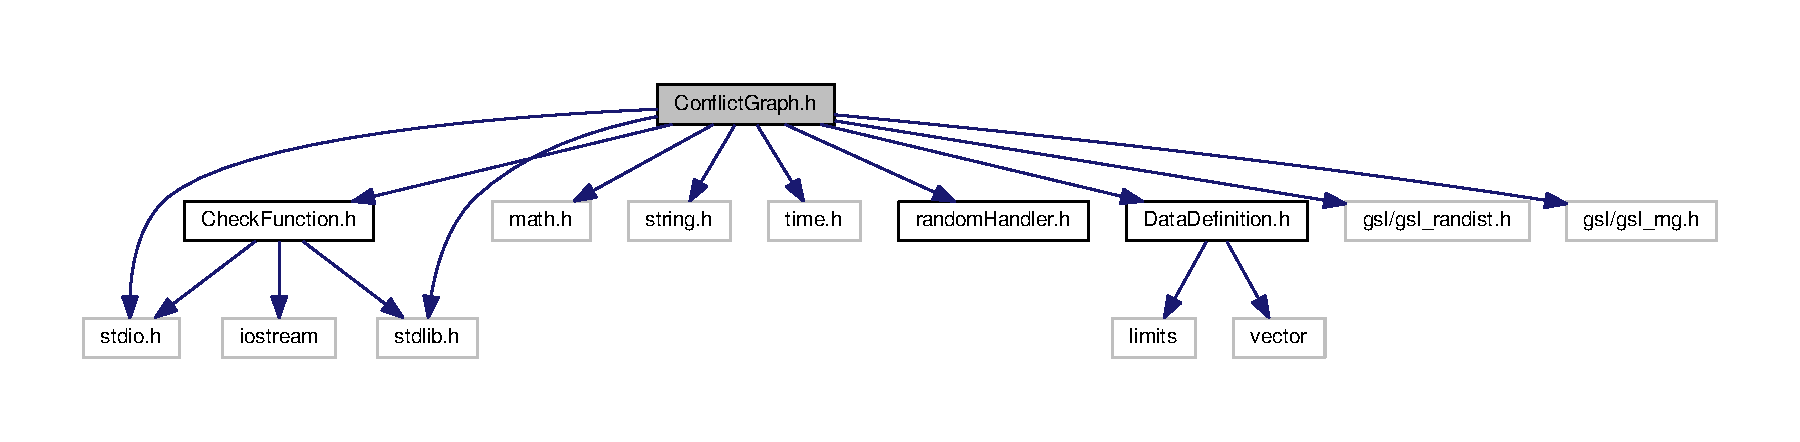
\includegraphics[width=350pt]{ConflictGraph_8h__incl}
\end{center}
\end{figure}
This graph shows which files directly or indirectly include this file\-:
\nopagebreak
\begin{figure}[H]
\begin{center}
\leavevmode
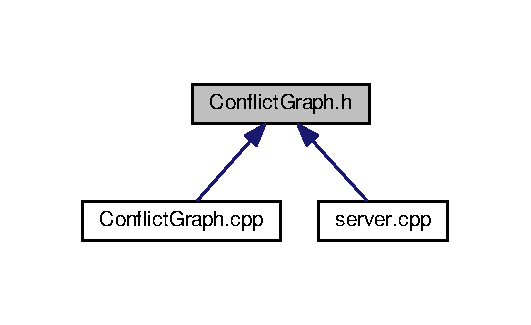
\includegraphics[width=255pt]{ConflictGraph_8h__dep__incl}
\end{center}
\end{figure}
\subsection*{Functions}
\begin{DoxyCompactItemize}
\item 
void \hyperlink{ConflictGraph_8h_a2d6220650beea54f048db3face9c7b84}{\-\_\-dealloc} ()
\item 
void \hyperlink{ConflictGraph_8h_ac3cb25bddc4ccb9b9e9b05d5d6e10f15}{compute\-Number\-Of\-Nodes} ()
\item 
void \hyperlink{ConflictGraph_8h_a6de92953bce9d470b645baaa6c546c8c}{make\-Nodes} ()
\item 
void \hyperlink{ConflictGraph_8h_abc996d20ffbbc06664b48239600ff7c0}{make\-Edges} ()
\item 
\hyperlink{DataDefinition_8h_a1601a7ee6f4213e7d70430cefa083def}{cf\-\_\-data} \hyperlink{ConflictGraph_8h_a1cc64a8f4dc3bd9f1c991abd75432539}{conflict\-Graph\-Generator} (\hyperlink{DataDefinition_8h_aa8ca5572763177379406da03176d0ef9}{data\-\_\-matrix} \hyperlink{server_8cpp_aae9fcbe0ed0ac37c492508691173561d}{data})
\end{DoxyCompactItemize}


\subsection{Function Documentation}
\hypertarget{ConflictGraph_8h_a2d6220650beea54f048db3face9c7b84}{\index{Conflict\-Graph.\-h@{Conflict\-Graph.\-h}!\-\_\-dealloc@{\-\_\-dealloc}}
\index{\-\_\-dealloc@{\-\_\-dealloc}!ConflictGraph.h@{Conflict\-Graph.\-h}}
\subsubsection[{\-\_\-dealloc}]{\setlength{\rightskip}{0pt plus 5cm}void \-\_\-dealloc (
\begin{DoxyParamCaption}
{}
\end{DoxyParamCaption}
)}}\label{ConflictGraph_8h_a2d6220650beea54f048db3face9c7b84}
\hypertarget{ConflictGraph_8h_ac3cb25bddc4ccb9b9e9b05d5d6e10f15}{\index{Conflict\-Graph.\-h@{Conflict\-Graph.\-h}!compute\-Number\-Of\-Nodes@{compute\-Number\-Of\-Nodes}}
\index{compute\-Number\-Of\-Nodes@{compute\-Number\-Of\-Nodes}!ConflictGraph.h@{Conflict\-Graph.\-h}}
\subsubsection[{compute\-Number\-Of\-Nodes}]{\setlength{\rightskip}{0pt plus 5cm}void compute\-Number\-Of\-Nodes (
\begin{DoxyParamCaption}
{}
\end{DoxyParamCaption}
)}}\label{ConflictGraph_8h_ac3cb25bddc4ccb9b9e9b05d5d6e10f15}


Here is the caller graph for this function\-:
\nopagebreak
\begin{figure}[H]
\begin{center}
\leavevmode
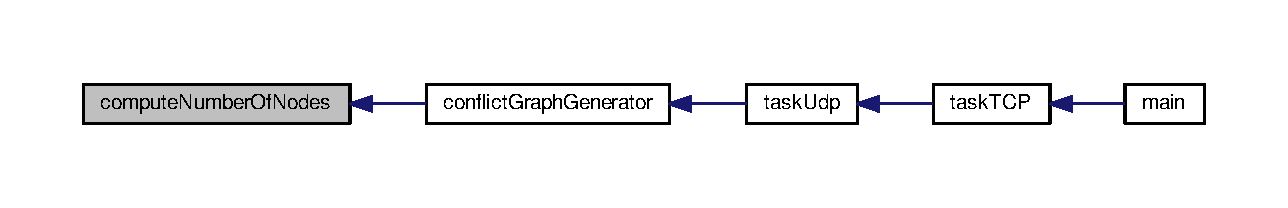
\includegraphics[width=350pt]{ConflictGraph_8h_ac3cb25bddc4ccb9b9e9b05d5d6e10f15_icgraph}
\end{center}
\end{figure}


\hypertarget{ConflictGraph_8h_a1cc64a8f4dc3bd9f1c991abd75432539}{\index{Conflict\-Graph.\-h@{Conflict\-Graph.\-h}!conflict\-Graph\-Generator@{conflict\-Graph\-Generator}}
\index{conflict\-Graph\-Generator@{conflict\-Graph\-Generator}!ConflictGraph.h@{Conflict\-Graph.\-h}}
\subsubsection[{conflict\-Graph\-Generator}]{\setlength{\rightskip}{0pt plus 5cm}{\bf cf\-\_\-data} conflict\-Graph\-Generator (
\begin{DoxyParamCaption}
\item[{{\bf data\-\_\-matrix}}]{data}
\end{DoxyParamCaption}
)}}\label{ConflictGraph_8h_a1cc64a8f4dc3bd9f1c991abd75432539}


Here is the call graph for this function\-:
\nopagebreak
\begin{figure}[H]
\begin{center}
\leavevmode
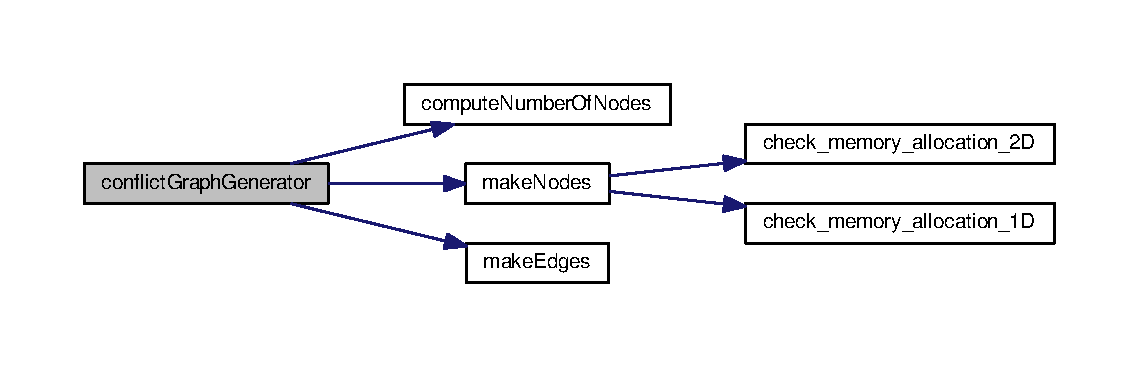
\includegraphics[width=350pt]{ConflictGraph_8h_a1cc64a8f4dc3bd9f1c991abd75432539_cgraph}
\end{center}
\end{figure}




Here is the caller graph for this function\-:
\nopagebreak
\begin{figure}[H]
\begin{center}
\leavevmode
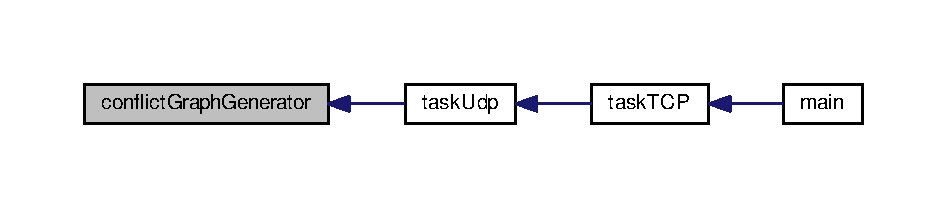
\includegraphics[width=350pt]{ConflictGraph_8h_a1cc64a8f4dc3bd9f1c991abd75432539_icgraph}
\end{center}
\end{figure}


\hypertarget{ConflictGraph_8h_abc996d20ffbbc06664b48239600ff7c0}{\index{Conflict\-Graph.\-h@{Conflict\-Graph.\-h}!make\-Edges@{make\-Edges}}
\index{make\-Edges@{make\-Edges}!ConflictGraph.h@{Conflict\-Graph.\-h}}
\subsubsection[{make\-Edges}]{\setlength{\rightskip}{0pt plus 5cm}void make\-Edges (
\begin{DoxyParamCaption}
{}
\end{DoxyParamCaption}
)}}\label{ConflictGraph_8h_abc996d20ffbbc06664b48239600ff7c0}


Here is the caller graph for this function\-:
\nopagebreak
\begin{figure}[H]
\begin{center}
\leavevmode
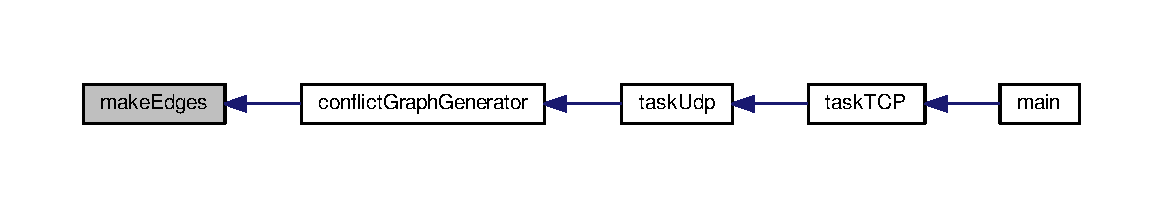
\includegraphics[width=350pt]{ConflictGraph_8h_abc996d20ffbbc06664b48239600ff7c0_icgraph}
\end{center}
\end{figure}


\hypertarget{ConflictGraph_8h_a6de92953bce9d470b645baaa6c546c8c}{\index{Conflict\-Graph.\-h@{Conflict\-Graph.\-h}!make\-Nodes@{make\-Nodes}}
\index{make\-Nodes@{make\-Nodes}!ConflictGraph.h@{Conflict\-Graph.\-h}}
\subsubsection[{make\-Nodes}]{\setlength{\rightskip}{0pt plus 5cm}void make\-Nodes (
\begin{DoxyParamCaption}
{}
\end{DoxyParamCaption}
)}}\label{ConflictGraph_8h_a6de92953bce9d470b645baaa6c546c8c}


Here is the call graph for this function\-:
\nopagebreak
\begin{figure}[H]
\begin{center}
\leavevmode
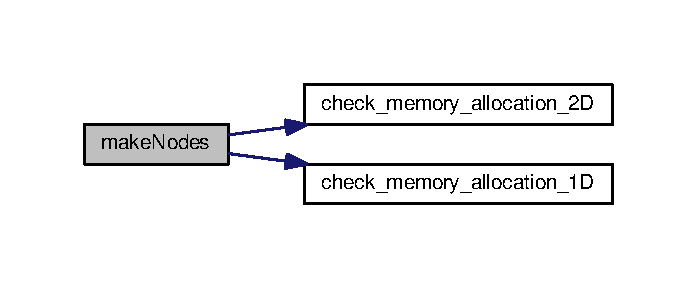
\includegraphics[width=334pt]{ConflictGraph_8h_a6de92953bce9d470b645baaa6c546c8c_cgraph}
\end{center}
\end{figure}




Here is the caller graph for this function\-:
\nopagebreak
\begin{figure}[H]
\begin{center}
\leavevmode
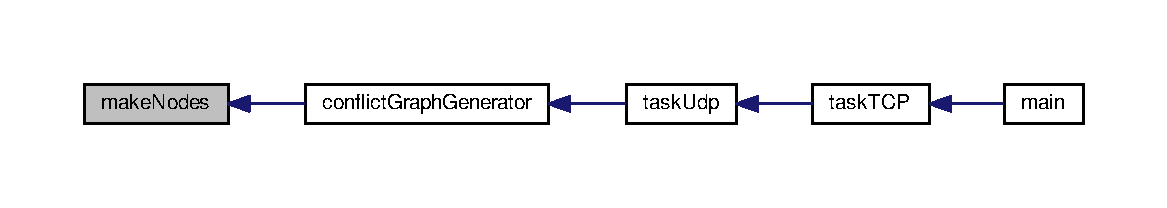
\includegraphics[width=350pt]{ConflictGraph_8h_a6de92953bce9d470b645baaa6c546c8c_icgraph}
\end{center}
\end{figure}



\hypertarget{DataDefinition_8h}{\section{Data\-Definition.\-h File Reference}
\label{DataDefinition_8h}\index{Data\-Definition.\-h@{Data\-Definition.\-h}}
}
{\ttfamily \#include $<$limits$>$}\\*
{\ttfamily \#include $<$vector$>$}\\*
Include dependency graph for Data\-Definition.\-h\-:
\nopagebreak
\begin{figure}[H]
\begin{center}
\leavevmode
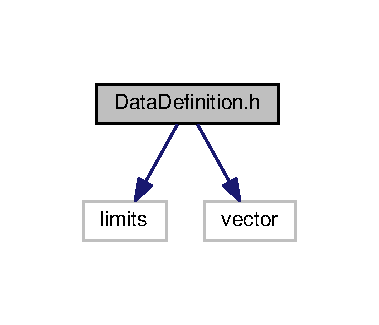
\includegraphics[width=182pt]{DataDefinition_8h__incl}
\end{center}
\end{figure}
This graph shows which files directly or indirectly include this file\-:
\nopagebreak
\begin{figure}[H]
\begin{center}
\leavevmode
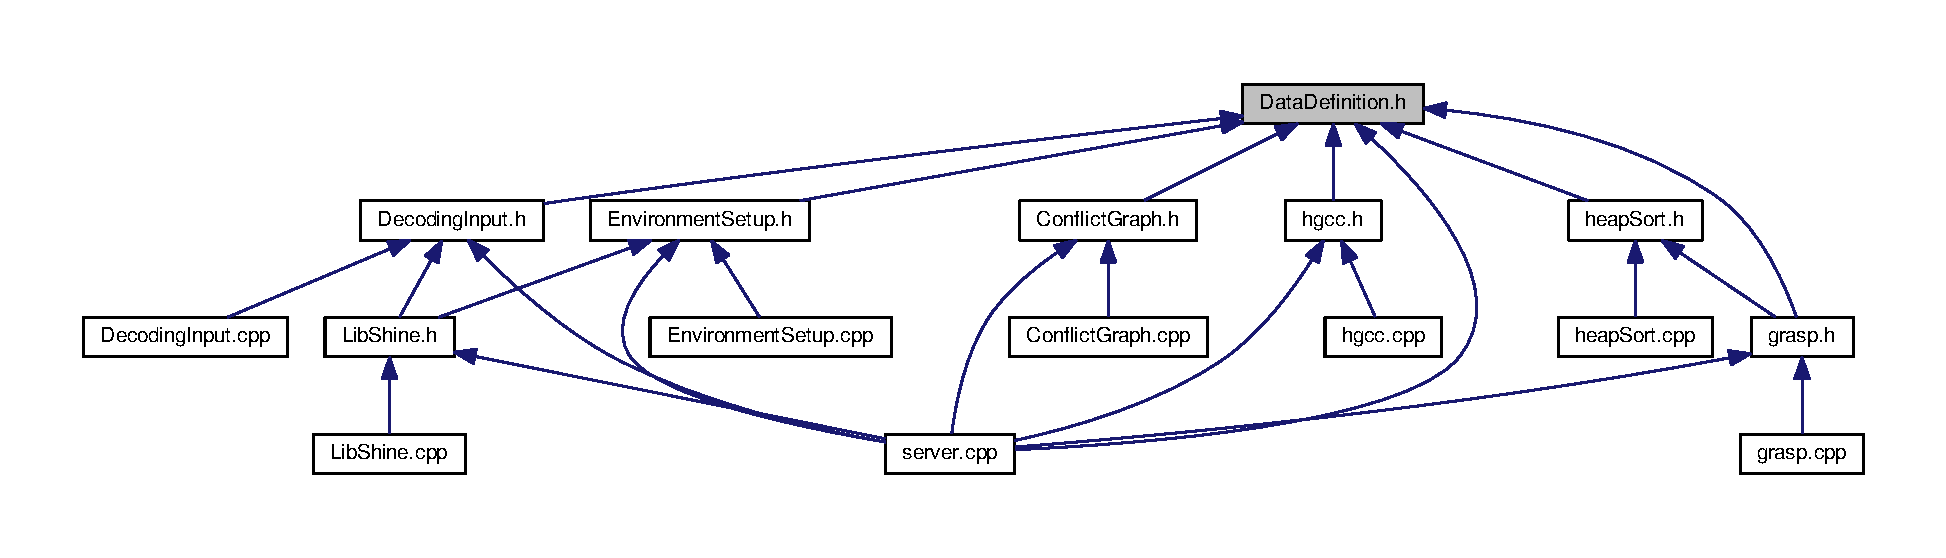
\includegraphics[width=350pt]{DataDefinition_8h__dep__incl}
\end{center}
\end{figure}
\subsection*{Classes}
\begin{DoxyCompactItemize}
\item 
struct \hyperlink{structNODE__LIST__STRUCT}{N\-O\-D\-E\-\_\-\-L\-I\-S\-T\-\_\-\-S\-T\-R\-U\-C\-T}
\item 
struct \hyperlink{structLIST__STRUCT}{L\-I\-S\-T\-\_\-\-S\-T\-R\-U\-C\-T}
\item 
struct \hyperlink{structNODE__SUBSET__STRUCT}{N\-O\-D\-E\-\_\-\-S\-U\-B\-S\-E\-T\-\_\-\-S\-T\-R\-U\-C\-T}
\item 
struct \hyperlink{structSUBSET__STRUCT}{S\-U\-B\-S\-E\-T\-\_\-\-S\-T\-R\-U\-C\-T}
\item 
struct \hyperlink{structNODO}{N\-O\-D\-O}
\item 
struct \hyperlink{structARC__STRUCT}{A\-R\-C\-\_\-\-S\-T\-R\-U\-C\-T}
\item 
struct \hyperlink{structNODE__STRUCT}{N\-O\-D\-E\-\_\-\-S\-T\-R\-U\-C\-T}
\item 
struct \hyperlink{structRCL__LIST__STRUCT}{R\-C\-L\-\_\-\-L\-I\-S\-T\-\_\-\-S\-T\-R\-U\-C\-T}
\item 
struct \hyperlink{structRANDOM__LIST}{R\-A\-N\-D\-O\-M\-\_\-\-L\-I\-S\-T}
\item 
struct \hyperlink{structDATA__MATRIX}{D\-A\-T\-A\-\_\-\-M\-A\-T\-R\-I\-X}
\item 
struct \hyperlink{structCF__DATA}{C\-F\-\_\-\-D\-A\-T\-A}
\item 
struct \hyperlink{structHEADER__TRANSMISSION}{H\-E\-A\-D\-E\-R\-\_\-\-T\-R\-A\-N\-S\-M\-I\-S\-S\-I\-O\-N}
\end{DoxyCompactItemize}
\subsection*{Typedefs}
\begin{DoxyCompactItemize}
\item 
typedef struct \hyperlink{structNODE__LIST__STRUCT}{N\-O\-D\-E\-\_\-\-L\-I\-S\-T\-\_\-\-S\-T\-R\-U\-C\-T} \hyperlink{DataDefinition_8h_a8804182fdd4652d904801ac03e3d9307}{N\-O\-D\-E\-\_\-\-L\-I\-S\-T}
\item 
typedef struct \hyperlink{structLIST__STRUCT}{L\-I\-S\-T\-\_\-\-S\-T\-R\-U\-C\-T} \hyperlink{DataDefinition_8h_a143b53448976e9b1832cf6ae6694a701}{L\-I\-S\-T}
\item 
typedef struct \hyperlink{structNODE__SUBSET__STRUCT}{N\-O\-D\-E\-\_\-\-S\-U\-B\-S\-E\-T\-\_\-\-S\-T\-R\-U\-C\-T} \hyperlink{DataDefinition_8h_a6c7c55bb5cf24ee7e388f70b7564be38}{N\-O\-D\-E\-\_\-\-S\-U\-B\-S\-E\-T}
\item 
typedef struct \hyperlink{structSUBSET__STRUCT}{S\-U\-B\-S\-E\-T\-\_\-\-S\-T\-R\-U\-C\-T} \hyperlink{DataDefinition_8h_a38c2e6950c1677f28fba2435bd224bb9}{S\-U\-B\-S\-E\-T}
\item 
typedef struct \hyperlink{structNODO}{N\-O\-D\-O} \hyperlink{DataDefinition_8h_a65ad3efc6589d7d39f5a6813fd74a7d2}{nodo}
\item 
typedef struct \hyperlink{structARC__STRUCT}{A\-R\-C\-\_\-\-S\-T\-R\-U\-C\-T} \hyperlink{DataDefinition_8h_add2099c08e012faaa979c9b373eda54a}{A\-R\-C}
\item 
typedef struct \hyperlink{structNODE__STRUCT}{N\-O\-D\-E\-\_\-\-S\-T\-R\-U\-C\-T} \hyperlink{DataDefinition_8h_a17b26c913a8eb52ca9efdc06681981b7}{N\-O\-D\-E}
\item 
typedef struct \hyperlink{structRCL__LIST__STRUCT}{R\-C\-L\-\_\-\-L\-I\-S\-T\-\_\-\-S\-T\-R\-U\-C\-T} \hyperlink{DataDefinition_8h_a8c4793b470f20960e0647bcb528a171b}{R\-C\-L\-\_\-\-L\-I\-S\-T}
\item 
typedef struct \hyperlink{structRANDOM__LIST}{R\-A\-N\-D\-O\-M\-\_\-\-L\-I\-S\-T} \hyperlink{DataDefinition_8h_ab991f8d47d6576d7b48a4c8664014e78}{random\-\_\-list}
\item 
typedef struct \hyperlink{structDATA__MATRIX}{D\-A\-T\-A\-\_\-\-M\-A\-T\-R\-I\-X} \hyperlink{DataDefinition_8h_aa8ca5572763177379406da03176d0ef9}{data\-\_\-matrix}
\item 
typedef struct \hyperlink{structCF__DATA}{C\-F\-\_\-\-D\-A\-T\-A} \hyperlink{DataDefinition_8h_a1601a7ee6f4213e7d70430cefa083def}{cf\-\_\-data}
\item 
typedef struct \hyperlink{structHEADER__TRANSMISSION}{H\-E\-A\-D\-E\-R\-\_\-\-T\-R\-A\-N\-S\-M\-I\-S\-S\-I\-O\-N} \hyperlink{DataDefinition_8h_a322105278c15798a807c79187b83e7f7}{header\-\_\-transmission}
\end{DoxyCompactItemize}
\subsection*{Variables}
\begin{DoxyCompactItemize}
\item 
const int \hyperlink{DataDefinition_8h_a14c9dbab105f1b8b8182a022d73e610c}{I\-N\-F} = numeric\-\_\-limits$<$int$>$\-::max()
\end{DoxyCompactItemize}


\subsection{Typedef Documentation}
\hypertarget{DataDefinition_8h_add2099c08e012faaa979c9b373eda54a}{\index{Data\-Definition.\-h@{Data\-Definition.\-h}!A\-R\-C@{A\-R\-C}}
\index{A\-R\-C@{A\-R\-C}!DataDefinition.h@{Data\-Definition.\-h}}
\subsubsection[{A\-R\-C}]{\setlength{\rightskip}{0pt plus 5cm}typedef struct {\bf A\-R\-C\-\_\-\-S\-T\-R\-U\-C\-T} {\bf A\-R\-C}}}\label{DataDefinition_8h_add2099c08e012faaa979c9b373eda54a}
\hypertarget{DataDefinition_8h_a1601a7ee6f4213e7d70430cefa083def}{\index{Data\-Definition.\-h@{Data\-Definition.\-h}!cf\-\_\-data@{cf\-\_\-data}}
\index{cf\-\_\-data@{cf\-\_\-data}!DataDefinition.h@{Data\-Definition.\-h}}
\subsubsection[{cf\-\_\-data}]{\setlength{\rightskip}{0pt plus 5cm}typedef struct {\bf C\-F\-\_\-\-D\-A\-T\-A} {\bf cf\-\_\-data}}}\label{DataDefinition_8h_a1601a7ee6f4213e7d70430cefa083def}
\hypertarget{DataDefinition_8h_aa8ca5572763177379406da03176d0ef9}{\index{Data\-Definition.\-h@{Data\-Definition.\-h}!data\-\_\-matrix@{data\-\_\-matrix}}
\index{data\-\_\-matrix@{data\-\_\-matrix}!DataDefinition.h@{Data\-Definition.\-h}}
\subsubsection[{data\-\_\-matrix}]{\setlength{\rightskip}{0pt plus 5cm}typedef struct {\bf D\-A\-T\-A\-\_\-\-M\-A\-T\-R\-I\-X} {\bf data\-\_\-matrix}}}\label{DataDefinition_8h_aa8ca5572763177379406da03176d0ef9}
\hypertarget{DataDefinition_8h_a322105278c15798a807c79187b83e7f7}{\index{Data\-Definition.\-h@{Data\-Definition.\-h}!header\-\_\-transmission@{header\-\_\-transmission}}
\index{header\-\_\-transmission@{header\-\_\-transmission}!DataDefinition.h@{Data\-Definition.\-h}}
\subsubsection[{header\-\_\-transmission}]{\setlength{\rightskip}{0pt plus 5cm}typedef struct {\bf H\-E\-A\-D\-E\-R\-\_\-\-T\-R\-A\-N\-S\-M\-I\-S\-S\-I\-O\-N} {\bf header\-\_\-transmission}}}\label{DataDefinition_8h_a322105278c15798a807c79187b83e7f7}
\hypertarget{DataDefinition_8h_a143b53448976e9b1832cf6ae6694a701}{\index{Data\-Definition.\-h@{Data\-Definition.\-h}!L\-I\-S\-T@{L\-I\-S\-T}}
\index{L\-I\-S\-T@{L\-I\-S\-T}!DataDefinition.h@{Data\-Definition.\-h}}
\subsubsection[{L\-I\-S\-T}]{\setlength{\rightskip}{0pt plus 5cm}typedef struct {\bf L\-I\-S\-T\-\_\-\-S\-T\-R\-U\-C\-T} {\bf L\-I\-S\-T}}}\label{DataDefinition_8h_a143b53448976e9b1832cf6ae6694a701}
\hypertarget{DataDefinition_8h_a17b26c913a8eb52ca9efdc06681981b7}{\index{Data\-Definition.\-h@{Data\-Definition.\-h}!N\-O\-D\-E@{N\-O\-D\-E}}
\index{N\-O\-D\-E@{N\-O\-D\-E}!DataDefinition.h@{Data\-Definition.\-h}}
\subsubsection[{N\-O\-D\-E}]{\setlength{\rightskip}{0pt plus 5cm}typedef struct {\bf N\-O\-D\-E\-\_\-\-S\-T\-R\-U\-C\-T} {\bf N\-O\-D\-E}}}\label{DataDefinition_8h_a17b26c913a8eb52ca9efdc06681981b7}
\hypertarget{DataDefinition_8h_a8804182fdd4652d904801ac03e3d9307}{\index{Data\-Definition.\-h@{Data\-Definition.\-h}!N\-O\-D\-E\-\_\-\-L\-I\-S\-T@{N\-O\-D\-E\-\_\-\-L\-I\-S\-T}}
\index{N\-O\-D\-E\-\_\-\-L\-I\-S\-T@{N\-O\-D\-E\-\_\-\-L\-I\-S\-T}!DataDefinition.h@{Data\-Definition.\-h}}
\subsubsection[{N\-O\-D\-E\-\_\-\-L\-I\-S\-T}]{\setlength{\rightskip}{0pt plus 5cm}typedef struct {\bf N\-O\-D\-E\-\_\-\-L\-I\-S\-T\-\_\-\-S\-T\-R\-U\-C\-T} {\bf N\-O\-D\-E\-\_\-\-L\-I\-S\-T}}}\label{DataDefinition_8h_a8804182fdd4652d904801ac03e3d9307}
\hypertarget{DataDefinition_8h_a6c7c55bb5cf24ee7e388f70b7564be38}{\index{Data\-Definition.\-h@{Data\-Definition.\-h}!N\-O\-D\-E\-\_\-\-S\-U\-B\-S\-E\-T@{N\-O\-D\-E\-\_\-\-S\-U\-B\-S\-E\-T}}
\index{N\-O\-D\-E\-\_\-\-S\-U\-B\-S\-E\-T@{N\-O\-D\-E\-\_\-\-S\-U\-B\-S\-E\-T}!DataDefinition.h@{Data\-Definition.\-h}}
\subsubsection[{N\-O\-D\-E\-\_\-\-S\-U\-B\-S\-E\-T}]{\setlength{\rightskip}{0pt plus 5cm}typedef struct {\bf N\-O\-D\-E\-\_\-\-S\-U\-B\-S\-E\-T\-\_\-\-S\-T\-R\-U\-C\-T} {\bf N\-O\-D\-E\-\_\-\-S\-U\-B\-S\-E\-T}}}\label{DataDefinition_8h_a6c7c55bb5cf24ee7e388f70b7564be38}
\hypertarget{DataDefinition_8h_a65ad3efc6589d7d39f5a6813fd74a7d2}{\index{Data\-Definition.\-h@{Data\-Definition.\-h}!nodo@{nodo}}
\index{nodo@{nodo}!DataDefinition.h@{Data\-Definition.\-h}}
\subsubsection[{nodo}]{\setlength{\rightskip}{0pt plus 5cm}typedef struct {\bf N\-O\-D\-O} {\bf nodo}}}\label{DataDefinition_8h_a65ad3efc6589d7d39f5a6813fd74a7d2}
\hypertarget{DataDefinition_8h_ab991f8d47d6576d7b48a4c8664014e78}{\index{Data\-Definition.\-h@{Data\-Definition.\-h}!random\-\_\-list@{random\-\_\-list}}
\index{random\-\_\-list@{random\-\_\-list}!DataDefinition.h@{Data\-Definition.\-h}}
\subsubsection[{random\-\_\-list}]{\setlength{\rightskip}{0pt plus 5cm}typedef struct {\bf R\-A\-N\-D\-O\-M\-\_\-\-L\-I\-S\-T} {\bf random\-\_\-list}}}\label{DataDefinition_8h_ab991f8d47d6576d7b48a4c8664014e78}
\hypertarget{DataDefinition_8h_a8c4793b470f20960e0647bcb528a171b}{\index{Data\-Definition.\-h@{Data\-Definition.\-h}!R\-C\-L\-\_\-\-L\-I\-S\-T@{R\-C\-L\-\_\-\-L\-I\-S\-T}}
\index{R\-C\-L\-\_\-\-L\-I\-S\-T@{R\-C\-L\-\_\-\-L\-I\-S\-T}!DataDefinition.h@{Data\-Definition.\-h}}
\subsubsection[{R\-C\-L\-\_\-\-L\-I\-S\-T}]{\setlength{\rightskip}{0pt plus 5cm}typedef struct {\bf R\-C\-L\-\_\-\-L\-I\-S\-T\-\_\-\-S\-T\-R\-U\-C\-T} {\bf R\-C\-L\-\_\-\-L\-I\-S\-T}}}\label{DataDefinition_8h_a8c4793b470f20960e0647bcb528a171b}
\hypertarget{DataDefinition_8h_a38c2e6950c1677f28fba2435bd224bb9}{\index{Data\-Definition.\-h@{Data\-Definition.\-h}!S\-U\-B\-S\-E\-T@{S\-U\-B\-S\-E\-T}}
\index{S\-U\-B\-S\-E\-T@{S\-U\-B\-S\-E\-T}!DataDefinition.h@{Data\-Definition.\-h}}
\subsubsection[{S\-U\-B\-S\-E\-T}]{\setlength{\rightskip}{0pt plus 5cm}typedef struct {\bf S\-U\-B\-S\-E\-T\-\_\-\-S\-T\-R\-U\-C\-T} {\bf S\-U\-B\-S\-E\-T}}}\label{DataDefinition_8h_a38c2e6950c1677f28fba2435bd224bb9}


\subsection{Variable Documentation}
\hypertarget{DataDefinition_8h_a14c9dbab105f1b8b8182a022d73e610c}{\index{Data\-Definition.\-h@{Data\-Definition.\-h}!I\-N\-F@{I\-N\-F}}
\index{I\-N\-F@{I\-N\-F}!DataDefinition.h@{Data\-Definition.\-h}}
\subsubsection[{I\-N\-F}]{\setlength{\rightskip}{0pt plus 5cm}const int I\-N\-F = numeric\-\_\-limits$<$int$>$\-::max()}}\label{DataDefinition_8h_a14c9dbab105f1b8b8182a022d73e610c}

\hypertarget{DecodingInput_8cpp}{\section{Decoding\-Input.\-cpp File Reference}
\label{DecodingInput_8cpp}\index{Decoding\-Input.\-cpp@{Decoding\-Input.\-cpp}}
}


A file to decoding the input informations such as, probability, pre-\/filled cache...  


{\ttfamily \#include \char`\"{}Decoding\-Input.\-h\char`\"{}}\\*
Include dependency graph for Decoding\-Input.\-cpp\-:
\nopagebreak
\begin{figure}[H]
\begin{center}
\leavevmode
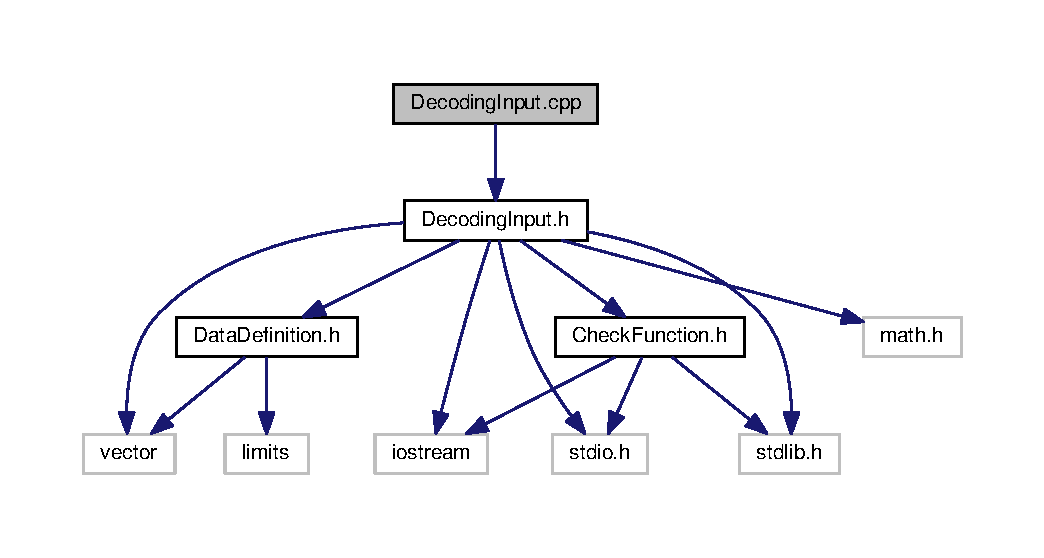
\includegraphics[width=350pt]{DecodingInput_8cpp__incl}
\end{center}
\end{figure}
\subsection*{Functions}
\begin{DoxyCompactItemize}
\item 
void \hyperlink{DecodingInput_8cpp_aa782eca5b098d797c8d30c74a72867ff}{compute\-Ind\-Matrix} (vector$<$ int $>$ input)
\item 
void \hyperlink{DecodingInput_8cpp_a19f422d53bf7ced4e3c7980cbdf76070}{compute\-Q\-Matrix} (int \hyperlink{ConflictGraph_8cpp_a2f6dbcf4fcf737ed9e4bcfbba6a961fa}{n\-\_\-utenti}, int $\ast$\hyperlink{ConflictGraph_8cpp_a1d12de4f14bfff1b963f424aac823fd5}{b\-\_\-chuncks})
\item 
void \hyperlink{DecodingInput_8cpp_a205ca4ba89c71b97219af118fe2c2780}{\-\_\-alloc\-Arrays} (int \hyperlink{ConflictGraph_8cpp_a2f6dbcf4fcf737ed9e4bcfbba6a961fa}{n\-\_\-utenti}, int $\ast$\hyperlink{ConflictGraph_8cpp_a1d12de4f14bfff1b963f424aac823fd5}{b\-\_\-chuncks}, int \hyperlink{ConflictGraph_8cpp_abd950309ddc65353a014b00c8c4a11b0}{m\-\_\-files})
\item 
\hyperlink{DataDefinition_8h_aa8ca5572763177379406da03176d0ef9}{data\-\_\-matrix} \hyperlink{DecodingInput_8cpp_adeb27f5ee8cd0559470e879c8d606800}{from\-Array\-To\-Matrix} (int \hyperlink{ConflictGraph_8cpp_abd950309ddc65353a014b00c8c4a11b0}{m\-\_\-files}, int $\ast$\hyperlink{ConflictGraph_8cpp_a1d12de4f14bfff1b963f424aac823fd5}{b\-\_\-chuncks}, vector$<$ int $>$ input)
\end{DoxyCompactItemize}
\subsection*{Variables}
\begin{DoxyCompactItemize}
\item 
int $\ast$$\ast$$\ast$ \hyperlink{DecodingInput_8cpp_a8c945a42c2fbc141ea28ec1348dbfb72}{Ind\-\_\-cache} = N\-U\-L\-L
\item 
int $\ast$ \hyperlink{DecodingInput_8cpp_abb03b7268b29a994143a1b4f62596c79}{Q\-\_\-demand} = N\-U\-L\-L
\item 
int $\ast$$\ast$ \hyperlink{DecodingInput_8cpp_a17a68ce598f88610e937f6efa48f2e27}{Q\-\_\-matrix} = N\-U\-L\-L
\end{DoxyCompactItemize}


\subsection{Detailed Description}
A file to decoding the input informations such as, probability, pre-\/filled cache... 

\subsection{Function Documentation}
\hypertarget{DecodingInput_8cpp_a205ca4ba89c71b97219af118fe2c2780}{\index{Decoding\-Input.\-cpp@{Decoding\-Input.\-cpp}!\-\_\-alloc\-Arrays@{\-\_\-alloc\-Arrays}}
\index{\-\_\-alloc\-Arrays@{\-\_\-alloc\-Arrays}!DecodingInput.cpp@{Decoding\-Input.\-cpp}}
\subsubsection[{\-\_\-alloc\-Arrays}]{\setlength{\rightskip}{0pt plus 5cm}void \-\_\-alloc\-Arrays (
\begin{DoxyParamCaption}
\item[{int}]{n\-\_\-utenti, }
\item[{int $\ast$}]{b\-\_\-chuncks, }
\item[{int}]{m\-\_\-files}
\end{DoxyParamCaption}
)}}\label{DecodingInput_8cpp_a205ca4ba89c71b97219af118fe2c2780}


Here is the call graph for this function\-:
\nopagebreak
\begin{figure}[H]
\begin{center}
\leavevmode
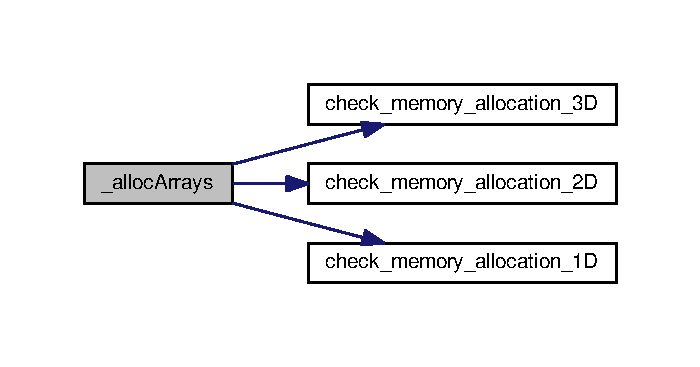
\includegraphics[width=336pt]{DecodingInput_8cpp_a205ca4ba89c71b97219af118fe2c2780_cgraph}
\end{center}
\end{figure}




Here is the caller graph for this function\-:
\nopagebreak
\begin{figure}[H]
\begin{center}
\leavevmode
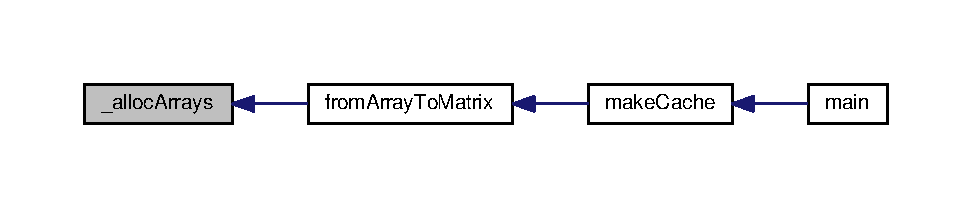
\includegraphics[width=350pt]{DecodingInput_8cpp_a205ca4ba89c71b97219af118fe2c2780_icgraph}
\end{center}
\end{figure}


\hypertarget{DecodingInput_8cpp_aa782eca5b098d797c8d30c74a72867ff}{\index{Decoding\-Input.\-cpp@{Decoding\-Input.\-cpp}!compute\-Ind\-Matrix@{compute\-Ind\-Matrix}}
\index{compute\-Ind\-Matrix@{compute\-Ind\-Matrix}!DecodingInput.cpp@{Decoding\-Input.\-cpp}}
\subsubsection[{compute\-Ind\-Matrix}]{\setlength{\rightskip}{0pt plus 5cm}void compute\-Ind\-Matrix (
\begin{DoxyParamCaption}
\item[{vector$<$ int $>$}]{input}
\end{DoxyParamCaption}
)}}\label{DecodingInput_8cpp_aa782eca5b098d797c8d30c74a72867ff}
This is a function that provide a compute the Ind cache matrix, this matrix is a binary matrix, Ind\mbox{[}i,j,k\mbox{]} = 0 if the user 'i' not have the chunk 'k' associated to file 'j' 

Here is the caller graph for this function\-:
\nopagebreak
\begin{figure}[H]
\begin{center}
\leavevmode
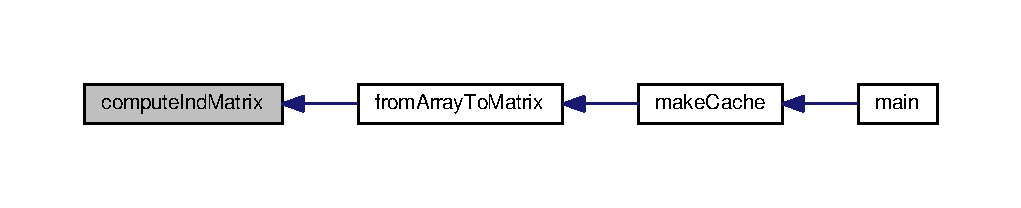
\includegraphics[width=350pt]{DecodingInput_8cpp_aa782eca5b098d797c8d30c74a72867ff_icgraph}
\end{center}
\end{figure}


\hypertarget{DecodingInput_8cpp_a19f422d53bf7ced4e3c7980cbdf76070}{\index{Decoding\-Input.\-cpp@{Decoding\-Input.\-cpp}!compute\-Q\-Matrix@{compute\-Q\-Matrix}}
\index{compute\-Q\-Matrix@{compute\-Q\-Matrix}!DecodingInput.cpp@{Decoding\-Input.\-cpp}}
\subsubsection[{compute\-Q\-Matrix}]{\setlength{\rightskip}{0pt plus 5cm}void compute\-Q\-Matrix (
\begin{DoxyParamCaption}
\item[{int}]{n\-\_\-utenti, }
\item[{int $\ast$}]{b\-\_\-chuncks}
\end{DoxyParamCaption}
)}}\label{DecodingInput_8cpp_a19f422d53bf7ced4e3c7980cbdf76070}
This is a function that provide a compute the Q matrix, this matrix is a binary matrix, Q\mbox{[}i,k\mbox{]} = 0 if the user 'i' have in cache the chunk 'k' related to files that he request 

Here is the caller graph for this function\-:
\nopagebreak
\begin{figure}[H]
\begin{center}
\leavevmode
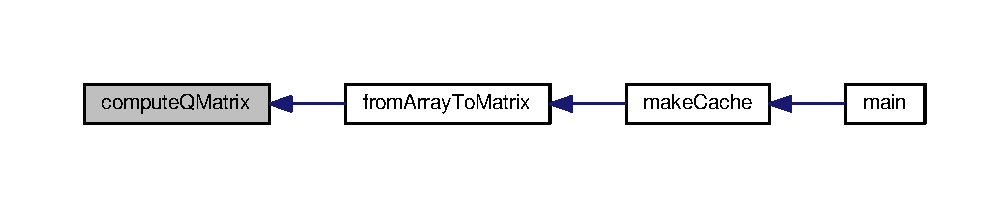
\includegraphics[width=350pt]{DecodingInput_8cpp_a19f422d53bf7ced4e3c7980cbdf76070_icgraph}
\end{center}
\end{figure}


\hypertarget{DecodingInput_8cpp_adeb27f5ee8cd0559470e879c8d606800}{\index{Decoding\-Input.\-cpp@{Decoding\-Input.\-cpp}!from\-Array\-To\-Matrix@{from\-Array\-To\-Matrix}}
\index{from\-Array\-To\-Matrix@{from\-Array\-To\-Matrix}!DecodingInput.cpp@{Decoding\-Input.\-cpp}}
\subsubsection[{from\-Array\-To\-Matrix}]{\setlength{\rightskip}{0pt plus 5cm}{\bf data\-\_\-matrix} from\-Array\-To\-Matrix (
\begin{DoxyParamCaption}
\item[{int}]{m\-\_\-files, }
\item[{int $\ast$}]{b\-\_\-chuncks, }
\item[{vector$<$ int $>$}]{input}
\end{DoxyParamCaption}
)}}\label{DecodingInput_8cpp_adeb27f5ee8cd0559470e879c8d606800}
Compute the cache binary matrix

Compute the binary matrix Q 

Here is the call graph for this function\-:
\nopagebreak
\begin{figure}[H]
\begin{center}
\leavevmode
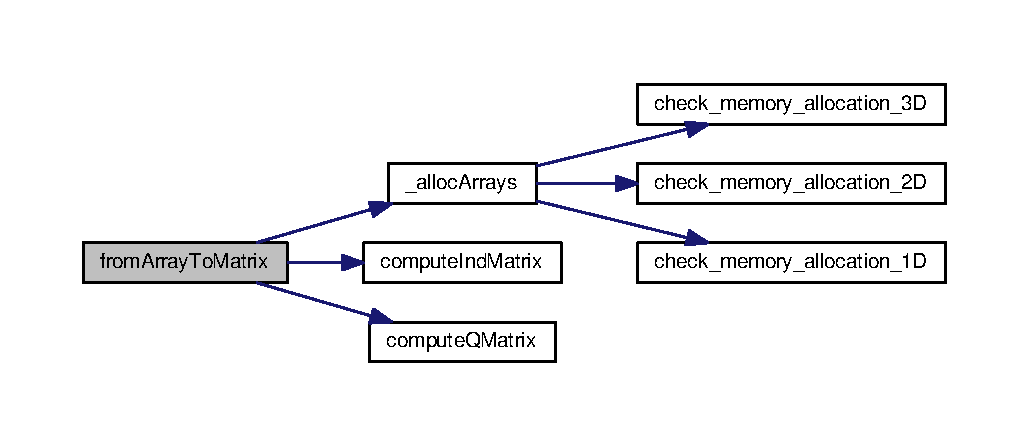
\includegraphics[width=350pt]{DecodingInput_8cpp_adeb27f5ee8cd0559470e879c8d606800_cgraph}
\end{center}
\end{figure}




Here is the caller graph for this function\-:
\nopagebreak
\begin{figure}[H]
\begin{center}
\leavevmode
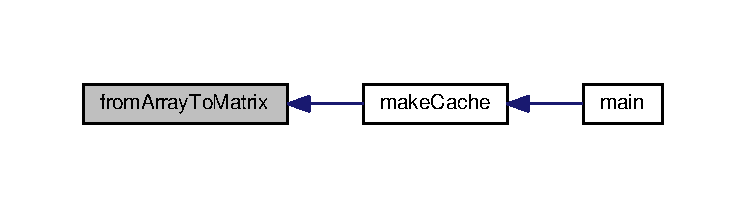
\includegraphics[width=350pt]{DecodingInput_8cpp_adeb27f5ee8cd0559470e879c8d606800_icgraph}
\end{center}
\end{figure}




\subsection{Variable Documentation}
\hypertarget{DecodingInput_8cpp_a8c945a42c2fbc141ea28ec1348dbfb72}{\index{Decoding\-Input.\-cpp@{Decoding\-Input.\-cpp}!Ind\-\_\-cache@{Ind\-\_\-cache}}
\index{Ind\-\_\-cache@{Ind\-\_\-cache}!DecodingInput.cpp@{Decoding\-Input.\-cpp}}
\subsubsection[{Ind\-\_\-cache}]{\setlength{\rightskip}{0pt plus 5cm}int$\ast$$\ast$$\ast$ Ind\-\_\-cache = N\-U\-L\-L}}\label{DecodingInput_8cpp_a8c945a42c2fbc141ea28ec1348dbfb72}
\hypertarget{DecodingInput_8cpp_abb03b7268b29a994143a1b4f62596c79}{\index{Decoding\-Input.\-cpp@{Decoding\-Input.\-cpp}!Q\-\_\-demand@{Q\-\_\-demand}}
\index{Q\-\_\-demand@{Q\-\_\-demand}!DecodingInput.cpp@{Decoding\-Input.\-cpp}}
\subsubsection[{Q\-\_\-demand}]{\setlength{\rightskip}{0pt plus 5cm}int$\ast$ Q\-\_\-demand = N\-U\-L\-L}}\label{DecodingInput_8cpp_abb03b7268b29a994143a1b4f62596c79}
\hypertarget{DecodingInput_8cpp_a17a68ce598f88610e937f6efa48f2e27}{\index{Decoding\-Input.\-cpp@{Decoding\-Input.\-cpp}!Q\-\_\-matrix@{Q\-\_\-matrix}}
\index{Q\-\_\-matrix@{Q\-\_\-matrix}!DecodingInput.cpp@{Decoding\-Input.\-cpp}}
\subsubsection[{Q\-\_\-matrix}]{\setlength{\rightskip}{0pt plus 5cm}int$\ast$$\ast$ Q\-\_\-matrix = N\-U\-L\-L}}\label{DecodingInput_8cpp_a17a68ce598f88610e937f6efa48f2e27}

\hypertarget{DecodingInput_8h}{\section{Decoding\-Input.\-h File Reference}
\label{DecodingInput_8h}\index{Decoding\-Input.\-h@{Decoding\-Input.\-h}}
}
{\ttfamily \#include $<$vector$>$}\\*
{\ttfamily \#include $<$iostream$>$}\\*
{\ttfamily \#include $<$stdio.\-h$>$}\\*
{\ttfamily \#include $<$stdlib.\-h$>$}\\*
{\ttfamily \#include $<$math.\-h$>$}\\*
{\ttfamily \#include \char`\"{}Check\-Function.\-h\char`\"{}}\\*
{\ttfamily \#include \char`\"{}Data\-Definition.\-h\char`\"{}}\\*
Include dependency graph for Decoding\-Input.\-h\-:
\nopagebreak
\begin{figure}[H]
\begin{center}
\leavevmode
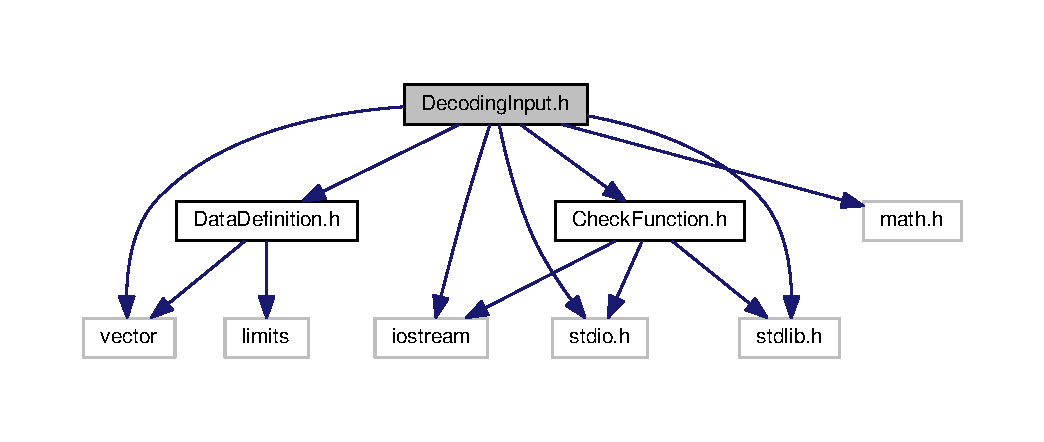
\includegraphics[width=350pt]{DecodingInput_8h__incl}
\end{center}
\end{figure}
This graph shows which files directly or indirectly include this file\-:
\nopagebreak
\begin{figure}[H]
\begin{center}
\leavevmode
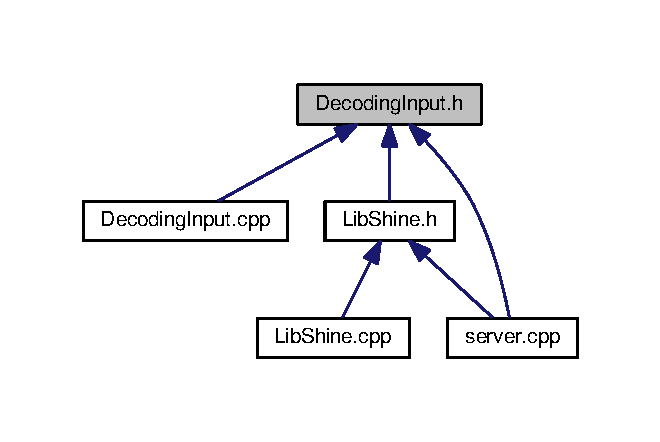
\includegraphics[width=317pt]{DecodingInput_8h__dep__incl}
\end{center}
\end{figure}
\subsection*{Functions}
\begin{DoxyCompactItemize}
\item 
void \hyperlink{DecodingInput_8h_ad13f010e00cde34fa1346751919d194d}{\-\_\-alloc\-Arrays} (int, int $\ast$, int)
\item 
\hyperlink{DataDefinition_8h_aa8ca5572763177379406da03176d0ef9}{data\-\_\-matrix} \hyperlink{DecodingInput_8h_a28260d6d34d82ba38bf908322d9b0254}{from\-Array\-To\-Matrix} (int, int $\ast$, vector$<$ int $>$)
\item 
void \hyperlink{DecodingInput_8h_a0fc3be48ee8a5a0acfc51421b906738f}{compute\-Q\-Matrix} (int, int $\ast$)
\item 
void \hyperlink{DecodingInput_8h_a72344c8082937dc8376238b437f63be6}{compute\-Ind\-Matrix} (vector$<$ int $>$)
\end{DoxyCompactItemize}


\subsection{Function Documentation}
\hypertarget{DecodingInput_8h_ad13f010e00cde34fa1346751919d194d}{\index{Decoding\-Input.\-h@{Decoding\-Input.\-h}!\-\_\-alloc\-Arrays@{\-\_\-alloc\-Arrays}}
\index{\-\_\-alloc\-Arrays@{\-\_\-alloc\-Arrays}!DecodingInput.h@{Decoding\-Input.\-h}}
\subsubsection[{\-\_\-alloc\-Arrays}]{\setlength{\rightskip}{0pt plus 5cm}void \-\_\-alloc\-Arrays (
\begin{DoxyParamCaption}
\item[{int}]{, }
\item[{int $\ast$}]{, }
\item[{int}]{}
\end{DoxyParamCaption}
)}}\label{DecodingInput_8h_ad13f010e00cde34fa1346751919d194d}


Here is the call graph for this function\-:
\nopagebreak
\begin{figure}[H]
\begin{center}
\leavevmode
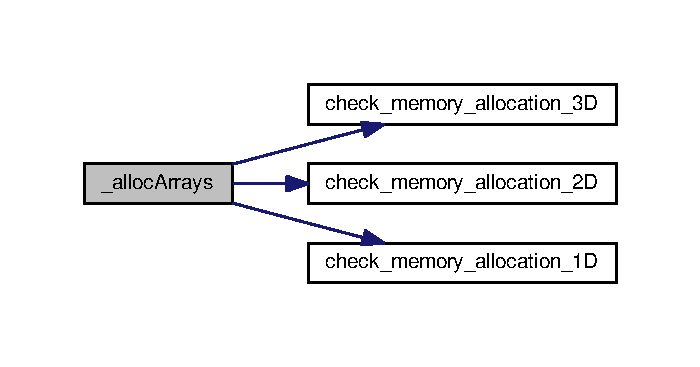
\includegraphics[width=336pt]{DecodingInput_8h_ad13f010e00cde34fa1346751919d194d_cgraph}
\end{center}
\end{figure}




Here is the caller graph for this function\-:
\nopagebreak
\begin{figure}[H]
\begin{center}
\leavevmode
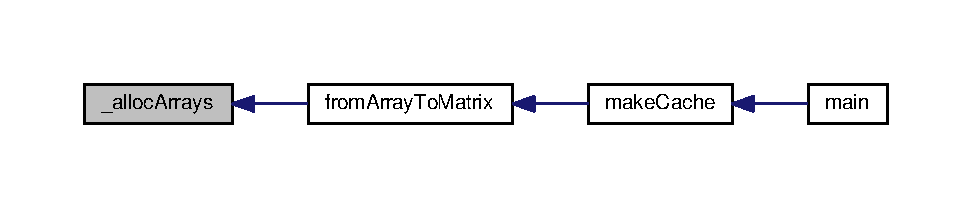
\includegraphics[width=350pt]{DecodingInput_8h_ad13f010e00cde34fa1346751919d194d_icgraph}
\end{center}
\end{figure}


\hypertarget{DecodingInput_8h_a72344c8082937dc8376238b437f63be6}{\index{Decoding\-Input.\-h@{Decoding\-Input.\-h}!compute\-Ind\-Matrix@{compute\-Ind\-Matrix}}
\index{compute\-Ind\-Matrix@{compute\-Ind\-Matrix}!DecodingInput.h@{Decoding\-Input.\-h}}
\subsubsection[{compute\-Ind\-Matrix}]{\setlength{\rightskip}{0pt plus 5cm}void compute\-Ind\-Matrix (
\begin{DoxyParamCaption}
\item[{vector$<$ int $>$}]{input}
\end{DoxyParamCaption}
)}}\label{DecodingInput_8h_a72344c8082937dc8376238b437f63be6}
This is a function that provide a compute the Ind cache matrix, this matrix is a binary matrix, Ind\mbox{[}i,j,k\mbox{]} = 0 if the user 'i' not have the chunk 'k' associated to file 'j' 

Here is the caller graph for this function\-:
\nopagebreak
\begin{figure}[H]
\begin{center}
\leavevmode
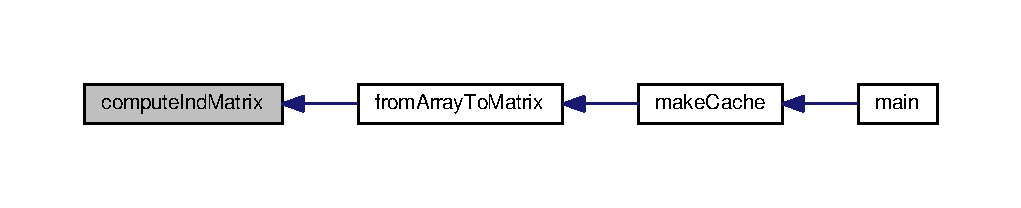
\includegraphics[width=350pt]{DecodingInput_8h_a72344c8082937dc8376238b437f63be6_icgraph}
\end{center}
\end{figure}


\hypertarget{DecodingInput_8h_a0fc3be48ee8a5a0acfc51421b906738f}{\index{Decoding\-Input.\-h@{Decoding\-Input.\-h}!compute\-Q\-Matrix@{compute\-Q\-Matrix}}
\index{compute\-Q\-Matrix@{compute\-Q\-Matrix}!DecodingInput.h@{Decoding\-Input.\-h}}
\subsubsection[{compute\-Q\-Matrix}]{\setlength{\rightskip}{0pt plus 5cm}void compute\-Q\-Matrix (
\begin{DoxyParamCaption}
\item[{int}]{n\-\_\-utenti, }
\item[{int $\ast$}]{b\-\_\-chuncks}
\end{DoxyParamCaption}
)}}\label{DecodingInput_8h_a0fc3be48ee8a5a0acfc51421b906738f}
This is a function that provide a compute the Q matrix, this matrix is a binary matrix, Q\mbox{[}i,k\mbox{]} = 0 if the user 'i' have in cache the chunk 'k' related to files that he request 

Here is the caller graph for this function\-:
\nopagebreak
\begin{figure}[H]
\begin{center}
\leavevmode
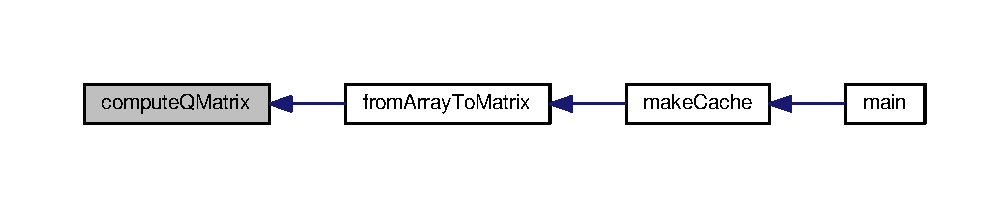
\includegraphics[width=350pt]{DecodingInput_8h_a0fc3be48ee8a5a0acfc51421b906738f_icgraph}
\end{center}
\end{figure}


\hypertarget{DecodingInput_8h_a28260d6d34d82ba38bf908322d9b0254}{\index{Decoding\-Input.\-h@{Decoding\-Input.\-h}!from\-Array\-To\-Matrix@{from\-Array\-To\-Matrix}}
\index{from\-Array\-To\-Matrix@{from\-Array\-To\-Matrix}!DecodingInput.h@{Decoding\-Input.\-h}}
\subsubsection[{from\-Array\-To\-Matrix}]{\setlength{\rightskip}{0pt plus 5cm}{\bf data\-\_\-matrix} from\-Array\-To\-Matrix (
\begin{DoxyParamCaption}
\item[{int}]{, }
\item[{int $\ast$}]{, }
\item[{vector$<$ int $>$}]{}
\end{DoxyParamCaption}
)}}\label{DecodingInput_8h_a28260d6d34d82ba38bf908322d9b0254}
Compute the cache binary matrix

Compute the binary matrix Q 

Here is the call graph for this function\-:
\nopagebreak
\begin{figure}[H]
\begin{center}
\leavevmode
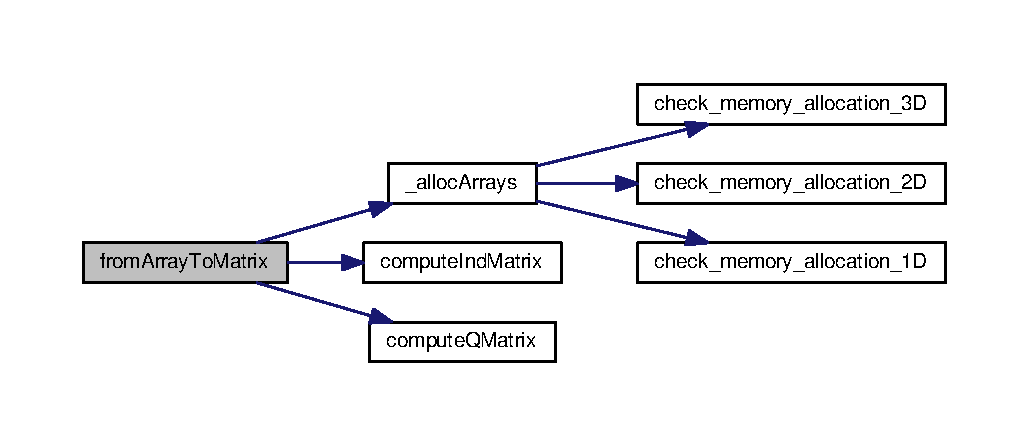
\includegraphics[width=350pt]{DecodingInput_8h_a28260d6d34d82ba38bf908322d9b0254_cgraph}
\end{center}
\end{figure}




Here is the caller graph for this function\-:
\nopagebreak
\begin{figure}[H]
\begin{center}
\leavevmode
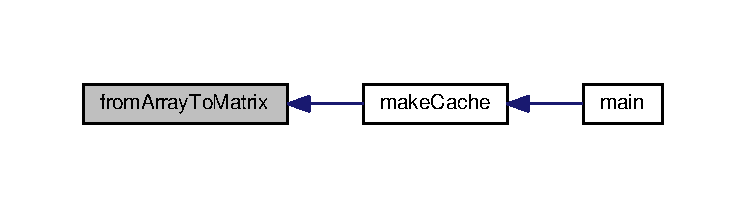
\includegraphics[width=350pt]{DecodingInput_8h_a28260d6d34d82ba38bf908322d9b0254_icgraph}
\end{center}
\end{figure}



\hypertarget{EnvironmentSetup_8cpp}{\section{Environment\-Setup.\-cpp File Reference}
\label{EnvironmentSetup_8cpp}\index{Environment\-Setup.\-cpp@{Environment\-Setup.\-cpp}}
}


A file to setup the environment when the server starts.  


{\ttfamily \#include \char`\"{}Environment\-Setup.\-h\char`\"{}}\\*
Include dependency graph for Environment\-Setup.\-cpp\-:
\nopagebreak
\begin{figure}[H]
\begin{center}
\leavevmode
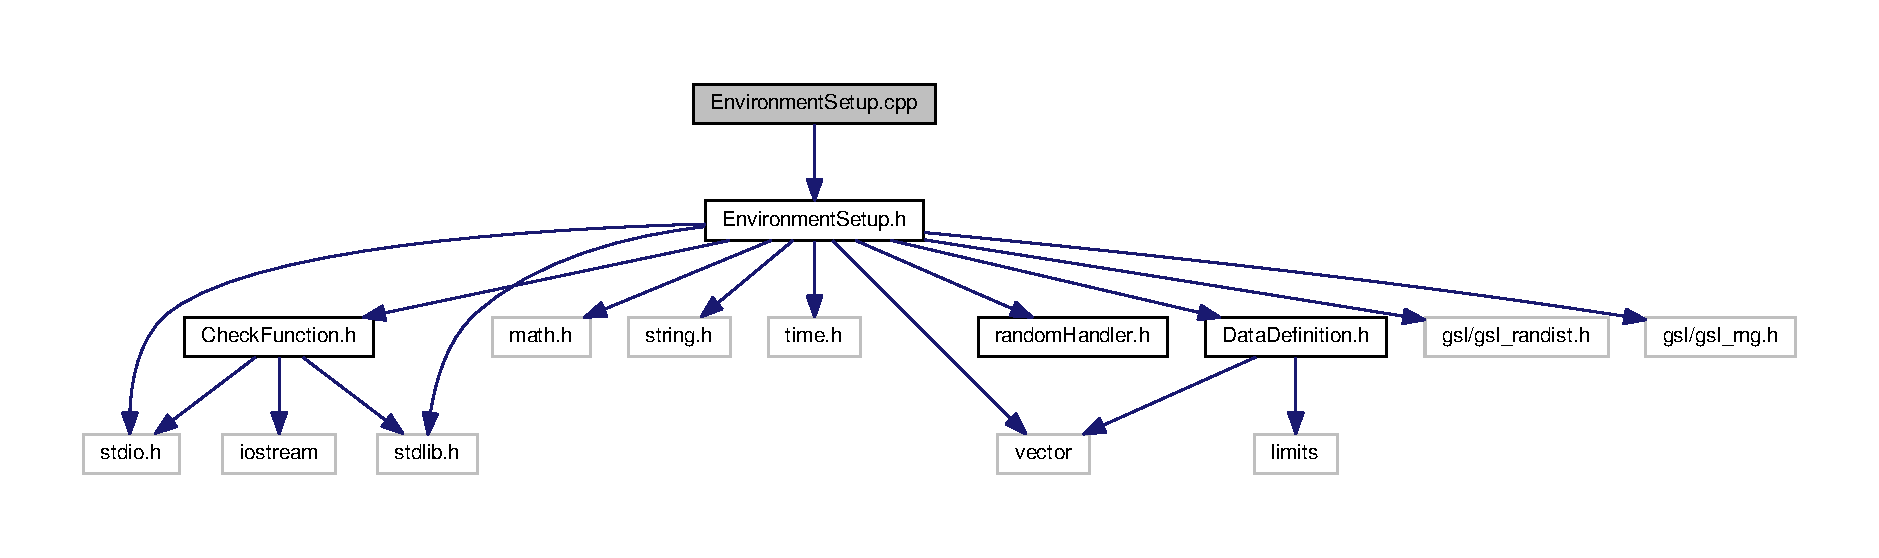
\includegraphics[width=350pt]{EnvironmentSetup_8cpp__incl}
\end{center}
\end{figure}
\subsection*{Functions}
\begin{DoxyCompactItemize}
\item 
void \hyperlink{EnvironmentSetup_8cpp_abaf06bc6f4c1bede056ea6b7ec94e05c}{random\-Q\-Vector} (double $\ast$$\ast$probs)
\item 
void \hyperlink{EnvironmentSetup_8cpp_a4d50fc0d1a9264291bfb35ec3175c4d9}{random\-Ind\-Matrix} (float memory\-\_\-discretizzata, int $\ast$$\ast$M, vector$<$ int $>$ \&input, int number\-\_\-of\-\_\-request, vector$<$ int $>$ memory\-\_\-per\-\_\-user)
\item 
void \hyperlink{EnvironmentSetup_8cpp_a8b78d1d7ffbdd78e9d0da690a2cf9ca4}{\-\_\-alloc\-Variables} ()
\item 
void \hyperlink{EnvironmentSetup_8cpp_ae60993fb259445fe13e581ae08ab1544}{\-\_\-dealloc\-Variables} ()
\item 
vector$<$ int $>$ \hyperlink{EnvironmentSetup_8cpp_ac6a9e71bb90d7953b32b3379e26b3de8}{set\-Environment} (int n\-\_\-utenti\-\_\-in, int m\-\_\-files\-\_\-in, int $\ast$b\-\_\-chuncks\-\_\-in, double $\ast$$\ast$probs, int $\ast$$\ast$M)
\end{DoxyCompactItemize}
\subsection*{Variables}
\begin{DoxyCompactItemize}
\item 
int \hyperlink{EnvironmentSetup_8cpp_ad60b7b31764dce9b0aca39b058497cd0}{n\-\_\-utenti\-\_\-env}
\item 
int \hyperlink{EnvironmentSetup_8cpp_abcfab90bc20db0b37162ffdc0553ef81}{m\-\_\-files\-\_\-env}
\item 
int $\ast$ \hyperlink{EnvironmentSetup_8cpp_a2855cde2dabfbb76bb70fb921659e731}{b\-\_\-chuncks\-\_\-env}
\item 
int $\ast$ \hyperlink{EnvironmentSetup_8cpp_adcf171e8a8853d501c3c5c06483611ce}{Q\-\_\-array} = N\-U\-L\-L
\end{DoxyCompactItemize}


\subsection{Detailed Description}
A file to setup the environment when the server starts. 

\subsection{Function Documentation}
\hypertarget{EnvironmentSetup_8cpp_a8b78d1d7ffbdd78e9d0da690a2cf9ca4}{\index{Environment\-Setup.\-cpp@{Environment\-Setup.\-cpp}!\-\_\-alloc\-Variables@{\-\_\-alloc\-Variables}}
\index{\-\_\-alloc\-Variables@{\-\_\-alloc\-Variables}!EnvironmentSetup.cpp@{Environment\-Setup.\-cpp}}
\subsubsection[{\-\_\-alloc\-Variables}]{\setlength{\rightskip}{0pt plus 5cm}void \-\_\-alloc\-Variables (
\begin{DoxyParamCaption}
{}
\end{DoxyParamCaption}
)}}\label{EnvironmentSetup_8cpp_a8b78d1d7ffbdd78e9d0da690a2cf9ca4}


Here is the call graph for this function\-:
\nopagebreak
\begin{figure}[H]
\begin{center}
\leavevmode
\includegraphics[width=348pt]{EnvironmentSetup_8cpp_a8b78d1d7ffbdd78e9d0da690a2cf9ca4_cgraph}
\end{center}
\end{figure}




Here is the caller graph for this function\-:
\nopagebreak
\begin{figure}[H]
\begin{center}
\leavevmode
\includegraphics[width=350pt]{EnvironmentSetup_8cpp_a8b78d1d7ffbdd78e9d0da690a2cf9ca4_icgraph}
\end{center}
\end{figure}


\hypertarget{EnvironmentSetup_8cpp_ae60993fb259445fe13e581ae08ab1544}{\index{Environment\-Setup.\-cpp@{Environment\-Setup.\-cpp}!\-\_\-dealloc\-Variables@{\-\_\-dealloc\-Variables}}
\index{\-\_\-dealloc\-Variables@{\-\_\-dealloc\-Variables}!EnvironmentSetup.cpp@{Environment\-Setup.\-cpp}}
\subsubsection[{\-\_\-dealloc\-Variables}]{\setlength{\rightskip}{0pt plus 5cm}void \-\_\-dealloc\-Variables (
\begin{DoxyParamCaption}
{}
\end{DoxyParamCaption}
)}}\label{EnvironmentSetup_8cpp_ae60993fb259445fe13e581ae08ab1544}


Here is the caller graph for this function\-:
\nopagebreak
\begin{figure}[H]
\begin{center}
\leavevmode
\includegraphics[width=350pt]{EnvironmentSetup_8cpp_ae60993fb259445fe13e581ae08ab1544_icgraph}
\end{center}
\end{figure}


\hypertarget{EnvironmentSetup_8cpp_a4d50fc0d1a9264291bfb35ec3175c4d9}{\index{Environment\-Setup.\-cpp@{Environment\-Setup.\-cpp}!random\-Ind\-Matrix@{random\-Ind\-Matrix}}
\index{random\-Ind\-Matrix@{random\-Ind\-Matrix}!EnvironmentSetup.cpp@{Environment\-Setup.\-cpp}}
\subsubsection[{random\-Ind\-Matrix}]{\setlength{\rightskip}{0pt plus 5cm}void random\-Ind\-Matrix (
\begin{DoxyParamCaption}
\item[{float}]{memory\-\_\-discretizzata, }
\item[{int $\ast$$\ast$}]{M, }
\item[{vector$<$ int $>$ \&}]{input, }
\item[{int}]{number\-\_\-of\-\_\-request, }
\item[{vector$<$ int $>$}]{memory\-\_\-per\-\_\-user}
\end{DoxyParamCaption}
)}}\label{EnvironmentSetup_8cpp_a4d50fc0d1a9264291bfb35ec3175c4d9}


Here is the call graph for this function\-:
\nopagebreak
\begin{figure}[H]
\begin{center}
\leavevmode
\includegraphics[width=350pt]{EnvironmentSetup_8cpp_a4d50fc0d1a9264291bfb35ec3175c4d9_cgraph}
\end{center}
\end{figure}




Here is the caller graph for this function\-:
\nopagebreak
\begin{figure}[H]
\begin{center}
\leavevmode
\includegraphics[width=350pt]{EnvironmentSetup_8cpp_a4d50fc0d1a9264291bfb35ec3175c4d9_icgraph}
\end{center}
\end{figure}


\hypertarget{EnvironmentSetup_8cpp_abaf06bc6f4c1bede056ea6b7ec94e05c}{\index{Environment\-Setup.\-cpp@{Environment\-Setup.\-cpp}!random\-Q\-Vector@{random\-Q\-Vector}}
\index{random\-Q\-Vector@{random\-Q\-Vector}!EnvironmentSetup.cpp@{Environment\-Setup.\-cpp}}
\subsubsection[{random\-Q\-Vector}]{\setlength{\rightskip}{0pt plus 5cm}void random\-Q\-Vector (
\begin{DoxyParamCaption}
\item[{double $\ast$$\ast$}]{probs}
\end{DoxyParamCaption}
)}}\label{EnvironmentSetup_8cpp_abaf06bc6f4c1bede056ea6b7ec94e05c}


Here is the caller graph for this function\-:
\nopagebreak
\begin{figure}[H]
\begin{center}
\leavevmode
\includegraphics[width=350pt]{EnvironmentSetup_8cpp_abaf06bc6f4c1bede056ea6b7ec94e05c_icgraph}
\end{center}
\end{figure}


\hypertarget{EnvironmentSetup_8cpp_ac6a9e71bb90d7953b32b3379e26b3de8}{\index{Environment\-Setup.\-cpp@{Environment\-Setup.\-cpp}!set\-Environment@{set\-Environment}}
\index{set\-Environment@{set\-Environment}!EnvironmentSetup.cpp@{Environment\-Setup.\-cpp}}
\subsubsection[{set\-Environment}]{\setlength{\rightskip}{0pt plus 5cm}vector$<$int$>$ set\-Environment (
\begin{DoxyParamCaption}
\item[{int}]{n\-\_\-utenti\-\_\-in, }
\item[{int}]{m\-\_\-files\-\_\-in, }
\item[{int $\ast$}]{b\-\_\-chuncks\-\_\-in, }
\item[{double $\ast$$\ast$}]{probs, }
\item[{int $\ast$$\ast$}]{M}
\end{DoxyParamCaption}
)}}\label{EnvironmentSetup_8cpp_ac6a9e71bb90d7953b32b3379e26b3de8}


Here is the call graph for this function\-:
\nopagebreak
\begin{figure}[H]
\begin{center}
\leavevmode
\includegraphics[width=350pt]{EnvironmentSetup_8cpp_ac6a9e71bb90d7953b32b3379e26b3de8_cgraph}
\end{center}
\end{figure}




Here is the caller graph for this function\-:
\nopagebreak
\begin{figure}[H]
\begin{center}
\leavevmode
\includegraphics[width=346pt]{EnvironmentSetup_8cpp_ac6a9e71bb90d7953b32b3379e26b3de8_icgraph}
\end{center}
\end{figure}




\subsection{Variable Documentation}
\hypertarget{EnvironmentSetup_8cpp_a2855cde2dabfbb76bb70fb921659e731}{\index{Environment\-Setup.\-cpp@{Environment\-Setup.\-cpp}!b\-\_\-chuncks\-\_\-env@{b\-\_\-chuncks\-\_\-env}}
\index{b\-\_\-chuncks\-\_\-env@{b\-\_\-chuncks\-\_\-env}!EnvironmentSetup.cpp@{Environment\-Setup.\-cpp}}
\subsubsection[{b\-\_\-chuncks\-\_\-env}]{\setlength{\rightskip}{0pt plus 5cm}int$\ast$ b\-\_\-chuncks\-\_\-env}}\label{EnvironmentSetup_8cpp_a2855cde2dabfbb76bb70fb921659e731}
\hypertarget{EnvironmentSetup_8cpp_abcfab90bc20db0b37162ffdc0553ef81}{\index{Environment\-Setup.\-cpp@{Environment\-Setup.\-cpp}!m\-\_\-files\-\_\-env@{m\-\_\-files\-\_\-env}}
\index{m\-\_\-files\-\_\-env@{m\-\_\-files\-\_\-env}!EnvironmentSetup.cpp@{Environment\-Setup.\-cpp}}
\subsubsection[{m\-\_\-files\-\_\-env}]{\setlength{\rightskip}{0pt plus 5cm}int m\-\_\-files\-\_\-env}}\label{EnvironmentSetup_8cpp_abcfab90bc20db0b37162ffdc0553ef81}
\hypertarget{EnvironmentSetup_8cpp_ad60b7b31764dce9b0aca39b058497cd0}{\index{Environment\-Setup.\-cpp@{Environment\-Setup.\-cpp}!n\-\_\-utenti\-\_\-env@{n\-\_\-utenti\-\_\-env}}
\index{n\-\_\-utenti\-\_\-env@{n\-\_\-utenti\-\_\-env}!EnvironmentSetup.cpp@{Environment\-Setup.\-cpp}}
\subsubsection[{n\-\_\-utenti\-\_\-env}]{\setlength{\rightskip}{0pt plus 5cm}int n\-\_\-utenti\-\_\-env}}\label{EnvironmentSetup_8cpp_ad60b7b31764dce9b0aca39b058497cd0}
\hypertarget{EnvironmentSetup_8cpp_adcf171e8a8853d501c3c5c06483611ce}{\index{Environment\-Setup.\-cpp@{Environment\-Setup.\-cpp}!Q\-\_\-array@{Q\-\_\-array}}
\index{Q\-\_\-array@{Q\-\_\-array}!EnvironmentSetup.cpp@{Environment\-Setup.\-cpp}}
\subsubsection[{Q\-\_\-array}]{\setlength{\rightskip}{0pt plus 5cm}int$\ast$ Q\-\_\-array = N\-U\-L\-L}}\label{EnvironmentSetup_8cpp_adcf171e8a8853d501c3c5c06483611ce}

\hypertarget{EnvironmentSetup_8h}{\section{Environment\-Setup.\-h File Reference}
\label{EnvironmentSetup_8h}\index{Environment\-Setup.\-h@{Environment\-Setup.\-h}}
}
{\ttfamily \#include $<$vector$>$}\\*
{\ttfamily \#include $<$stdio.\-h$>$}\\*
{\ttfamily \#include $<$stdlib.\-h$>$}\\*
{\ttfamily \#include $<$math.\-h$>$}\\*
{\ttfamily \#include $<$string.\-h$>$}\\*
{\ttfamily \#include $<$time.\-h$>$}\\*
{\ttfamily \#include \char`\"{}Check\-Function.\-h\char`\"{}}\\*
{\ttfamily \#include \char`\"{}random\-Handler.\-h\char`\"{}}\\*
{\ttfamily \#include \char`\"{}Data\-Definition.\-h\char`\"{}}\\*
{\ttfamily \#include $<$gsl/gsl\-\_\-randist.\-h$>$}\\*
{\ttfamily \#include $<$gsl/gsl\-\_\-rng.\-h$>$}\\*
Include dependency graph for Environment\-Setup.\-h\-:
\nopagebreak
\begin{figure}[H]
\begin{center}
\leavevmode
\includegraphics[width=350pt]{EnvironmentSetup_8h__incl}
\end{center}
\end{figure}
This graph shows which files directly or indirectly include this file\-:
\nopagebreak
\begin{figure}[H]
\begin{center}
\leavevmode
\includegraphics[width=335pt]{EnvironmentSetup_8h__dep__incl}
\end{center}
\end{figure}
\subsection*{Functions}
\begin{DoxyCompactItemize}
\item 
void \hyperlink{EnvironmentSetup_8h_a86173f356060a9a97d780eef2b690819}{random\-Ind\-Matrix} (float, int $\ast$$\ast$, vector$<$ int $>$ \&, int, vector$<$ int $>$)
\item 
void \hyperlink{EnvironmentSetup_8h_a85784dacc323765a4ca27b77159be069}{random\-Q\-Vector} (double $\ast$$\ast$)
\item 
void \hyperlink{EnvironmentSetup_8h_a8b78d1d7ffbdd78e9d0da690a2cf9ca4}{\-\_\-alloc\-Variables} ()
\item 
void \hyperlink{EnvironmentSetup_8h_ae60993fb259445fe13e581ae08ab1544}{\-\_\-dealloc\-Variables} ()
\item 
vector$<$ int $>$ \hyperlink{EnvironmentSetup_8h_a9622719f219854837b4710801b770278}{set\-Environment} (int, int, int $\ast$, double $\ast$$\ast$, int $\ast$$\ast$)
\end{DoxyCompactItemize}


\subsection{Function Documentation}
\hypertarget{EnvironmentSetup_8h_a8b78d1d7ffbdd78e9d0da690a2cf9ca4}{\index{Environment\-Setup.\-h@{Environment\-Setup.\-h}!\-\_\-alloc\-Variables@{\-\_\-alloc\-Variables}}
\index{\-\_\-alloc\-Variables@{\-\_\-alloc\-Variables}!EnvironmentSetup.h@{Environment\-Setup.\-h}}
\subsubsection[{\-\_\-alloc\-Variables}]{\setlength{\rightskip}{0pt plus 5cm}void \-\_\-alloc\-Variables (
\begin{DoxyParamCaption}
{}
\end{DoxyParamCaption}
)}}\label{EnvironmentSetup_8h_a8b78d1d7ffbdd78e9d0da690a2cf9ca4}


Here is the call graph for this function\-:
\nopagebreak
\begin{figure}[H]
\begin{center}
\leavevmode
\includegraphics[width=348pt]{EnvironmentSetup_8h_a8b78d1d7ffbdd78e9d0da690a2cf9ca4_cgraph}
\end{center}
\end{figure}




Here is the caller graph for this function\-:
\nopagebreak
\begin{figure}[H]
\begin{center}
\leavevmode
\includegraphics[width=350pt]{EnvironmentSetup_8h_a8b78d1d7ffbdd78e9d0da690a2cf9ca4_icgraph}
\end{center}
\end{figure}


\hypertarget{EnvironmentSetup_8h_ae60993fb259445fe13e581ae08ab1544}{\index{Environment\-Setup.\-h@{Environment\-Setup.\-h}!\-\_\-dealloc\-Variables@{\-\_\-dealloc\-Variables}}
\index{\-\_\-dealloc\-Variables@{\-\_\-dealloc\-Variables}!EnvironmentSetup.h@{Environment\-Setup.\-h}}
\subsubsection[{\-\_\-dealloc\-Variables}]{\setlength{\rightskip}{0pt plus 5cm}void \-\_\-dealloc\-Variables (
\begin{DoxyParamCaption}
{}
\end{DoxyParamCaption}
)}}\label{EnvironmentSetup_8h_ae60993fb259445fe13e581ae08ab1544}


Here is the caller graph for this function\-:
\nopagebreak
\begin{figure}[H]
\begin{center}
\leavevmode
\includegraphics[width=350pt]{EnvironmentSetup_8h_ae60993fb259445fe13e581ae08ab1544_icgraph}
\end{center}
\end{figure}


\hypertarget{EnvironmentSetup_8h_a86173f356060a9a97d780eef2b690819}{\index{Environment\-Setup.\-h@{Environment\-Setup.\-h}!random\-Ind\-Matrix@{random\-Ind\-Matrix}}
\index{random\-Ind\-Matrix@{random\-Ind\-Matrix}!EnvironmentSetup.h@{Environment\-Setup.\-h}}
\subsubsection[{random\-Ind\-Matrix}]{\setlength{\rightskip}{0pt plus 5cm}void random\-Ind\-Matrix (
\begin{DoxyParamCaption}
\item[{float}]{, }
\item[{int $\ast$$\ast$}]{, }
\item[{vector$<$ int $>$ \&}]{, }
\item[{int}]{, }
\item[{vector$<$ int $>$}]{}
\end{DoxyParamCaption}
)}}\label{EnvironmentSetup_8h_a86173f356060a9a97d780eef2b690819}


Here is the call graph for this function\-:
\nopagebreak
\begin{figure}[H]
\begin{center}
\leavevmode
\includegraphics[width=350pt]{EnvironmentSetup_8h_a86173f356060a9a97d780eef2b690819_cgraph}
\end{center}
\end{figure}




Here is the caller graph for this function\-:
\nopagebreak
\begin{figure}[H]
\begin{center}
\leavevmode
\includegraphics[width=350pt]{EnvironmentSetup_8h_a86173f356060a9a97d780eef2b690819_icgraph}
\end{center}
\end{figure}


\hypertarget{EnvironmentSetup_8h_a85784dacc323765a4ca27b77159be069}{\index{Environment\-Setup.\-h@{Environment\-Setup.\-h}!random\-Q\-Vector@{random\-Q\-Vector}}
\index{random\-Q\-Vector@{random\-Q\-Vector}!EnvironmentSetup.h@{Environment\-Setup.\-h}}
\subsubsection[{random\-Q\-Vector}]{\setlength{\rightskip}{0pt plus 5cm}void random\-Q\-Vector (
\begin{DoxyParamCaption}
\item[{double $\ast$$\ast$}]{}
\end{DoxyParamCaption}
)}}\label{EnvironmentSetup_8h_a85784dacc323765a4ca27b77159be069}


Here is the caller graph for this function\-:
\nopagebreak
\begin{figure}[H]
\begin{center}
\leavevmode
\includegraphics[width=350pt]{EnvironmentSetup_8h_a85784dacc323765a4ca27b77159be069_icgraph}
\end{center}
\end{figure}


\hypertarget{EnvironmentSetup_8h_a9622719f219854837b4710801b770278}{\index{Environment\-Setup.\-h@{Environment\-Setup.\-h}!set\-Environment@{set\-Environment}}
\index{set\-Environment@{set\-Environment}!EnvironmentSetup.h@{Environment\-Setup.\-h}}
\subsubsection[{set\-Environment}]{\setlength{\rightskip}{0pt plus 5cm}vector$<$int$>$ set\-Environment (
\begin{DoxyParamCaption}
\item[{int}]{, }
\item[{int}]{, }
\item[{int $\ast$}]{, }
\item[{double $\ast$$\ast$}]{, }
\item[{int $\ast$$\ast$}]{}
\end{DoxyParamCaption}
)}}\label{EnvironmentSetup_8h_a9622719f219854837b4710801b770278}


Here is the call graph for this function\-:
\nopagebreak
\begin{figure}[H]
\begin{center}
\leavevmode
\includegraphics[width=350pt]{EnvironmentSetup_8h_a9622719f219854837b4710801b770278_cgraph}
\end{center}
\end{figure}




Here is the caller graph for this function\-:
\nopagebreak
\begin{figure}[H]
\begin{center}
\leavevmode
\includegraphics[width=346pt]{EnvironmentSetup_8h_a9622719f219854837b4710801b770278_icgraph}
\end{center}
\end{figure}



\hypertarget{grasp_8cpp}{\section{grasp.\-cpp File Reference}
\label{grasp_8cpp}\index{grasp.\-cpp@{grasp.\-cpp}}
}


A file to perform the grasp algorthm.  


{\ttfamily \#include \char`\"{}grasp.\-h\char`\"{}}\\*
Include dependency graph for grasp.\-cpp\-:
\nopagebreak
\begin{figure}[H]
\begin{center}
\leavevmode
\includegraphics[width=350pt]{grasp_8cpp__incl}
\end{center}
\end{figure}
\subsection*{Functions}
\begin{DoxyCompactItemize}
\item 
void \hyperlink{grasp_8cpp_a126590b25b2890594214115a21ccb1b3}{grasp\-Process} ()
\item 
void \hyperlink{grasp_8cpp_add7bcf8b26bd5a2d232797368fa48d89}{run\-Grasp} ()
\item 
int $\ast$ \hyperlink{grasp_8cpp_a5cc6e669bfa130d1dcf3724422c94a54}{construct\-Greedy\-Randomized\-Solution} (int $\ast$fo, float alpha)
\item 
\hyperlink{DataDefinition_8h_a8c4793b470f20960e0647bcb528a171b}{R\-C\-L\-\_\-\-L\-I\-S\-T} $\ast$ \hyperlink{grasp_8cpp_a6f1c1271ab34597c22c4b7a2d25328a3}{make\-R\-C\-L} (float alpha, int $\ast$n\-\_\-rcl, int $\ast$sol)
\item 
int $\ast$ \hyperlink{grasp_8cpp_af5940778e8e7e9d5c37e9e1510a8851d}{local\-Search} (int $\ast$sol, int $\ast$fo)
\item 
void \hyperlink{grasp_8cpp_aceacf4aaf6cf419efe16a5c077f363a6}{check\-Constraints} (int $\ast$sol)
\item 
int \hyperlink{grasp_8cpp_afcfa843d43b4171385e2a18b6ec288be}{get\-Color} (\hyperlink{DataDefinition_8h_a17b26c913a8eb52ca9efdc06681981b7}{N\-O\-D\-E} $\ast$node, int $\ast$fo, int $\ast$sol)
\item 
void \hyperlink{grasp_8cpp_a8b702a9434f7145e69ce372fb712171e}{create\-Graph} (\hyperlink{DataDefinition_8h_a1601a7ee6f4213e7d70430cefa083def}{cf\-\_\-data} \hyperlink{server_8cpp_a7304f2f0c01460ea55ddd50e50918007}{output\-For\-Coloring})
\item 
int $\ast$ \hyperlink{grasp_8cpp_af11c331e2214bc02a7839fdde8c69183}{grasp\-Graph\-Coloring} (int max\-Iter, \hyperlink{DataDefinition_8h_a1601a7ee6f4213e7d70430cefa083def}{cf\-\_\-data} \hyperlink{server_8cpp_a7304f2f0c01460ea55ddd50e50918007}{output\-For\-Coloring}, int $\ast$\hyperlink{server_8cpp_a08ddc6ed3452290d5165e02bbe46d08b}{n\-\_\-col})
\end{DoxyCompactItemize}
\subsection*{Variables}
\begin{DoxyCompactItemize}
\item 
int \hyperlink{grasp_8cpp_aee3411655ef6bb273aec80d1ca9f6094}{n\-\_\-nodes}
\item 
int \hyperlink{grasp_8cpp_aa9bc6f802d505dd94ea7d9414f304200}{m\-\_\-edges}
\item 
int \hyperlink{grasp_8cpp_a8426849406ea58f92d7bd358a9f97b15}{fo\-\_\-star}
\item 
int \hyperlink{grasp_8cpp_adfed55b92ded4adea8686fe2014f85cb}{max\-Iterations}
\item 
int \hyperlink{grasp_8cpp_ae79c2acd1a014de0ff504f69b0194937}{descending}
\item 
\hyperlink{DataDefinition_8h_a17b26c913a8eb52ca9efdc06681981b7}{N\-O\-D\-E} $\ast$ \hyperlink{grasp_8cpp_a310ee5a2a3e67e88576d1cd5788006fc}{nodi\-\_\-grafo} = N\-U\-L\-L
\item 
int $\ast$ \hyperlink{grasp_8cpp_ad0307bc9a52785a6a43007325d48e878}{sol\-\_\-star} = N\-U\-L\-L
\end{DoxyCompactItemize}


\subsection{Detailed Description}
A file to perform the grasp algorthm. 

\subsection{Function Documentation}
\hypertarget{grasp_8cpp_aceacf4aaf6cf419efe16a5c077f363a6}{\index{grasp.\-cpp@{grasp.\-cpp}!check\-Constraints@{check\-Constraints}}
\index{check\-Constraints@{check\-Constraints}!grasp.cpp@{grasp.\-cpp}}
\subsubsection[{check\-Constraints}]{\setlength{\rightskip}{0pt plus 5cm}void check\-Constraints (
\begin{DoxyParamCaption}
\item[{int $\ast$}]{sol}
\end{DoxyParamCaption}
)}}\label{grasp_8cpp_aceacf4aaf6cf419efe16a5c077f363a6}


Here is the caller graph for this function\-:
\nopagebreak
\begin{figure}[H]
\begin{center}
\leavevmode
\includegraphics[width=350pt]{grasp_8cpp_aceacf4aaf6cf419efe16a5c077f363a6_icgraph}
\end{center}
\end{figure}


\hypertarget{grasp_8cpp_a5cc6e669bfa130d1dcf3724422c94a54}{\index{grasp.\-cpp@{grasp.\-cpp}!construct\-Greedy\-Randomized\-Solution@{construct\-Greedy\-Randomized\-Solution}}
\index{construct\-Greedy\-Randomized\-Solution@{construct\-Greedy\-Randomized\-Solution}!grasp.cpp@{grasp.\-cpp}}
\subsubsection[{construct\-Greedy\-Randomized\-Solution}]{\setlength{\rightskip}{0pt plus 5cm}int$\ast$ construct\-Greedy\-Randomized\-Solution (
\begin{DoxyParamCaption}
\item[{int $\ast$}]{fo, }
\item[{float}]{alpha}
\end{DoxyParamCaption}
)}}\label{grasp_8cpp_a5cc6e669bfa130d1dcf3724422c94a54}
This function provide to create an admissible solution 

Here is the call graph for this function\-:
\nopagebreak
\begin{figure}[H]
\begin{center}
\leavevmode
\includegraphics[width=350pt]{grasp_8cpp_a5cc6e669bfa130d1dcf3724422c94a54_cgraph}
\end{center}
\end{figure}




Here is the caller graph for this function\-:
\nopagebreak
\begin{figure}[H]
\begin{center}
\leavevmode
\includegraphics[width=350pt]{grasp_8cpp_a5cc6e669bfa130d1dcf3724422c94a54_icgraph}
\end{center}
\end{figure}


\hypertarget{grasp_8cpp_a8b702a9434f7145e69ce372fb712171e}{\index{grasp.\-cpp@{grasp.\-cpp}!create\-Graph@{create\-Graph}}
\index{create\-Graph@{create\-Graph}!grasp.cpp@{grasp.\-cpp}}
\subsubsection[{create\-Graph}]{\setlength{\rightskip}{0pt plus 5cm}void create\-Graph (
\begin{DoxyParamCaption}
\item[{{\bf cf\-\_\-data}}]{output\-For\-Coloring}
\end{DoxyParamCaption}
)}}\label{grasp_8cpp_a8b702a9434f7145e69ce372fb712171e}


Here is the caller graph for this function\-:
\nopagebreak
\begin{figure}[H]
\begin{center}
\leavevmode
\includegraphics[width=350pt]{grasp_8cpp_a8b702a9434f7145e69ce372fb712171e_icgraph}
\end{center}
\end{figure}


\hypertarget{grasp_8cpp_afcfa843d43b4171385e2a18b6ec288be}{\index{grasp.\-cpp@{grasp.\-cpp}!get\-Color@{get\-Color}}
\index{get\-Color@{get\-Color}!grasp.cpp@{grasp.\-cpp}}
\subsubsection[{get\-Color}]{\setlength{\rightskip}{0pt plus 5cm}int get\-Color (
\begin{DoxyParamCaption}
\item[{{\bf N\-O\-D\-E} $\ast$}]{node, }
\item[{int $\ast$}]{fo, }
\item[{int $\ast$}]{sol}
\end{DoxyParamCaption}
)}}\label{grasp_8cpp_afcfa843d43b4171385e2a18b6ec288be}
This function identifies, in according to the node's neighborhood, the color that can be associated to the node 

Here is the caller graph for this function\-:
\nopagebreak
\begin{figure}[H]
\begin{center}
\leavevmode
\includegraphics[width=350pt]{grasp_8cpp_afcfa843d43b4171385e2a18b6ec288be_icgraph}
\end{center}
\end{figure}


\hypertarget{grasp_8cpp_af11c331e2214bc02a7839fdde8c69183}{\index{grasp.\-cpp@{grasp.\-cpp}!grasp\-Graph\-Coloring@{grasp\-Graph\-Coloring}}
\index{grasp\-Graph\-Coloring@{grasp\-Graph\-Coloring}!grasp.cpp@{grasp.\-cpp}}
\subsubsection[{grasp\-Graph\-Coloring}]{\setlength{\rightskip}{0pt plus 5cm}int$\ast$ grasp\-Graph\-Coloring (
\begin{DoxyParamCaption}
\item[{int}]{max\-Iter, }
\item[{{\bf cf\-\_\-data}}]{output\-For\-Coloring, }
\item[{int $\ast$}]{n\-\_\-col}
\end{DoxyParamCaption}
)}}\label{grasp_8cpp_af11c331e2214bc02a7839fdde8c69183}
Main Function -\/ Input\-: Max Numbers Of G\-R\-A\-S\-P's Iterations 

Here is the call graph for this function\-:
\nopagebreak
\begin{figure}[H]
\begin{center}
\leavevmode
\includegraphics[width=350pt]{grasp_8cpp_af11c331e2214bc02a7839fdde8c69183_cgraph}
\end{center}
\end{figure}




Here is the caller graph for this function\-:
\nopagebreak
\begin{figure}[H]
\begin{center}
\leavevmode
\includegraphics[width=350pt]{grasp_8cpp_af11c331e2214bc02a7839fdde8c69183_icgraph}
\end{center}
\end{figure}


\hypertarget{grasp_8cpp_a126590b25b2890594214115a21ccb1b3}{\index{grasp.\-cpp@{grasp.\-cpp}!grasp\-Process@{grasp\-Process}}
\index{grasp\-Process@{grasp\-Process}!grasp.cpp@{grasp.\-cpp}}
\subsubsection[{grasp\-Process}]{\setlength{\rightskip}{0pt plus 5cm}void grasp\-Process (
\begin{DoxyParamCaption}
{}
\end{DoxyParamCaption}
)}}\label{grasp_8cpp_a126590b25b2890594214115a21ccb1b3}


Here is the call graph for this function\-:
\nopagebreak
\begin{figure}[H]
\begin{center}
\leavevmode
\includegraphics[width=350pt]{grasp_8cpp_a126590b25b2890594214115a21ccb1b3_cgraph}
\end{center}
\end{figure}




Here is the caller graph for this function\-:
\nopagebreak
\begin{figure}[H]
\begin{center}
\leavevmode
\includegraphics[width=350pt]{grasp_8cpp_a126590b25b2890594214115a21ccb1b3_icgraph}
\end{center}
\end{figure}


\hypertarget{grasp_8cpp_af5940778e8e7e9d5c37e9e1510a8851d}{\index{grasp.\-cpp@{grasp.\-cpp}!local\-Search@{local\-Search}}
\index{local\-Search@{local\-Search}!grasp.cpp@{grasp.\-cpp}}
\subsubsection[{local\-Search}]{\setlength{\rightskip}{0pt plus 5cm}int$\ast$ local\-Search (
\begin{DoxyParamCaption}
\item[{int $\ast$}]{sol, }
\item[{int $\ast$}]{fo}
\end{DoxyParamCaption}
)}}\label{grasp_8cpp_af5940778e8e7e9d5c37e9e1510a8851d}
This function try to improve the current solution. This procedure try to decrese the number of color utilized 

Here is the caller graph for this function\-:
\nopagebreak
\begin{figure}[H]
\begin{center}
\leavevmode
\includegraphics[width=350pt]{grasp_8cpp_af5940778e8e7e9d5c37e9e1510a8851d_icgraph}
\end{center}
\end{figure}


\hypertarget{grasp_8cpp_a6f1c1271ab34597c22c4b7a2d25328a3}{\index{grasp.\-cpp@{grasp.\-cpp}!make\-R\-C\-L@{make\-R\-C\-L}}
\index{make\-R\-C\-L@{make\-R\-C\-L}!grasp.cpp@{grasp.\-cpp}}
\subsubsection[{make\-R\-C\-L}]{\setlength{\rightskip}{0pt plus 5cm}{\bf R\-C\-L\-\_\-\-L\-I\-S\-T}$\ast$ make\-R\-C\-L (
\begin{DoxyParamCaption}
\item[{float}]{alpha, }
\item[{int $\ast$}]{n\-\_\-rcl, }
\item[{int $\ast$}]{sol}
\end{DoxyParamCaption}
)}}\label{grasp_8cpp_a6f1c1271ab34597c22c4b7a2d25328a3}
This function provide to create a Restricted Candidates List 

Here is the caller graph for this function\-:
\nopagebreak
\begin{figure}[H]
\begin{center}
\leavevmode
\includegraphics[width=350pt]{grasp_8cpp_a6f1c1271ab34597c22c4b7a2d25328a3_icgraph}
\end{center}
\end{figure}


\hypertarget{grasp_8cpp_add7bcf8b26bd5a2d232797368fa48d89}{\index{grasp.\-cpp@{grasp.\-cpp}!run\-Grasp@{run\-Grasp}}
\index{run\-Grasp@{run\-Grasp}!grasp.cpp@{grasp.\-cpp}}
\subsubsection[{run\-Grasp}]{\setlength{\rightskip}{0pt plus 5cm}void run\-Grasp (
\begin{DoxyParamCaption}
{}
\end{DoxyParamCaption}
)}}\label{grasp_8cpp_add7bcf8b26bd5a2d232797368fa48d89}


Here is the call graph for this function\-:
\nopagebreak
\begin{figure}[H]
\begin{center}
\leavevmode
\includegraphics[width=350pt]{grasp_8cpp_add7bcf8b26bd5a2d232797368fa48d89_cgraph}
\end{center}
\end{figure}




Here is the caller graph for this function\-:
\nopagebreak
\begin{figure}[H]
\begin{center}
\leavevmode
\includegraphics[width=350pt]{grasp_8cpp_add7bcf8b26bd5a2d232797368fa48d89_icgraph}
\end{center}
\end{figure}




\subsection{Variable Documentation}
\hypertarget{grasp_8cpp_ae79c2acd1a014de0ff504f69b0194937}{\index{grasp.\-cpp@{grasp.\-cpp}!descending@{descending}}
\index{descending@{descending}!grasp.cpp@{grasp.\-cpp}}
\subsubsection[{descending}]{\setlength{\rightskip}{0pt plus 5cm}int descending}}\label{grasp_8cpp_ae79c2acd1a014de0ff504f69b0194937}
\hypertarget{grasp_8cpp_a8426849406ea58f92d7bd358a9f97b15}{\index{grasp.\-cpp@{grasp.\-cpp}!fo\-\_\-star@{fo\-\_\-star}}
\index{fo\-\_\-star@{fo\-\_\-star}!grasp.cpp@{grasp.\-cpp}}
\subsubsection[{fo\-\_\-star}]{\setlength{\rightskip}{0pt plus 5cm}int fo\-\_\-star}}\label{grasp_8cpp_a8426849406ea58f92d7bd358a9f97b15}
\hypertarget{grasp_8cpp_aa9bc6f802d505dd94ea7d9414f304200}{\index{grasp.\-cpp@{grasp.\-cpp}!m\-\_\-edges@{m\-\_\-edges}}
\index{m\-\_\-edges@{m\-\_\-edges}!grasp.cpp@{grasp.\-cpp}}
\subsubsection[{m\-\_\-edges}]{\setlength{\rightskip}{0pt plus 5cm}int m\-\_\-edges}}\label{grasp_8cpp_aa9bc6f802d505dd94ea7d9414f304200}
\hypertarget{grasp_8cpp_adfed55b92ded4adea8686fe2014f85cb}{\index{grasp.\-cpp@{grasp.\-cpp}!max\-Iterations@{max\-Iterations}}
\index{max\-Iterations@{max\-Iterations}!grasp.cpp@{grasp.\-cpp}}
\subsubsection[{max\-Iterations}]{\setlength{\rightskip}{0pt plus 5cm}int max\-Iterations}}\label{grasp_8cpp_adfed55b92ded4adea8686fe2014f85cb}
\hypertarget{grasp_8cpp_aee3411655ef6bb273aec80d1ca9f6094}{\index{grasp.\-cpp@{grasp.\-cpp}!n\-\_\-nodes@{n\-\_\-nodes}}
\index{n\-\_\-nodes@{n\-\_\-nodes}!grasp.cpp@{grasp.\-cpp}}
\subsubsection[{n\-\_\-nodes}]{\setlength{\rightskip}{0pt plus 5cm}int n\-\_\-nodes}}\label{grasp_8cpp_aee3411655ef6bb273aec80d1ca9f6094}
\hypertarget{grasp_8cpp_a310ee5a2a3e67e88576d1cd5788006fc}{\index{grasp.\-cpp@{grasp.\-cpp}!nodi\-\_\-grafo@{nodi\-\_\-grafo}}
\index{nodi\-\_\-grafo@{nodi\-\_\-grafo}!grasp.cpp@{grasp.\-cpp}}
\subsubsection[{nodi\-\_\-grafo}]{\setlength{\rightskip}{0pt plus 5cm}{\bf N\-O\-D\-E}$\ast$ nodi\-\_\-grafo = N\-U\-L\-L}}\label{grasp_8cpp_a310ee5a2a3e67e88576d1cd5788006fc}
\hypertarget{grasp_8cpp_ad0307bc9a52785a6a43007325d48e878}{\index{grasp.\-cpp@{grasp.\-cpp}!sol\-\_\-star@{sol\-\_\-star}}
\index{sol\-\_\-star@{sol\-\_\-star}!grasp.cpp@{grasp.\-cpp}}
\subsubsection[{sol\-\_\-star}]{\setlength{\rightskip}{0pt plus 5cm}int$\ast$ sol\-\_\-star = N\-U\-L\-L}}\label{grasp_8cpp_ad0307bc9a52785a6a43007325d48e878}

\hypertarget{grasp_8h}{\section{grasp.\-h File Reference}
\label{grasp_8h}\index{grasp.\-h@{grasp.\-h}}
}
{\ttfamily \#include $<$iostream$>$}\\*
{\ttfamily \#include $<$stdio.\-h$>$}\\*
{\ttfamily \#include $<$stdlib.\-h$>$}\\*
{\ttfamily \#include $<$math.\-h$>$}\\*
{\ttfamily \#include $<$string.\-h$>$}\\*
{\ttfamily \#include \char`\"{}random\-Handler.\-h\char`\"{}}\\*
{\ttfamily \#include \char`\"{}Data\-Definition.\-h\char`\"{}}\\*
{\ttfamily \#include \char`\"{}heap\-Sort.\-h\char`\"{}}\\*
Include dependency graph for grasp.\-h\-:
\nopagebreak
\begin{figure}[H]
\begin{center}
\leavevmode
\includegraphics[width=350pt]{grasp_8h__incl}
\end{center}
\end{figure}
This graph shows which files directly or indirectly include this file\-:
\nopagebreak
\begin{figure}[H]
\begin{center}
\leavevmode
\includegraphics[width=219pt]{grasp_8h__dep__incl}
\end{center}
\end{figure}
\subsection*{Functions}
\begin{DoxyCompactItemize}
\item 
void \hyperlink{grasp_8h_a126590b25b2890594214115a21ccb1b3}{grasp\-Process} ()
\item 
void \hyperlink{grasp_8h_add7bcf8b26bd5a2d232797368fa48d89}{run\-Grasp} ()
\item 
int $\ast$ \hyperlink{grasp_8h_a5cc6e669bfa130d1dcf3724422c94a54}{construct\-Greedy\-Randomized\-Solution} (int $\ast$fo, float alpha)
\item 
\hyperlink{DataDefinition_8h_a8c4793b470f20960e0647bcb528a171b}{R\-C\-L\-\_\-\-L\-I\-S\-T} $\ast$ \hyperlink{grasp_8h_a6f1c1271ab34597c22c4b7a2d25328a3}{make\-R\-C\-L} (float alpha, int $\ast$n\-\_\-rcl, int $\ast$sol)
\item 
int $\ast$ \hyperlink{grasp_8h_af5940778e8e7e9d5c37e9e1510a8851d}{local\-Search} (int $\ast$sol, int $\ast$fo)
\item 
void \hyperlink{grasp_8h_aceacf4aaf6cf419efe16a5c077f363a6}{check\-Constraints} (int $\ast$sol)
\item 
int \hyperlink{grasp_8h_afcfa843d43b4171385e2a18b6ec288be}{get\-Color} (\hyperlink{DataDefinition_8h_a17b26c913a8eb52ca9efdc06681981b7}{N\-O\-D\-E} $\ast$node, int $\ast$fo, int $\ast$sol)
\item 
void \hyperlink{grasp_8h_a8b702a9434f7145e69ce372fb712171e}{create\-Graph} (\hyperlink{DataDefinition_8h_a1601a7ee6f4213e7d70430cefa083def}{cf\-\_\-data} \hyperlink{server_8cpp_a7304f2f0c01460ea55ddd50e50918007}{output\-For\-Coloring})
\item 
int $\ast$ \hyperlink{grasp_8h_af11c331e2214bc02a7839fdde8c69183}{grasp\-Graph\-Coloring} (int max\-Iter, \hyperlink{DataDefinition_8h_a1601a7ee6f4213e7d70430cefa083def}{cf\-\_\-data} \hyperlink{server_8cpp_a7304f2f0c01460ea55ddd50e50918007}{output\-For\-Coloring}, int $\ast$\hyperlink{server_8cpp_a08ddc6ed3452290d5165e02bbe46d08b}{n\-\_\-col})
\end{DoxyCompactItemize}


\subsection{Function Documentation}
\hypertarget{grasp_8h_aceacf4aaf6cf419efe16a5c077f363a6}{\index{grasp.\-h@{grasp.\-h}!check\-Constraints@{check\-Constraints}}
\index{check\-Constraints@{check\-Constraints}!grasp.h@{grasp.\-h}}
\subsubsection[{check\-Constraints}]{\setlength{\rightskip}{0pt plus 5cm}void check\-Constraints (
\begin{DoxyParamCaption}
\item[{int $\ast$}]{sol}
\end{DoxyParamCaption}
)}}\label{grasp_8h_aceacf4aaf6cf419efe16a5c077f363a6}


Here is the caller graph for this function\-:
\nopagebreak
\begin{figure}[H]
\begin{center}
\leavevmode
\includegraphics[width=350pt]{grasp_8h_aceacf4aaf6cf419efe16a5c077f363a6_icgraph}
\end{center}
\end{figure}


\hypertarget{grasp_8h_a5cc6e669bfa130d1dcf3724422c94a54}{\index{grasp.\-h@{grasp.\-h}!construct\-Greedy\-Randomized\-Solution@{construct\-Greedy\-Randomized\-Solution}}
\index{construct\-Greedy\-Randomized\-Solution@{construct\-Greedy\-Randomized\-Solution}!grasp.h@{grasp.\-h}}
\subsubsection[{construct\-Greedy\-Randomized\-Solution}]{\setlength{\rightskip}{0pt plus 5cm}int$\ast$ construct\-Greedy\-Randomized\-Solution (
\begin{DoxyParamCaption}
\item[{int $\ast$}]{fo, }
\item[{float}]{alpha}
\end{DoxyParamCaption}
)}}\label{grasp_8h_a5cc6e669bfa130d1dcf3724422c94a54}
This function provide to create an admissible solution 

Here is the call graph for this function\-:
\nopagebreak
\begin{figure}[H]
\begin{center}
\leavevmode
\includegraphics[width=350pt]{grasp_8h_a5cc6e669bfa130d1dcf3724422c94a54_cgraph}
\end{center}
\end{figure}




Here is the caller graph for this function\-:
\nopagebreak
\begin{figure}[H]
\begin{center}
\leavevmode
\includegraphics[width=350pt]{grasp_8h_a5cc6e669bfa130d1dcf3724422c94a54_icgraph}
\end{center}
\end{figure}


\hypertarget{grasp_8h_a8b702a9434f7145e69ce372fb712171e}{\index{grasp.\-h@{grasp.\-h}!create\-Graph@{create\-Graph}}
\index{create\-Graph@{create\-Graph}!grasp.h@{grasp.\-h}}
\subsubsection[{create\-Graph}]{\setlength{\rightskip}{0pt plus 5cm}void create\-Graph (
\begin{DoxyParamCaption}
\item[{{\bf cf\-\_\-data}}]{output\-For\-Coloring}
\end{DoxyParamCaption}
)}}\label{grasp_8h_a8b702a9434f7145e69ce372fb712171e}


Here is the caller graph for this function\-:
\nopagebreak
\begin{figure}[H]
\begin{center}
\leavevmode
\includegraphics[width=350pt]{grasp_8h_a8b702a9434f7145e69ce372fb712171e_icgraph}
\end{center}
\end{figure}


\hypertarget{grasp_8h_afcfa843d43b4171385e2a18b6ec288be}{\index{grasp.\-h@{grasp.\-h}!get\-Color@{get\-Color}}
\index{get\-Color@{get\-Color}!grasp.h@{grasp.\-h}}
\subsubsection[{get\-Color}]{\setlength{\rightskip}{0pt plus 5cm}int get\-Color (
\begin{DoxyParamCaption}
\item[{{\bf N\-O\-D\-E} $\ast$}]{node, }
\item[{int $\ast$}]{fo, }
\item[{int $\ast$}]{sol}
\end{DoxyParamCaption}
)}}\label{grasp_8h_afcfa843d43b4171385e2a18b6ec288be}
This function identifies, in according to the node's neighborhood, the color that can be associated to the node 

Here is the caller graph for this function\-:
\nopagebreak
\begin{figure}[H]
\begin{center}
\leavevmode
\includegraphics[width=350pt]{grasp_8h_afcfa843d43b4171385e2a18b6ec288be_icgraph}
\end{center}
\end{figure}


\hypertarget{grasp_8h_af11c331e2214bc02a7839fdde8c69183}{\index{grasp.\-h@{grasp.\-h}!grasp\-Graph\-Coloring@{grasp\-Graph\-Coloring}}
\index{grasp\-Graph\-Coloring@{grasp\-Graph\-Coloring}!grasp.h@{grasp.\-h}}
\subsubsection[{grasp\-Graph\-Coloring}]{\setlength{\rightskip}{0pt plus 5cm}int$\ast$ grasp\-Graph\-Coloring (
\begin{DoxyParamCaption}
\item[{int}]{max\-Iter, }
\item[{{\bf cf\-\_\-data}}]{output\-For\-Coloring, }
\item[{int $\ast$}]{n\-\_\-col}
\end{DoxyParamCaption}
)}}\label{grasp_8h_af11c331e2214bc02a7839fdde8c69183}
Main Function -\/ Input\-: Max Numbers Of G\-R\-A\-S\-P's Iterations 

Here is the call graph for this function\-:
\nopagebreak
\begin{figure}[H]
\begin{center}
\leavevmode
\includegraphics[width=350pt]{grasp_8h_af11c331e2214bc02a7839fdde8c69183_cgraph}
\end{center}
\end{figure}




Here is the caller graph for this function\-:
\nopagebreak
\begin{figure}[H]
\begin{center}
\leavevmode
\includegraphics[width=350pt]{grasp_8h_af11c331e2214bc02a7839fdde8c69183_icgraph}
\end{center}
\end{figure}


\hypertarget{grasp_8h_a126590b25b2890594214115a21ccb1b3}{\index{grasp.\-h@{grasp.\-h}!grasp\-Process@{grasp\-Process}}
\index{grasp\-Process@{grasp\-Process}!grasp.h@{grasp.\-h}}
\subsubsection[{grasp\-Process}]{\setlength{\rightskip}{0pt plus 5cm}void grasp\-Process (
\begin{DoxyParamCaption}
{}
\end{DoxyParamCaption}
)}}\label{grasp_8h_a126590b25b2890594214115a21ccb1b3}


Here is the call graph for this function\-:
\nopagebreak
\begin{figure}[H]
\begin{center}
\leavevmode
\includegraphics[width=350pt]{grasp_8h_a126590b25b2890594214115a21ccb1b3_cgraph}
\end{center}
\end{figure}




Here is the caller graph for this function\-:
\nopagebreak
\begin{figure}[H]
\begin{center}
\leavevmode
\includegraphics[width=350pt]{grasp_8h_a126590b25b2890594214115a21ccb1b3_icgraph}
\end{center}
\end{figure}


\hypertarget{grasp_8h_af5940778e8e7e9d5c37e9e1510a8851d}{\index{grasp.\-h@{grasp.\-h}!local\-Search@{local\-Search}}
\index{local\-Search@{local\-Search}!grasp.h@{grasp.\-h}}
\subsubsection[{local\-Search}]{\setlength{\rightskip}{0pt plus 5cm}int$\ast$ local\-Search (
\begin{DoxyParamCaption}
\item[{int $\ast$}]{sol, }
\item[{int $\ast$}]{fo}
\end{DoxyParamCaption}
)}}\label{grasp_8h_af5940778e8e7e9d5c37e9e1510a8851d}
This function try to improve the current solution. This procedure try to decrese the number of color utilized 

Here is the caller graph for this function\-:
\nopagebreak
\begin{figure}[H]
\begin{center}
\leavevmode
\includegraphics[width=350pt]{grasp_8h_af5940778e8e7e9d5c37e9e1510a8851d_icgraph}
\end{center}
\end{figure}


\hypertarget{grasp_8h_a6f1c1271ab34597c22c4b7a2d25328a3}{\index{grasp.\-h@{grasp.\-h}!make\-R\-C\-L@{make\-R\-C\-L}}
\index{make\-R\-C\-L@{make\-R\-C\-L}!grasp.h@{grasp.\-h}}
\subsubsection[{make\-R\-C\-L}]{\setlength{\rightskip}{0pt plus 5cm}{\bf R\-C\-L\-\_\-\-L\-I\-S\-T}$\ast$ make\-R\-C\-L (
\begin{DoxyParamCaption}
\item[{float}]{alpha, }
\item[{int $\ast$}]{n\-\_\-rcl, }
\item[{int $\ast$}]{sol}
\end{DoxyParamCaption}
)}}\label{grasp_8h_a6f1c1271ab34597c22c4b7a2d25328a3}
This function provide to create a Restricted Candidates List 

Here is the caller graph for this function\-:
\nopagebreak
\begin{figure}[H]
\begin{center}
\leavevmode
\includegraphics[width=350pt]{grasp_8h_a6f1c1271ab34597c22c4b7a2d25328a3_icgraph}
\end{center}
\end{figure}


\hypertarget{grasp_8h_add7bcf8b26bd5a2d232797368fa48d89}{\index{grasp.\-h@{grasp.\-h}!run\-Grasp@{run\-Grasp}}
\index{run\-Grasp@{run\-Grasp}!grasp.h@{grasp.\-h}}
\subsubsection[{run\-Grasp}]{\setlength{\rightskip}{0pt plus 5cm}void run\-Grasp (
\begin{DoxyParamCaption}
{}
\end{DoxyParamCaption}
)}}\label{grasp_8h_add7bcf8b26bd5a2d232797368fa48d89}


Here is the call graph for this function\-:
\nopagebreak
\begin{figure}[H]
\begin{center}
\leavevmode
\includegraphics[width=350pt]{grasp_8h_add7bcf8b26bd5a2d232797368fa48d89_cgraph}
\end{center}
\end{figure}




Here is the caller graph for this function\-:
\nopagebreak
\begin{figure}[H]
\begin{center}
\leavevmode
\includegraphics[width=350pt]{grasp_8h_add7bcf8b26bd5a2d232797368fa48d89_icgraph}
\end{center}
\end{figure}



\hypertarget{heapSort_8cpp}{\section{heap\-Sort.\-cpp File Reference}
\label{heapSort_8cpp}\index{heap\-Sort.\-cpp@{heap\-Sort.\-cpp}}
}


A file to generate heap struct.  


{\ttfamily \#include $<$stdio.\-h$>$}\\*
{\ttfamily \#include $<$math.\-h$>$}\\*
{\ttfamily \#include \char`\"{}heap\-Sort.\-h\char`\"{}}\\*
Include dependency graph for heap\-Sort.\-cpp\-:
\nopagebreak
\begin{figure}[H]
\begin{center}
\leavevmode
\includegraphics[width=294pt]{heapSort_8cpp__incl}
\end{center}
\end{figure}
\subsection*{Functions}
\begin{DoxyCompactItemize}
\item 
void \hyperlink{heapSort_8cpp_a70b1c931cbe7f6c7496a547ca3ec305e}{maxheap\-\_\-property} (\hyperlink{DataDefinition_8h_a17b26c913a8eb52ca9efdc06681981b7}{N\-O\-D\-E} a\mbox{[}$\,$\mbox{]}, int i)
\item 
void \hyperlink{heapSort_8cpp_afe44f7759f72fa94e3200b72e0d4d5d3}{build\-\_\-maxheap} (\hyperlink{DataDefinition_8h_a17b26c913a8eb52ca9efdc06681981b7}{N\-O\-D\-E} a\mbox{[}$\,$\mbox{]})
\item 
void \hyperlink{heapSort_8cpp_a6ca53fc391bc6434cee4f93cf961c26c}{max\-\_\-heap\-\_\-sort} (\hyperlink{DataDefinition_8h_a17b26c913a8eb52ca9efdc06681981b7}{N\-O\-D\-E} a\mbox{[}$\,$\mbox{]})
\item 
void \hyperlink{heapSort_8cpp_af15a098cd2eb77bcdc64a4ddcfcf42d5}{minheap\-\_\-property} (\hyperlink{DataDefinition_8h_a17b26c913a8eb52ca9efdc06681981b7}{N\-O\-D\-E} a\mbox{[}$\,$\mbox{]}, int i)
\item 
void \hyperlink{heapSort_8cpp_a2172902c8268f2e90d418f02b2081c18}{build\-\_\-minheap} (\hyperlink{DataDefinition_8h_a17b26c913a8eb52ca9efdc06681981b7}{N\-O\-D\-E} a\mbox{[}$\,$\mbox{]})
\item 
void \hyperlink{heapSort_8cpp_a53a932e10c5f3c0fd435c2da27644df7}{min\-\_\-heap\-\_\-sort} (\hyperlink{DataDefinition_8h_a17b26c913a8eb52ca9efdc06681981b7}{N\-O\-D\-E} a\mbox{[}$\,$\mbox{]})
\item 
void \hyperlink{heapSort_8cpp_a5a79f9bce17b6481194afa7341872488}{descending\-Heap\-Sort} (\hyperlink{DataDefinition_8h_a17b26c913a8eb52ca9efdc06681981b7}{N\-O\-D\-E} $\ast$a, int n)
\item 
void \hyperlink{heapSort_8cpp_a651abdeec283ea0b49fd9d8ed63b114f}{ascending\-Heap\-Sort} (\hyperlink{DataDefinition_8h_a17b26c913a8eb52ca9efdc06681981b7}{N\-O\-D\-E} $\ast$a, int n)
\end{DoxyCompactItemize}
\subsection*{Variables}
\begin{DoxyCompactItemize}
\item 
int \hyperlink{heapSort_8cpp_a16611451551e3d15916bae723c3f59f7}{h}
\item 
int \hyperlink{heapSort_8cpp_a24e876982fb64cc5a7807f096f23d7a5}{arr\-\_\-size}
\end{DoxyCompactItemize}


\subsection{Detailed Description}
A file to generate heap struct. 

\subsection{Function Documentation}
\hypertarget{heapSort_8cpp_a651abdeec283ea0b49fd9d8ed63b114f}{\index{heap\-Sort.\-cpp@{heap\-Sort.\-cpp}!ascending\-Heap\-Sort@{ascending\-Heap\-Sort}}
\index{ascending\-Heap\-Sort@{ascending\-Heap\-Sort}!heapSort.cpp@{heap\-Sort.\-cpp}}
\subsubsection[{ascending\-Heap\-Sort}]{\setlength{\rightskip}{0pt plus 5cm}void ascending\-Heap\-Sort (
\begin{DoxyParamCaption}
\item[{{\bf N\-O\-D\-E} $\ast$}]{a, }
\item[{int}]{n}
\end{DoxyParamCaption}
)}}\label{heapSort_8cpp_a651abdeec283ea0b49fd9d8ed63b114f}


Here is the call graph for this function\-:
\nopagebreak
\begin{figure}[H]
\begin{center}
\leavevmode
\includegraphics[width=350pt]{heapSort_8cpp_a651abdeec283ea0b49fd9d8ed63b114f_cgraph}
\end{center}
\end{figure}




Here is the caller graph for this function\-:
\nopagebreak
\begin{figure}[H]
\begin{center}
\leavevmode
\includegraphics[width=350pt]{heapSort_8cpp_a651abdeec283ea0b49fd9d8ed63b114f_icgraph}
\end{center}
\end{figure}


\hypertarget{heapSort_8cpp_afe44f7759f72fa94e3200b72e0d4d5d3}{\index{heap\-Sort.\-cpp@{heap\-Sort.\-cpp}!build\-\_\-maxheap@{build\-\_\-maxheap}}
\index{build\-\_\-maxheap@{build\-\_\-maxheap}!heapSort.cpp@{heap\-Sort.\-cpp}}
\subsubsection[{build\-\_\-maxheap}]{\setlength{\rightskip}{0pt plus 5cm}void build\-\_\-maxheap (
\begin{DoxyParamCaption}
\item[{{\bf N\-O\-D\-E}}]{a\mbox{[}$\,$\mbox{]}}
\end{DoxyParamCaption}
)}}\label{heapSort_8cpp_afe44f7759f72fa94e3200b72e0d4d5d3}


Here is the call graph for this function\-:
\nopagebreak
\begin{figure}[H]
\begin{center}
\leavevmode
\includegraphics[width=296pt]{heapSort_8cpp_afe44f7759f72fa94e3200b72e0d4d5d3_cgraph}
\end{center}
\end{figure}




Here is the caller graph for this function\-:
\nopagebreak
\begin{figure}[H]
\begin{center}
\leavevmode
\includegraphics[width=350pt]{heapSort_8cpp_afe44f7759f72fa94e3200b72e0d4d5d3_icgraph}
\end{center}
\end{figure}


\hypertarget{heapSort_8cpp_a2172902c8268f2e90d418f02b2081c18}{\index{heap\-Sort.\-cpp@{heap\-Sort.\-cpp}!build\-\_\-minheap@{build\-\_\-minheap}}
\index{build\-\_\-minheap@{build\-\_\-minheap}!heapSort.cpp@{heap\-Sort.\-cpp}}
\subsubsection[{build\-\_\-minheap}]{\setlength{\rightskip}{0pt plus 5cm}void build\-\_\-minheap (
\begin{DoxyParamCaption}
\item[{{\bf N\-O\-D\-E}}]{a\mbox{[}$\,$\mbox{]}}
\end{DoxyParamCaption}
)}}\label{heapSort_8cpp_a2172902c8268f2e90d418f02b2081c18}


Here is the call graph for this function\-:
\nopagebreak
\begin{figure}[H]
\begin{center}
\leavevmode
\includegraphics[width=290pt]{heapSort_8cpp_a2172902c8268f2e90d418f02b2081c18_cgraph}
\end{center}
\end{figure}




Here is the caller graph for this function\-:
\nopagebreak
\begin{figure}[H]
\begin{center}
\leavevmode
\includegraphics[width=350pt]{heapSort_8cpp_a2172902c8268f2e90d418f02b2081c18_icgraph}
\end{center}
\end{figure}


\hypertarget{heapSort_8cpp_a5a79f9bce17b6481194afa7341872488}{\index{heap\-Sort.\-cpp@{heap\-Sort.\-cpp}!descending\-Heap\-Sort@{descending\-Heap\-Sort}}
\index{descending\-Heap\-Sort@{descending\-Heap\-Sort}!heapSort.cpp@{heap\-Sort.\-cpp}}
\subsubsection[{descending\-Heap\-Sort}]{\setlength{\rightskip}{0pt plus 5cm}void descending\-Heap\-Sort (
\begin{DoxyParamCaption}
\item[{{\bf N\-O\-D\-E} $\ast$}]{a, }
\item[{int}]{n}
\end{DoxyParamCaption}
)}}\label{heapSort_8cpp_a5a79f9bce17b6481194afa7341872488}


Here is the call graph for this function\-:
\nopagebreak
\begin{figure}[H]
\begin{center}
\leavevmode
\includegraphics[width=350pt]{heapSort_8cpp_a5a79f9bce17b6481194afa7341872488_cgraph}
\end{center}
\end{figure}




Here is the caller graph for this function\-:
\nopagebreak
\begin{figure}[H]
\begin{center}
\leavevmode
\includegraphics[width=350pt]{heapSort_8cpp_a5a79f9bce17b6481194afa7341872488_icgraph}
\end{center}
\end{figure}


\hypertarget{heapSort_8cpp_a6ca53fc391bc6434cee4f93cf961c26c}{\index{heap\-Sort.\-cpp@{heap\-Sort.\-cpp}!max\-\_\-heap\-\_\-sort@{max\-\_\-heap\-\_\-sort}}
\index{max\-\_\-heap\-\_\-sort@{max\-\_\-heap\-\_\-sort}!heapSort.cpp@{heap\-Sort.\-cpp}}
\subsubsection[{max\-\_\-heap\-\_\-sort}]{\setlength{\rightskip}{0pt plus 5cm}void max\-\_\-heap\-\_\-sort (
\begin{DoxyParamCaption}
\item[{{\bf N\-O\-D\-E}}]{a\mbox{[}$\,$\mbox{]}}
\end{DoxyParamCaption}
)}}\label{heapSort_8cpp_a6ca53fc391bc6434cee4f93cf961c26c}


Here is the call graph for this function\-:
\nopagebreak
\begin{figure}[H]
\begin{center}
\leavevmode
\includegraphics[width=350pt]{heapSort_8cpp_a6ca53fc391bc6434cee4f93cf961c26c_cgraph}
\end{center}
\end{figure}




Here is the caller graph for this function\-:
\nopagebreak
\begin{figure}[H]
\begin{center}
\leavevmode
\includegraphics[width=350pt]{heapSort_8cpp_a6ca53fc391bc6434cee4f93cf961c26c_icgraph}
\end{center}
\end{figure}


\hypertarget{heapSort_8cpp_a70b1c931cbe7f6c7496a547ca3ec305e}{\index{heap\-Sort.\-cpp@{heap\-Sort.\-cpp}!maxheap\-\_\-property@{maxheap\-\_\-property}}
\index{maxheap\-\_\-property@{maxheap\-\_\-property}!heapSort.cpp@{heap\-Sort.\-cpp}}
\subsubsection[{maxheap\-\_\-property}]{\setlength{\rightskip}{0pt plus 5cm}void maxheap\-\_\-property (
\begin{DoxyParamCaption}
\item[{{\bf N\-O\-D\-E}}]{a\mbox{[}$\,$\mbox{]}, }
\item[{int}]{i}
\end{DoxyParamCaption}
)}}\label{heapSort_8cpp_a70b1c931cbe7f6c7496a547ca3ec305e}


Here is the call graph for this function\-:
\nopagebreak
\begin{figure}[H]
\begin{center}
\leavevmode
\includegraphics[width=178pt]{heapSort_8cpp_a70b1c931cbe7f6c7496a547ca3ec305e_cgraph}
\end{center}
\end{figure}




Here is the caller graph for this function\-:
\nopagebreak
\begin{figure}[H]
\begin{center}
\leavevmode
\includegraphics[width=350pt]{heapSort_8cpp_a70b1c931cbe7f6c7496a547ca3ec305e_icgraph}
\end{center}
\end{figure}


\hypertarget{heapSort_8cpp_a53a932e10c5f3c0fd435c2da27644df7}{\index{heap\-Sort.\-cpp@{heap\-Sort.\-cpp}!min\-\_\-heap\-\_\-sort@{min\-\_\-heap\-\_\-sort}}
\index{min\-\_\-heap\-\_\-sort@{min\-\_\-heap\-\_\-sort}!heapSort.cpp@{heap\-Sort.\-cpp}}
\subsubsection[{min\-\_\-heap\-\_\-sort}]{\setlength{\rightskip}{0pt plus 5cm}void min\-\_\-heap\-\_\-sort (
\begin{DoxyParamCaption}
\item[{{\bf N\-O\-D\-E}}]{a\mbox{[}$\,$\mbox{]}}
\end{DoxyParamCaption}
)}}\label{heapSort_8cpp_a53a932e10c5f3c0fd435c2da27644df7}


Here is the call graph for this function\-:
\nopagebreak
\begin{figure}[H]
\begin{center}
\leavevmode
\includegraphics[width=350pt]{heapSort_8cpp_a53a932e10c5f3c0fd435c2da27644df7_cgraph}
\end{center}
\end{figure}




Here is the caller graph for this function\-:
\nopagebreak
\begin{figure}[H]
\begin{center}
\leavevmode
\includegraphics[width=350pt]{heapSort_8cpp_a53a932e10c5f3c0fd435c2da27644df7_icgraph}
\end{center}
\end{figure}


\hypertarget{heapSort_8cpp_af15a098cd2eb77bcdc64a4ddcfcf42d5}{\index{heap\-Sort.\-cpp@{heap\-Sort.\-cpp}!minheap\-\_\-property@{minheap\-\_\-property}}
\index{minheap\-\_\-property@{minheap\-\_\-property}!heapSort.cpp@{heap\-Sort.\-cpp}}
\subsubsection[{minheap\-\_\-property}]{\setlength{\rightskip}{0pt plus 5cm}void minheap\-\_\-property (
\begin{DoxyParamCaption}
\item[{{\bf N\-O\-D\-E}}]{a\mbox{[}$\,$\mbox{]}, }
\item[{int}]{i}
\end{DoxyParamCaption}
)}}\label{heapSort_8cpp_af15a098cd2eb77bcdc64a4ddcfcf42d5}


Here is the call graph for this function\-:
\nopagebreak
\begin{figure}[H]
\begin{center}
\leavevmode
\includegraphics[width=174pt]{heapSort_8cpp_af15a098cd2eb77bcdc64a4ddcfcf42d5_cgraph}
\end{center}
\end{figure}




Here is the caller graph for this function\-:
\nopagebreak
\begin{figure}[H]
\begin{center}
\leavevmode
\includegraphics[width=350pt]{heapSort_8cpp_af15a098cd2eb77bcdc64a4ddcfcf42d5_icgraph}
\end{center}
\end{figure}




\subsection{Variable Documentation}
\hypertarget{heapSort_8cpp_a24e876982fb64cc5a7807f096f23d7a5}{\index{heap\-Sort.\-cpp@{heap\-Sort.\-cpp}!arr\-\_\-size@{arr\-\_\-size}}
\index{arr\-\_\-size@{arr\-\_\-size}!heapSort.cpp@{heap\-Sort.\-cpp}}
\subsubsection[{arr\-\_\-size}]{\setlength{\rightskip}{0pt plus 5cm}int arr\-\_\-size}}\label{heapSort_8cpp_a24e876982fb64cc5a7807f096f23d7a5}
\hypertarget{heapSort_8cpp_a16611451551e3d15916bae723c3f59f7}{\index{heap\-Sort.\-cpp@{heap\-Sort.\-cpp}!h@{h}}
\index{h@{h}!heapSort.cpp@{heap\-Sort.\-cpp}}
\subsubsection[{h}]{\setlength{\rightskip}{0pt plus 5cm}int h}}\label{heapSort_8cpp_a16611451551e3d15916bae723c3f59f7}

\hypertarget{heapSort_8h}{\section{heap\-Sort.\-h File Reference}
\label{heapSort_8h}\index{heap\-Sort.\-h@{heap\-Sort.\-h}}
}
{\ttfamily \#include \char`\"{}Data\-Definition.\-h\char`\"{}}\\*
Include dependency graph for heap\-Sort.\-h\-:
\nopagebreak
\begin{figure}[H]
\begin{center}
\leavevmode
\includegraphics[width=182pt]{heapSort_8h__incl}
\end{center}
\end{figure}
This graph shows which files directly or indirectly include this file\-:
\nopagebreak
\begin{figure}[H]
\begin{center}
\leavevmode
\includegraphics[width=265pt]{heapSort_8h__dep__incl}
\end{center}
\end{figure}
\subsection*{Functions}
\begin{DoxyCompactItemize}
\item 
void \hyperlink{heapSort_8h_aa73580f1b9f535667860da278a8c976e}{maxheap\-\_\-property} (\hyperlink{DataDefinition_8h_a17b26c913a8eb52ca9efdc06681981b7}{N\-O\-D\-E}\mbox{[}$\,$\mbox{]}, int)
\item 
void \hyperlink{heapSort_8h_a482ad11dc8826e43d049e27969351125}{build\-\_\-maxheap} (\hyperlink{DataDefinition_8h_a17b26c913a8eb52ca9efdc06681981b7}{N\-O\-D\-E}\mbox{[}$\,$\mbox{]})
\item 
void \hyperlink{heapSort_8h_a515a53946f6d0a8f5d1e6a39bd735ff8}{max\-\_\-heap\-\_\-sort} (\hyperlink{DataDefinition_8h_a17b26c913a8eb52ca9efdc06681981b7}{N\-O\-D\-E}\mbox{[}$\,$\mbox{]})
\item 
void \hyperlink{heapSort_8h_ac97345ad981b17bac315fe454b9b71b3}{minheap\-\_\-property} (\hyperlink{DataDefinition_8h_a17b26c913a8eb52ca9efdc06681981b7}{N\-O\-D\-E}\mbox{[}$\,$\mbox{]}, int)
\item 
void \hyperlink{heapSort_8h_aaef23040c478a5000695fa796b8bc034}{build\-\_\-minheap} (\hyperlink{DataDefinition_8h_a17b26c913a8eb52ca9efdc06681981b7}{N\-O\-D\-E}\mbox{[}$\,$\mbox{]})
\item 
void \hyperlink{heapSort_8h_af8a6a20881968b152a8e05d7213f5455}{min\-\_\-heap\-\_\-sort} (\hyperlink{DataDefinition_8h_a17b26c913a8eb52ca9efdc06681981b7}{N\-O\-D\-E}\mbox{[}$\,$\mbox{]})
\item 
void \hyperlink{heapSort_8h_aafd15a915649e03a6ee66c931334798e}{descending\-Heap\-Sort} (\hyperlink{DataDefinition_8h_a17b26c913a8eb52ca9efdc06681981b7}{N\-O\-D\-E} $\ast$, int)
\item 
void \hyperlink{heapSort_8h_af4c22de11e81fff1629ea621c39b554d}{ascending\-Heap\-Sort} (\hyperlink{DataDefinition_8h_a17b26c913a8eb52ca9efdc06681981b7}{N\-O\-D\-E} $\ast$, int)
\end{DoxyCompactItemize}


\subsection{Function Documentation}
\hypertarget{heapSort_8h_af4c22de11e81fff1629ea621c39b554d}{\index{heap\-Sort.\-h@{heap\-Sort.\-h}!ascending\-Heap\-Sort@{ascending\-Heap\-Sort}}
\index{ascending\-Heap\-Sort@{ascending\-Heap\-Sort}!heapSort.h@{heap\-Sort.\-h}}
\subsubsection[{ascending\-Heap\-Sort}]{\setlength{\rightskip}{0pt plus 5cm}void ascending\-Heap\-Sort (
\begin{DoxyParamCaption}
\item[{{\bf N\-O\-D\-E} $\ast$}]{, }
\item[{int}]{}
\end{DoxyParamCaption}
)}}\label{heapSort_8h_af4c22de11e81fff1629ea621c39b554d}


Here is the call graph for this function\-:
\nopagebreak
\begin{figure}[H]
\begin{center}
\leavevmode
\includegraphics[width=350pt]{heapSort_8h_af4c22de11e81fff1629ea621c39b554d_cgraph}
\end{center}
\end{figure}




Here is the caller graph for this function\-:
\nopagebreak
\begin{figure}[H]
\begin{center}
\leavevmode
\includegraphics[width=350pt]{heapSort_8h_af4c22de11e81fff1629ea621c39b554d_icgraph}
\end{center}
\end{figure}


\hypertarget{heapSort_8h_a482ad11dc8826e43d049e27969351125}{\index{heap\-Sort.\-h@{heap\-Sort.\-h}!build\-\_\-maxheap@{build\-\_\-maxheap}}
\index{build\-\_\-maxheap@{build\-\_\-maxheap}!heapSort.h@{heap\-Sort.\-h}}
\subsubsection[{build\-\_\-maxheap}]{\setlength{\rightskip}{0pt plus 5cm}void build\-\_\-maxheap (
\begin{DoxyParamCaption}
\item[{{\bf N\-O\-D\-E}}]{\mbox{[}$\,$\mbox{]}}
\end{DoxyParamCaption}
)}}\label{heapSort_8h_a482ad11dc8826e43d049e27969351125}


Here is the call graph for this function\-:
\nopagebreak
\begin{figure}[H]
\begin{center}
\leavevmode
\includegraphics[width=296pt]{heapSort_8h_a482ad11dc8826e43d049e27969351125_cgraph}
\end{center}
\end{figure}




Here is the caller graph for this function\-:
\nopagebreak
\begin{figure}[H]
\begin{center}
\leavevmode
\includegraphics[width=350pt]{heapSort_8h_a482ad11dc8826e43d049e27969351125_icgraph}
\end{center}
\end{figure}


\hypertarget{heapSort_8h_aaef23040c478a5000695fa796b8bc034}{\index{heap\-Sort.\-h@{heap\-Sort.\-h}!build\-\_\-minheap@{build\-\_\-minheap}}
\index{build\-\_\-minheap@{build\-\_\-minheap}!heapSort.h@{heap\-Sort.\-h}}
\subsubsection[{build\-\_\-minheap}]{\setlength{\rightskip}{0pt plus 5cm}void build\-\_\-minheap (
\begin{DoxyParamCaption}
\item[{{\bf N\-O\-D\-E}}]{\mbox{[}$\,$\mbox{]}}
\end{DoxyParamCaption}
)}}\label{heapSort_8h_aaef23040c478a5000695fa796b8bc034}


Here is the call graph for this function\-:
\nopagebreak
\begin{figure}[H]
\begin{center}
\leavevmode
\includegraphics[width=290pt]{heapSort_8h_aaef23040c478a5000695fa796b8bc034_cgraph}
\end{center}
\end{figure}




Here is the caller graph for this function\-:
\nopagebreak
\begin{figure}[H]
\begin{center}
\leavevmode
\includegraphics[width=350pt]{heapSort_8h_aaef23040c478a5000695fa796b8bc034_icgraph}
\end{center}
\end{figure}


\hypertarget{heapSort_8h_aafd15a915649e03a6ee66c931334798e}{\index{heap\-Sort.\-h@{heap\-Sort.\-h}!descending\-Heap\-Sort@{descending\-Heap\-Sort}}
\index{descending\-Heap\-Sort@{descending\-Heap\-Sort}!heapSort.h@{heap\-Sort.\-h}}
\subsubsection[{descending\-Heap\-Sort}]{\setlength{\rightskip}{0pt plus 5cm}void descending\-Heap\-Sort (
\begin{DoxyParamCaption}
\item[{{\bf N\-O\-D\-E} $\ast$}]{, }
\item[{int}]{}
\end{DoxyParamCaption}
)}}\label{heapSort_8h_aafd15a915649e03a6ee66c931334798e}


Here is the call graph for this function\-:
\nopagebreak
\begin{figure}[H]
\begin{center}
\leavevmode
\includegraphics[width=350pt]{heapSort_8h_aafd15a915649e03a6ee66c931334798e_cgraph}
\end{center}
\end{figure}




Here is the caller graph for this function\-:
\nopagebreak
\begin{figure}[H]
\begin{center}
\leavevmode
\includegraphics[width=350pt]{heapSort_8h_aafd15a915649e03a6ee66c931334798e_icgraph}
\end{center}
\end{figure}


\hypertarget{heapSort_8h_a515a53946f6d0a8f5d1e6a39bd735ff8}{\index{heap\-Sort.\-h@{heap\-Sort.\-h}!max\-\_\-heap\-\_\-sort@{max\-\_\-heap\-\_\-sort}}
\index{max\-\_\-heap\-\_\-sort@{max\-\_\-heap\-\_\-sort}!heapSort.h@{heap\-Sort.\-h}}
\subsubsection[{max\-\_\-heap\-\_\-sort}]{\setlength{\rightskip}{0pt plus 5cm}void max\-\_\-heap\-\_\-sort (
\begin{DoxyParamCaption}
\item[{{\bf N\-O\-D\-E}}]{\mbox{[}$\,$\mbox{]}}
\end{DoxyParamCaption}
)}}\label{heapSort_8h_a515a53946f6d0a8f5d1e6a39bd735ff8}


Here is the call graph for this function\-:
\nopagebreak
\begin{figure}[H]
\begin{center}
\leavevmode
\includegraphics[width=350pt]{heapSort_8h_a515a53946f6d0a8f5d1e6a39bd735ff8_cgraph}
\end{center}
\end{figure}




Here is the caller graph for this function\-:
\nopagebreak
\begin{figure}[H]
\begin{center}
\leavevmode
\includegraphics[width=350pt]{heapSort_8h_a515a53946f6d0a8f5d1e6a39bd735ff8_icgraph}
\end{center}
\end{figure}


\hypertarget{heapSort_8h_aa73580f1b9f535667860da278a8c976e}{\index{heap\-Sort.\-h@{heap\-Sort.\-h}!maxheap\-\_\-property@{maxheap\-\_\-property}}
\index{maxheap\-\_\-property@{maxheap\-\_\-property}!heapSort.h@{heap\-Sort.\-h}}
\subsubsection[{maxheap\-\_\-property}]{\setlength{\rightskip}{0pt plus 5cm}void maxheap\-\_\-property (
\begin{DoxyParamCaption}
\item[{{\bf N\-O\-D\-E}}]{\mbox{[}$\,$\mbox{]}, }
\item[{int}]{}
\end{DoxyParamCaption}
)}}\label{heapSort_8h_aa73580f1b9f535667860da278a8c976e}


Here is the call graph for this function\-:
\nopagebreak
\begin{figure}[H]
\begin{center}
\leavevmode
\includegraphics[width=312pt]{heapSort_8h_aa73580f1b9f535667860da278a8c976e_cgraph}
\end{center}
\end{figure}




Here is the caller graph for this function\-:
\nopagebreak
\begin{figure}[H]
\begin{center}
\leavevmode
\includegraphics[width=350pt]{heapSort_8h_aa73580f1b9f535667860da278a8c976e_icgraph}
\end{center}
\end{figure}


\hypertarget{heapSort_8h_af8a6a20881968b152a8e05d7213f5455}{\index{heap\-Sort.\-h@{heap\-Sort.\-h}!min\-\_\-heap\-\_\-sort@{min\-\_\-heap\-\_\-sort}}
\index{min\-\_\-heap\-\_\-sort@{min\-\_\-heap\-\_\-sort}!heapSort.h@{heap\-Sort.\-h}}
\subsubsection[{min\-\_\-heap\-\_\-sort}]{\setlength{\rightskip}{0pt plus 5cm}void min\-\_\-heap\-\_\-sort (
\begin{DoxyParamCaption}
\item[{{\bf N\-O\-D\-E}}]{\mbox{[}$\,$\mbox{]}}
\end{DoxyParamCaption}
)}}\label{heapSort_8h_af8a6a20881968b152a8e05d7213f5455}


Here is the call graph for this function\-:
\nopagebreak
\begin{figure}[H]
\begin{center}
\leavevmode
\includegraphics[width=350pt]{heapSort_8h_af8a6a20881968b152a8e05d7213f5455_cgraph}
\end{center}
\end{figure}




Here is the caller graph for this function\-:
\nopagebreak
\begin{figure}[H]
\begin{center}
\leavevmode
\includegraphics[width=350pt]{heapSort_8h_af8a6a20881968b152a8e05d7213f5455_icgraph}
\end{center}
\end{figure}


\hypertarget{heapSort_8h_ac97345ad981b17bac315fe454b9b71b3}{\index{heap\-Sort.\-h@{heap\-Sort.\-h}!minheap\-\_\-property@{minheap\-\_\-property}}
\index{minheap\-\_\-property@{minheap\-\_\-property}!heapSort.h@{heap\-Sort.\-h}}
\subsubsection[{minheap\-\_\-property}]{\setlength{\rightskip}{0pt plus 5cm}void minheap\-\_\-property (
\begin{DoxyParamCaption}
\item[{{\bf N\-O\-D\-E}}]{\mbox{[}$\,$\mbox{]}, }
\item[{int}]{}
\end{DoxyParamCaption}
)}}\label{heapSort_8h_ac97345ad981b17bac315fe454b9b71b3}


Here is the call graph for this function\-:
\nopagebreak
\begin{figure}[H]
\begin{center}
\leavevmode
\includegraphics[width=304pt]{heapSort_8h_ac97345ad981b17bac315fe454b9b71b3_cgraph}
\end{center}
\end{figure}




Here is the caller graph for this function\-:
\nopagebreak
\begin{figure}[H]
\begin{center}
\leavevmode
\includegraphics[width=350pt]{heapSort_8h_ac97345ad981b17bac315fe454b9b71b3_icgraph}
\end{center}
\end{figure}



\hypertarget{hgcc_8cpp}{\section{hgcc.\-cpp File Reference}
\label{hgcc_8cpp}\index{hgcc.\-cpp@{hgcc.\-cpp}}
}


A file to perform the hgcc algorithm.  


{\ttfamily \#include \char`\"{}hgcc.\-h\char`\"{}}\\*
Include dependency graph for hgcc.\-cpp\-:
\nopagebreak
\begin{figure}[H]
\begin{center}
\leavevmode
\includegraphics[width=350pt]{hgcc_8cpp__incl}
\end{center}
\end{figure}
\subsection*{Functions}
\begin{DoxyCompactItemize}
\item 
void \hyperlink{hgcc_8cpp_a63ef20326c3bdcf93fb3b71f6c1906e3}{create\-Graph\-For\-H\-G\-C\-C} (\hyperlink{DataDefinition_8h_a1601a7ee6f4213e7d70430cefa083def}{cf\-\_\-data} \hyperlink{server_8cpp_a7304f2f0c01460ea55ddd50e50918007}{output\-For\-Coloring})
\item 
void \hyperlink{hgcc_8cpp_a2e2df49bc0019f570ef2c8b153b83913}{create\-Cache\-Matrix} (\hyperlink{DataDefinition_8h_a1601a7ee6f4213e7d70430cefa083def}{cf\-\_\-data} \hyperlink{server_8cpp_a7304f2f0c01460ea55ddd50e50918007}{output\-For\-Coloring})
\item 
void \hyperlink{hgcc_8cpp_a9dcc9f324111e127516eb7812e723784}{check\-Constraints\-H\-G\-C\-C} (int $\ast$sol)
\item 
void \hyperlink{hgcc_8cpp_a85f18ae20f46bb320ae79f3fe1aa7bf6}{compute\-Subsets\-List} ()
\item 
void \hyperlink{hgcc_8cpp_a1ba3876e9bdfff5967351ac9fee5dc21}{run\-Process} ()
\item 
void \hyperlink{hgcc_8cpp_a4df1c7c9c7a5a7db22f4395fa6b5dffb}{I\-G\-C\-C\-\_\-\-Coloring\-Process} ()
\item 
int $\ast$ \hyperlink{hgcc_8cpp_a804d79e4e3200dfa19c0a6516c68f0fa}{local\-Search} (int $\ast$fo)
\item 
int $\ast$ \hyperlink{hgcc_8cpp_ae7aa49ecc3a19a37aac8608f4387dc1a}{h\-G\-C\-C} (int $\ast$\hyperlink{server_8cpp_a08ddc6ed3452290d5165e02bbe46d08b}{n\-\_\-col}, \hyperlink{DataDefinition_8h_aa8ca5572763177379406da03176d0ef9}{data\-\_\-matrix} \hyperlink{server_8cpp_aae9fcbe0ed0ac37c492508691173561d}{data}, \hyperlink{DataDefinition_8h_a1601a7ee6f4213e7d70430cefa083def}{cf\-\_\-data} \hyperlink{server_8cpp_a7304f2f0c01460ea55ddd50e50918007}{output\-For\-Coloring})
\end{DoxyCompactItemize}
\subsection*{Variables}
\begin{DoxyCompactItemize}
\item 
int \hyperlink{hgcc_8cpp_a2407d12e7fb76a1eb156152c779d58b4}{n\-\_\-nodi\-\_\-hgcc}
\item 
int \hyperlink{hgcc_8cpp_a340f72851309a2f0494d262fa6869c7f}{m\-\_\-archi\-\_\-hgcc}
\item 
int \hyperlink{hgcc_8cpp_acd0f4c2fd90ced00fd150e6a16455245}{fostar}
\item 
int \hyperlink{hgcc_8cpp_ab4c89a6570c7219f0e71f25b99a12a15}{n\-\_\-utenti\-\_\-hgcc}
\item 
int \hyperlink{hgcc_8cpp_a676fc8ff0c651b0bc535e271dde8eccf}{m\-\_\-files\-\_\-hgcc}
\item 
int $\ast$ \hyperlink{hgcc_8cpp_ad5916ab0f65f1a34b00c1de93fc922aa}{b\-\_\-chuncks\-\_\-hgcc}
\item 
\hyperlink{DataDefinition_8h_a17b26c913a8eb52ca9efdc06681981b7}{N\-O\-D\-E} $\ast$ \hyperlink{hgcc_8cpp_a533b778b10eb1e843db39e19553ecaf3}{nodes\-\_\-hgcc} = N\-U\-L\-L
\item 
int $\ast$ \hyperlink{hgcc_8cpp_a7d8d16ba4947e122b5f5e35acaafa3d6}{solution\-\_\-star} = N\-U\-L\-L
\item 
int $\ast$$\ast$$\ast$ \hyperlink{hgcc_8cpp_ad42fbb73c2bc5008954fc579ce786818}{Ind\-\_\-hgcc} = N\-U\-L\-L
\item 
\hyperlink{DataDefinition_8h_a143b53448976e9b1832cf6ae6694a701}{L\-I\-S\-T} $\ast$ \hyperlink{hgcc_8cpp_a8d7230c643206abe54dd635eaf633c2f}{\-\_\-list} = N\-U\-L\-L
\item 
int $\ast$$\ast$ \hyperlink{hgcc_8cpp_acb3c8e1d4578afbcf8698ece8e7bba24}{Q\-\_\-hgcc} = N\-U\-L\-L
\item 
int $\ast$$\ast$ \hyperlink{hgcc_8cpp_a4a5a51df8703eabc8cc5b91f060ff84c}{adj} = N\-U\-L\-L
\item 
\hyperlink{DataDefinition_8h_a38c2e6950c1677f28fba2435bd224bb9}{S\-U\-B\-S\-E\-T} $\ast$ \hyperlink{hgcc_8cpp_a006b07df7fe69bb4371ae950f6aa49f5}{subsets\-\_\-array} = N\-U\-L\-L
\end{DoxyCompactItemize}


\subsection{Detailed Description}
A file to perform the hgcc algorithm. 

\subsection{Function Documentation}
\hypertarget{hgcc_8cpp_a9dcc9f324111e127516eb7812e723784}{\index{hgcc.\-cpp@{hgcc.\-cpp}!check\-Constraints\-H\-G\-C\-C@{check\-Constraints\-H\-G\-C\-C}}
\index{check\-Constraints\-H\-G\-C\-C@{check\-Constraints\-H\-G\-C\-C}!hgcc.cpp@{hgcc.\-cpp}}
\subsubsection[{check\-Constraints\-H\-G\-C\-C}]{\setlength{\rightskip}{0pt plus 5cm}void check\-Constraints\-H\-G\-C\-C (
\begin{DoxyParamCaption}
\item[{int $\ast$}]{sol}
\end{DoxyParamCaption}
)}}\label{hgcc_8cpp_a9dcc9f324111e127516eb7812e723784}


Here is the caller graph for this function\-:
\nopagebreak
\begin{figure}[H]
\begin{center}
\leavevmode
\includegraphics[width=350pt]{hgcc_8cpp_a9dcc9f324111e127516eb7812e723784_icgraph}
\end{center}
\end{figure}


\hypertarget{hgcc_8cpp_a85f18ae20f46bb320ae79f3fe1aa7bf6}{\index{hgcc.\-cpp@{hgcc.\-cpp}!compute\-Subsets\-List@{compute\-Subsets\-List}}
\index{compute\-Subsets\-List@{compute\-Subsets\-List}!hgcc.cpp@{hgcc.\-cpp}}
\subsubsection[{compute\-Subsets\-List}]{\setlength{\rightskip}{0pt plus 5cm}void compute\-Subsets\-List (
\begin{DoxyParamCaption}
{}
\end{DoxyParamCaption}
)}}\label{hgcc_8cpp_a85f18ae20f46bb320ae79f3fe1aa7bf6}


Here is the caller graph for this function\-:
\nopagebreak
\begin{figure}[H]
\begin{center}
\leavevmode
\includegraphics[width=350pt]{hgcc_8cpp_a85f18ae20f46bb320ae79f3fe1aa7bf6_icgraph}
\end{center}
\end{figure}


\hypertarget{hgcc_8cpp_a2e2df49bc0019f570ef2c8b153b83913}{\index{hgcc.\-cpp@{hgcc.\-cpp}!create\-Cache\-Matrix@{create\-Cache\-Matrix}}
\index{create\-Cache\-Matrix@{create\-Cache\-Matrix}!hgcc.cpp@{hgcc.\-cpp}}
\subsubsection[{create\-Cache\-Matrix}]{\setlength{\rightskip}{0pt plus 5cm}void create\-Cache\-Matrix (
\begin{DoxyParamCaption}
\item[{{\bf cf\-\_\-data}}]{output\-For\-Coloring}
\end{DoxyParamCaption}
)}}\label{hgcc_8cpp_a2e2df49bc0019f570ef2c8b153b83913}


Here is the caller graph for this function\-:
\nopagebreak
\begin{figure}[H]
\begin{center}
\leavevmode
\includegraphics[width=350pt]{hgcc_8cpp_a2e2df49bc0019f570ef2c8b153b83913_icgraph}
\end{center}
\end{figure}


\hypertarget{hgcc_8cpp_a63ef20326c3bdcf93fb3b71f6c1906e3}{\index{hgcc.\-cpp@{hgcc.\-cpp}!create\-Graph\-For\-H\-G\-C\-C@{create\-Graph\-For\-H\-G\-C\-C}}
\index{create\-Graph\-For\-H\-G\-C\-C@{create\-Graph\-For\-H\-G\-C\-C}!hgcc.cpp@{hgcc.\-cpp}}
\subsubsection[{create\-Graph\-For\-H\-G\-C\-C}]{\setlength{\rightskip}{0pt plus 5cm}void create\-Graph\-For\-H\-G\-C\-C (
\begin{DoxyParamCaption}
\item[{{\bf cf\-\_\-data}}]{output\-For\-Coloring}
\end{DoxyParamCaption}
)}}\label{hgcc_8cpp_a63ef20326c3bdcf93fb3b71f6c1906e3}


Here is the caller graph for this function\-:
\nopagebreak
\begin{figure}[H]
\begin{center}
\leavevmode
\includegraphics[width=350pt]{hgcc_8cpp_a63ef20326c3bdcf93fb3b71f6c1906e3_icgraph}
\end{center}
\end{figure}


\hypertarget{hgcc_8cpp_ae7aa49ecc3a19a37aac8608f4387dc1a}{\index{hgcc.\-cpp@{hgcc.\-cpp}!h\-G\-C\-C@{h\-G\-C\-C}}
\index{h\-G\-C\-C@{h\-G\-C\-C}!hgcc.cpp@{hgcc.\-cpp}}
\subsubsection[{h\-G\-C\-C}]{\setlength{\rightskip}{0pt plus 5cm}int$\ast$ h\-G\-C\-C (
\begin{DoxyParamCaption}
\item[{int $\ast$}]{n\-\_\-col, }
\item[{{\bf data\-\_\-matrix}}]{data, }
\item[{{\bf cf\-\_\-data}}]{output\-For\-Coloring}
\end{DoxyParamCaption}
)}}\label{hgcc_8cpp_ae7aa49ecc3a19a37aac8608f4387dc1a}


Here is the call graph for this function\-:
\nopagebreak
\begin{figure}[H]
\begin{center}
\leavevmode
\includegraphics[width=350pt]{hgcc_8cpp_ae7aa49ecc3a19a37aac8608f4387dc1a_cgraph}
\end{center}
\end{figure}




Here is the caller graph for this function\-:
\nopagebreak
\begin{figure}[H]
\begin{center}
\leavevmode
\includegraphics[width=350pt]{hgcc_8cpp_ae7aa49ecc3a19a37aac8608f4387dc1a_icgraph}
\end{center}
\end{figure}


\hypertarget{hgcc_8cpp_a4df1c7c9c7a5a7db22f4395fa6b5dffb}{\index{hgcc.\-cpp@{hgcc.\-cpp}!I\-G\-C\-C\-\_\-\-Coloring\-Process@{I\-G\-C\-C\-\_\-\-Coloring\-Process}}
\index{I\-G\-C\-C\-\_\-\-Coloring\-Process@{I\-G\-C\-C\-\_\-\-Coloring\-Process}!hgcc.cpp@{hgcc.\-cpp}}
\subsubsection[{I\-G\-C\-C\-\_\-\-Coloring\-Process}]{\setlength{\rightskip}{0pt plus 5cm}void I\-G\-C\-C\-\_\-\-Coloring\-Process (
\begin{DoxyParamCaption}
{}
\end{DoxyParamCaption}
)}}\label{hgcc_8cpp_a4df1c7c9c7a5a7db22f4395fa6b5dffb}


Here is the caller graph for this function\-:
\nopagebreak
\begin{figure}[H]
\begin{center}
\leavevmode
\includegraphics[width=350pt]{hgcc_8cpp_a4df1c7c9c7a5a7db22f4395fa6b5dffb_icgraph}
\end{center}
\end{figure}


\hypertarget{hgcc_8cpp_a804d79e4e3200dfa19c0a6516c68f0fa}{\index{hgcc.\-cpp@{hgcc.\-cpp}!local\-Search@{local\-Search}}
\index{local\-Search@{local\-Search}!hgcc.cpp@{hgcc.\-cpp}}
\subsubsection[{local\-Search}]{\setlength{\rightskip}{0pt plus 5cm}int$\ast$ local\-Search (
\begin{DoxyParamCaption}
\item[{int $\ast$}]{fo}
\end{DoxyParamCaption}
)}}\label{hgcc_8cpp_a804d79e4e3200dfa19c0a6516c68f0fa}


Here is the caller graph for this function\-:
\nopagebreak
\begin{figure}[H]
\begin{center}
\leavevmode
\includegraphics[width=350pt]{hgcc_8cpp_a804d79e4e3200dfa19c0a6516c68f0fa_icgraph}
\end{center}
\end{figure}


\hypertarget{hgcc_8cpp_a1ba3876e9bdfff5967351ac9fee5dc21}{\index{hgcc.\-cpp@{hgcc.\-cpp}!run\-Process@{run\-Process}}
\index{run\-Process@{run\-Process}!hgcc.cpp@{hgcc.\-cpp}}
\subsubsection[{run\-Process}]{\setlength{\rightskip}{0pt plus 5cm}void run\-Process (
\begin{DoxyParamCaption}
{}
\end{DoxyParamCaption}
)}}\label{hgcc_8cpp_a1ba3876e9bdfff5967351ac9fee5dc21}


Here is the call graph for this function\-:
\nopagebreak
\begin{figure}[H]
\begin{center}
\leavevmode
\includegraphics[width=302pt]{hgcc_8cpp_a1ba3876e9bdfff5967351ac9fee5dc21_cgraph}
\end{center}
\end{figure}




Here is the caller graph for this function\-:
\nopagebreak
\begin{figure}[H]
\begin{center}
\leavevmode
\includegraphics[width=350pt]{hgcc_8cpp_a1ba3876e9bdfff5967351ac9fee5dc21_icgraph}
\end{center}
\end{figure}




\subsection{Variable Documentation}
\hypertarget{hgcc_8cpp_a8d7230c643206abe54dd635eaf633c2f}{\index{hgcc.\-cpp@{hgcc.\-cpp}!\-\_\-list@{\-\_\-list}}
\index{\-\_\-list@{\-\_\-list}!hgcc.cpp@{hgcc.\-cpp}}
\subsubsection[{\-\_\-list}]{\setlength{\rightskip}{0pt plus 5cm}{\bf L\-I\-S\-T}$\ast$ \-\_\-list = N\-U\-L\-L}}\label{hgcc_8cpp_a8d7230c643206abe54dd635eaf633c2f}
\hypertarget{hgcc_8cpp_a4a5a51df8703eabc8cc5b91f060ff84c}{\index{hgcc.\-cpp@{hgcc.\-cpp}!adj@{adj}}
\index{adj@{adj}!hgcc.cpp@{hgcc.\-cpp}}
\subsubsection[{adj}]{\setlength{\rightskip}{0pt plus 5cm}int$\ast$$\ast$ adj = N\-U\-L\-L}}\label{hgcc_8cpp_a4a5a51df8703eabc8cc5b91f060ff84c}
\hypertarget{hgcc_8cpp_ad5916ab0f65f1a34b00c1de93fc922aa}{\index{hgcc.\-cpp@{hgcc.\-cpp}!b\-\_\-chuncks\-\_\-hgcc@{b\-\_\-chuncks\-\_\-hgcc}}
\index{b\-\_\-chuncks\-\_\-hgcc@{b\-\_\-chuncks\-\_\-hgcc}!hgcc.cpp@{hgcc.\-cpp}}
\subsubsection[{b\-\_\-chuncks\-\_\-hgcc}]{\setlength{\rightskip}{0pt plus 5cm}int$\ast$ b\-\_\-chuncks\-\_\-hgcc}}\label{hgcc_8cpp_ad5916ab0f65f1a34b00c1de93fc922aa}
\hypertarget{hgcc_8cpp_acd0f4c2fd90ced00fd150e6a16455245}{\index{hgcc.\-cpp@{hgcc.\-cpp}!fostar@{fostar}}
\index{fostar@{fostar}!hgcc.cpp@{hgcc.\-cpp}}
\subsubsection[{fostar}]{\setlength{\rightskip}{0pt plus 5cm}int fostar}}\label{hgcc_8cpp_acd0f4c2fd90ced00fd150e6a16455245}
\hypertarget{hgcc_8cpp_ad42fbb73c2bc5008954fc579ce786818}{\index{hgcc.\-cpp@{hgcc.\-cpp}!Ind\-\_\-hgcc@{Ind\-\_\-hgcc}}
\index{Ind\-\_\-hgcc@{Ind\-\_\-hgcc}!hgcc.cpp@{hgcc.\-cpp}}
\subsubsection[{Ind\-\_\-hgcc}]{\setlength{\rightskip}{0pt plus 5cm}int$\ast$$\ast$$\ast$ Ind\-\_\-hgcc = N\-U\-L\-L}}\label{hgcc_8cpp_ad42fbb73c2bc5008954fc579ce786818}
\hypertarget{hgcc_8cpp_a340f72851309a2f0494d262fa6869c7f}{\index{hgcc.\-cpp@{hgcc.\-cpp}!m\-\_\-archi\-\_\-hgcc@{m\-\_\-archi\-\_\-hgcc}}
\index{m\-\_\-archi\-\_\-hgcc@{m\-\_\-archi\-\_\-hgcc}!hgcc.cpp@{hgcc.\-cpp}}
\subsubsection[{m\-\_\-archi\-\_\-hgcc}]{\setlength{\rightskip}{0pt plus 5cm}int m\-\_\-archi\-\_\-hgcc}}\label{hgcc_8cpp_a340f72851309a2f0494d262fa6869c7f}
\hypertarget{hgcc_8cpp_a676fc8ff0c651b0bc535e271dde8eccf}{\index{hgcc.\-cpp@{hgcc.\-cpp}!m\-\_\-files\-\_\-hgcc@{m\-\_\-files\-\_\-hgcc}}
\index{m\-\_\-files\-\_\-hgcc@{m\-\_\-files\-\_\-hgcc}!hgcc.cpp@{hgcc.\-cpp}}
\subsubsection[{m\-\_\-files\-\_\-hgcc}]{\setlength{\rightskip}{0pt plus 5cm}int m\-\_\-files\-\_\-hgcc}}\label{hgcc_8cpp_a676fc8ff0c651b0bc535e271dde8eccf}
\hypertarget{hgcc_8cpp_a2407d12e7fb76a1eb156152c779d58b4}{\index{hgcc.\-cpp@{hgcc.\-cpp}!n\-\_\-nodi\-\_\-hgcc@{n\-\_\-nodi\-\_\-hgcc}}
\index{n\-\_\-nodi\-\_\-hgcc@{n\-\_\-nodi\-\_\-hgcc}!hgcc.cpp@{hgcc.\-cpp}}
\subsubsection[{n\-\_\-nodi\-\_\-hgcc}]{\setlength{\rightskip}{0pt plus 5cm}int n\-\_\-nodi\-\_\-hgcc}}\label{hgcc_8cpp_a2407d12e7fb76a1eb156152c779d58b4}
\hypertarget{hgcc_8cpp_ab4c89a6570c7219f0e71f25b99a12a15}{\index{hgcc.\-cpp@{hgcc.\-cpp}!n\-\_\-utenti\-\_\-hgcc@{n\-\_\-utenti\-\_\-hgcc}}
\index{n\-\_\-utenti\-\_\-hgcc@{n\-\_\-utenti\-\_\-hgcc}!hgcc.cpp@{hgcc.\-cpp}}
\subsubsection[{n\-\_\-utenti\-\_\-hgcc}]{\setlength{\rightskip}{0pt plus 5cm}int n\-\_\-utenti\-\_\-hgcc}}\label{hgcc_8cpp_ab4c89a6570c7219f0e71f25b99a12a15}
\hypertarget{hgcc_8cpp_a533b778b10eb1e843db39e19553ecaf3}{\index{hgcc.\-cpp@{hgcc.\-cpp}!nodes\-\_\-hgcc@{nodes\-\_\-hgcc}}
\index{nodes\-\_\-hgcc@{nodes\-\_\-hgcc}!hgcc.cpp@{hgcc.\-cpp}}
\subsubsection[{nodes\-\_\-hgcc}]{\setlength{\rightskip}{0pt plus 5cm}{\bf N\-O\-D\-E}$\ast$ nodes\-\_\-hgcc = N\-U\-L\-L}}\label{hgcc_8cpp_a533b778b10eb1e843db39e19553ecaf3}
\hypertarget{hgcc_8cpp_acb3c8e1d4578afbcf8698ece8e7bba24}{\index{hgcc.\-cpp@{hgcc.\-cpp}!Q\-\_\-hgcc@{Q\-\_\-hgcc}}
\index{Q\-\_\-hgcc@{Q\-\_\-hgcc}!hgcc.cpp@{hgcc.\-cpp}}
\subsubsection[{Q\-\_\-hgcc}]{\setlength{\rightskip}{0pt plus 5cm}int$\ast$$\ast$ Q\-\_\-hgcc = N\-U\-L\-L}}\label{hgcc_8cpp_acb3c8e1d4578afbcf8698ece8e7bba24}
\hypertarget{hgcc_8cpp_a7d8d16ba4947e122b5f5e35acaafa3d6}{\index{hgcc.\-cpp@{hgcc.\-cpp}!solution\-\_\-star@{solution\-\_\-star}}
\index{solution\-\_\-star@{solution\-\_\-star}!hgcc.cpp@{hgcc.\-cpp}}
\subsubsection[{solution\-\_\-star}]{\setlength{\rightskip}{0pt plus 5cm}int$\ast$ solution\-\_\-star = N\-U\-L\-L}}\label{hgcc_8cpp_a7d8d16ba4947e122b5f5e35acaafa3d6}
\hypertarget{hgcc_8cpp_a006b07df7fe69bb4371ae950f6aa49f5}{\index{hgcc.\-cpp@{hgcc.\-cpp}!subsets\-\_\-array@{subsets\-\_\-array}}
\index{subsets\-\_\-array@{subsets\-\_\-array}!hgcc.cpp@{hgcc.\-cpp}}
\subsubsection[{subsets\-\_\-array}]{\setlength{\rightskip}{0pt plus 5cm}{\bf S\-U\-B\-S\-E\-T}$\ast$ subsets\-\_\-array = N\-U\-L\-L}}\label{hgcc_8cpp_a006b07df7fe69bb4371ae950f6aa49f5}

\hypertarget{hgcc_8h}{\section{hgcc.\-h File Reference}
\label{hgcc_8h}\index{hgcc.\-h@{hgcc.\-h}}
}
{\ttfamily \#include \char`\"{}Data\-Definition.\-h\char`\"{}}\\*
{\ttfamily \#include $<$stdio.\-h$>$}\\*
{\ttfamily \#include $<$stdlib.\-h$>$}\\*
{\ttfamily \#include $<$math.\-h$>$}\\*
{\ttfamily \#include $<$string.\-h$>$}\\*
Include dependency graph for hgcc.\-h\-:
\nopagebreak
\begin{figure}[H]
\begin{center}
\leavevmode
\includegraphics[width=350pt]{hgcc_8h__incl}
\end{center}
\end{figure}
This graph shows which files directly or indirectly include this file\-:
\nopagebreak
\begin{figure}[H]
\begin{center}
\leavevmode
\includegraphics[width=216pt]{hgcc_8h__dep__incl}
\end{center}
\end{figure}
\subsection*{Functions}
\begin{DoxyCompactItemize}
\item 
void \hyperlink{hgcc_8h_a85f18ae20f46bb320ae79f3fe1aa7bf6}{compute\-Subsets\-List} ()
\item 
void \hyperlink{hgcc_8h_a1ba3876e9bdfff5967351ac9fee5dc21}{run\-Process} ()
\item 
void \hyperlink{hgcc_8h_a4df1c7c9c7a5a7db22f4395fa6b5dffb}{I\-G\-C\-C\-\_\-\-Coloring\-Process} ()
\item 
int $\ast$ \hyperlink{hgcc_8h_a804d79e4e3200dfa19c0a6516c68f0fa}{local\-Search} (int $\ast$fo)
\item 
void \hyperlink{hgcc_8h_a9dcc9f324111e127516eb7812e723784}{check\-Constraints\-H\-G\-C\-C} (int $\ast$sol)
\item 
void \hyperlink{hgcc_8h_a2e2df49bc0019f570ef2c8b153b83913}{create\-Cache\-Matrix} (\hyperlink{DataDefinition_8h_a1601a7ee6f4213e7d70430cefa083def}{cf\-\_\-data} \hyperlink{server_8cpp_a7304f2f0c01460ea55ddd50e50918007}{output\-For\-Coloring})
\item 
void \hyperlink{hgcc_8h_a63ef20326c3bdcf93fb3b71f6c1906e3}{create\-Graph\-For\-H\-G\-C\-C} (\hyperlink{DataDefinition_8h_a1601a7ee6f4213e7d70430cefa083def}{cf\-\_\-data} \hyperlink{server_8cpp_a7304f2f0c01460ea55ddd50e50918007}{output\-For\-Coloring})
\item 
int $\ast$ \hyperlink{hgcc_8h_ae7aa49ecc3a19a37aac8608f4387dc1a}{h\-G\-C\-C} (int $\ast$\hyperlink{server_8cpp_a08ddc6ed3452290d5165e02bbe46d08b}{n\-\_\-col}, \hyperlink{DataDefinition_8h_aa8ca5572763177379406da03176d0ef9}{data\-\_\-matrix} \hyperlink{server_8cpp_aae9fcbe0ed0ac37c492508691173561d}{data}, \hyperlink{DataDefinition_8h_a1601a7ee6f4213e7d70430cefa083def}{cf\-\_\-data} \hyperlink{server_8cpp_a7304f2f0c01460ea55ddd50e50918007}{output\-For\-Coloring})
\end{DoxyCompactItemize}


\subsection{Function Documentation}
\hypertarget{hgcc_8h_a9dcc9f324111e127516eb7812e723784}{\index{hgcc.\-h@{hgcc.\-h}!check\-Constraints\-H\-G\-C\-C@{check\-Constraints\-H\-G\-C\-C}}
\index{check\-Constraints\-H\-G\-C\-C@{check\-Constraints\-H\-G\-C\-C}!hgcc.h@{hgcc.\-h}}
\subsubsection[{check\-Constraints\-H\-G\-C\-C}]{\setlength{\rightskip}{0pt plus 5cm}void check\-Constraints\-H\-G\-C\-C (
\begin{DoxyParamCaption}
\item[{int $\ast$}]{sol}
\end{DoxyParamCaption}
)}}\label{hgcc_8h_a9dcc9f324111e127516eb7812e723784}


Here is the caller graph for this function\-:
\nopagebreak
\begin{figure}[H]
\begin{center}
\leavevmode
\includegraphics[width=350pt]{hgcc_8h_a9dcc9f324111e127516eb7812e723784_icgraph}
\end{center}
\end{figure}


\hypertarget{hgcc_8h_a85f18ae20f46bb320ae79f3fe1aa7bf6}{\index{hgcc.\-h@{hgcc.\-h}!compute\-Subsets\-List@{compute\-Subsets\-List}}
\index{compute\-Subsets\-List@{compute\-Subsets\-List}!hgcc.h@{hgcc.\-h}}
\subsubsection[{compute\-Subsets\-List}]{\setlength{\rightskip}{0pt plus 5cm}void compute\-Subsets\-List (
\begin{DoxyParamCaption}
{}
\end{DoxyParamCaption}
)}}\label{hgcc_8h_a85f18ae20f46bb320ae79f3fe1aa7bf6}


Here is the caller graph for this function\-:
\nopagebreak
\begin{figure}[H]
\begin{center}
\leavevmode
\includegraphics[width=350pt]{hgcc_8h_a85f18ae20f46bb320ae79f3fe1aa7bf6_icgraph}
\end{center}
\end{figure}


\hypertarget{hgcc_8h_a2e2df49bc0019f570ef2c8b153b83913}{\index{hgcc.\-h@{hgcc.\-h}!create\-Cache\-Matrix@{create\-Cache\-Matrix}}
\index{create\-Cache\-Matrix@{create\-Cache\-Matrix}!hgcc.h@{hgcc.\-h}}
\subsubsection[{create\-Cache\-Matrix}]{\setlength{\rightskip}{0pt plus 5cm}void create\-Cache\-Matrix (
\begin{DoxyParamCaption}
\item[{{\bf cf\-\_\-data}}]{output\-For\-Coloring}
\end{DoxyParamCaption}
)}}\label{hgcc_8h_a2e2df49bc0019f570ef2c8b153b83913}


Here is the caller graph for this function\-:
\nopagebreak
\begin{figure}[H]
\begin{center}
\leavevmode
\includegraphics[width=350pt]{hgcc_8h_a2e2df49bc0019f570ef2c8b153b83913_icgraph}
\end{center}
\end{figure}


\hypertarget{hgcc_8h_a63ef20326c3bdcf93fb3b71f6c1906e3}{\index{hgcc.\-h@{hgcc.\-h}!create\-Graph\-For\-H\-G\-C\-C@{create\-Graph\-For\-H\-G\-C\-C}}
\index{create\-Graph\-For\-H\-G\-C\-C@{create\-Graph\-For\-H\-G\-C\-C}!hgcc.h@{hgcc.\-h}}
\subsubsection[{create\-Graph\-For\-H\-G\-C\-C}]{\setlength{\rightskip}{0pt plus 5cm}void create\-Graph\-For\-H\-G\-C\-C (
\begin{DoxyParamCaption}
\item[{{\bf cf\-\_\-data}}]{output\-For\-Coloring}
\end{DoxyParamCaption}
)}}\label{hgcc_8h_a63ef20326c3bdcf93fb3b71f6c1906e3}


Here is the caller graph for this function\-:
\nopagebreak
\begin{figure}[H]
\begin{center}
\leavevmode
\includegraphics[width=350pt]{hgcc_8h_a63ef20326c3bdcf93fb3b71f6c1906e3_icgraph}
\end{center}
\end{figure}


\hypertarget{hgcc_8h_ae7aa49ecc3a19a37aac8608f4387dc1a}{\index{hgcc.\-h@{hgcc.\-h}!h\-G\-C\-C@{h\-G\-C\-C}}
\index{h\-G\-C\-C@{h\-G\-C\-C}!hgcc.h@{hgcc.\-h}}
\subsubsection[{h\-G\-C\-C}]{\setlength{\rightskip}{0pt plus 5cm}int$\ast$ h\-G\-C\-C (
\begin{DoxyParamCaption}
\item[{int $\ast$}]{n\-\_\-col, }
\item[{{\bf data\-\_\-matrix}}]{data, }
\item[{{\bf cf\-\_\-data}}]{output\-For\-Coloring}
\end{DoxyParamCaption}
)}}\label{hgcc_8h_ae7aa49ecc3a19a37aac8608f4387dc1a}


Here is the call graph for this function\-:
\nopagebreak
\begin{figure}[H]
\begin{center}
\leavevmode
\includegraphics[width=350pt]{hgcc_8h_ae7aa49ecc3a19a37aac8608f4387dc1a_cgraph}
\end{center}
\end{figure}




Here is the caller graph for this function\-:
\nopagebreak
\begin{figure}[H]
\begin{center}
\leavevmode
\includegraphics[width=350pt]{hgcc_8h_ae7aa49ecc3a19a37aac8608f4387dc1a_icgraph}
\end{center}
\end{figure}


\hypertarget{hgcc_8h_a4df1c7c9c7a5a7db22f4395fa6b5dffb}{\index{hgcc.\-h@{hgcc.\-h}!I\-G\-C\-C\-\_\-\-Coloring\-Process@{I\-G\-C\-C\-\_\-\-Coloring\-Process}}
\index{I\-G\-C\-C\-\_\-\-Coloring\-Process@{I\-G\-C\-C\-\_\-\-Coloring\-Process}!hgcc.h@{hgcc.\-h}}
\subsubsection[{I\-G\-C\-C\-\_\-\-Coloring\-Process}]{\setlength{\rightskip}{0pt plus 5cm}void I\-G\-C\-C\-\_\-\-Coloring\-Process (
\begin{DoxyParamCaption}
{}
\end{DoxyParamCaption}
)}}\label{hgcc_8h_a4df1c7c9c7a5a7db22f4395fa6b5dffb}


Here is the caller graph for this function\-:
\nopagebreak
\begin{figure}[H]
\begin{center}
\leavevmode
\includegraphics[width=350pt]{hgcc_8h_a4df1c7c9c7a5a7db22f4395fa6b5dffb_icgraph}
\end{center}
\end{figure}


\hypertarget{hgcc_8h_a804d79e4e3200dfa19c0a6516c68f0fa}{\index{hgcc.\-h@{hgcc.\-h}!local\-Search@{local\-Search}}
\index{local\-Search@{local\-Search}!hgcc.h@{hgcc.\-h}}
\subsubsection[{local\-Search}]{\setlength{\rightskip}{0pt plus 5cm}int$\ast$ local\-Search (
\begin{DoxyParamCaption}
\item[{int $\ast$}]{fo}
\end{DoxyParamCaption}
)}}\label{hgcc_8h_a804d79e4e3200dfa19c0a6516c68f0fa}


Here is the caller graph for this function\-:
\nopagebreak
\begin{figure}[H]
\begin{center}
\leavevmode
\includegraphics[width=350pt]{hgcc_8h_a804d79e4e3200dfa19c0a6516c68f0fa_icgraph}
\end{center}
\end{figure}


\hypertarget{hgcc_8h_a1ba3876e9bdfff5967351ac9fee5dc21}{\index{hgcc.\-h@{hgcc.\-h}!run\-Process@{run\-Process}}
\index{run\-Process@{run\-Process}!hgcc.h@{hgcc.\-h}}
\subsubsection[{run\-Process}]{\setlength{\rightskip}{0pt plus 5cm}void run\-Process (
\begin{DoxyParamCaption}
{}
\end{DoxyParamCaption}
)}}\label{hgcc_8h_a1ba3876e9bdfff5967351ac9fee5dc21}


Here is the call graph for this function\-:
\nopagebreak
\begin{figure}[H]
\begin{center}
\leavevmode
\includegraphics[width=302pt]{hgcc_8h_a1ba3876e9bdfff5967351ac9fee5dc21_cgraph}
\end{center}
\end{figure}




Here is the caller graph for this function\-:
\nopagebreak
\begin{figure}[H]
\begin{center}
\leavevmode
\includegraphics[width=350pt]{hgcc_8h_a1ba3876e9bdfff5967351ac9fee5dc21_icgraph}
\end{center}
\end{figure}



\hypertarget{LibShine_8cpp}{\section{Lib\-Shine.\-cpp File Reference}
\label{LibShine_8cpp}\index{Lib\-Shine.\-cpp@{Lib\-Shine.\-cpp}}
}


The file to load configuration file.  


{\ttfamily \#include \char`\"{}Lib\-Shine.\-h\char`\"{}}\\*
\subsection*{Functions}
\begin{DoxyCompactItemize}
\item 
\hypertarget{LibShine_8cpp_a1539653d5372a4a41b82f85018b99fdf}{void {\bfseries load\-Config\-File} (\hyperlink{structConfig}{Config} \&\hyperlink{client_8cpp_a4a8dd3a2de125b72d4fe6251a0a271b5}{config})}\label{LibShine_8cpp_a1539653d5372a4a41b82f85018b99fdf}

\end{DoxyCompactItemize}


\subsection{Detailed Description}
The file to load configuration file. 
\hypertarget{LibShine_8h}{\section{Lib\-Shine.\-h File Reference}
\label{LibShine_8h}\index{Lib\-Shine.\-h@{Lib\-Shine.\-h}}
}
{\ttfamily \#include $<$log4cpp/\-Category.\-hh$>$}\\*
{\ttfamily \#include $<$log4cpp/\-Appender.\-hh$>$}\\*
{\ttfamily \#include $<$log4cpp/\-File\-Appender.\-hh$>$}\\*
{\ttfamily \#include $<$log4cpp/\-Ostream\-Appender.\-hh$>$}\\*
{\ttfamily \#include $<$log4cpp/\-Layout.\-hh$>$}\\*
{\ttfamily \#include $<$log4cpp/\-Basic\-Layout.\-hh$>$}\\*
{\ttfamily \#include $<$log4cpp/\-Priority.\-hh$>$}\\*
{\ttfamily \#include $<$log4cpp/\-Rolling\-File\-Appender.\-hh$>$}\\*
{\ttfamily \#include $<$vector$>$}\\*
{\ttfamily \#include $<$stdlib.\-h$>$}\\*
{\ttfamily \#include $<$sys/types.\-h$>$}\\*
{\ttfamily \#include $<$sys/stat.\-h$>$}\\*
{\ttfamily \#include $<$fcntl.\-h$>$}\\*
{\ttfamily \#include $<$libssh/libssh.\-h$>$}\\*
{\ttfamily \#include $<$libssh/sftp.\-h$>$}\\*
{\ttfamily \#include $<$string$>$}\\*
{\ttfamily \#include $<$math.\-h$>$}\\*
{\ttfamily \#include $<$arpa/inet.\-h$>$}\\*
{\ttfamily \#include $<$fstream$>$}\\*
{\ttfamily \#include $<$algorithm$>$}\\*
{\ttfamily \#include $<$sstream$>$}\\*
{\ttfamily \#include \char`\"{}Environment\-Setup.\-h\char`\"{}}\\*
{\ttfamily \#include \char`\"{}Check\-Function.\-h\char`\"{}}\\*
{\ttfamily \#include \char`\"{}random\-Handler.\-h\char`\"{}}\\*
{\ttfamily \#include \char`\"{}Decoding\-Input.\-h\char`\"{}}\\*
{\ttfamily \#include \char`\"{}utility\-For\-Testing.\-h\char`\"{}}\\*
Include dependency graph for Lib\-Shine.\-h\-:
\nopagebreak
\begin{figure}[H]
\begin{center}
\leavevmode
\includegraphics[width=350pt]{LibShine_8h__incl}
\end{center}
\end{figure}
This graph shows which files directly or indirectly include this file\-:
\nopagebreak
\begin{figure}[H]
\begin{center}
\leavevmode
\includegraphics[width=233pt]{LibShine_8h__dep__incl}
\end{center}
\end{figure}
\subsection*{Classes}
\begin{DoxyCompactItemize}
\item 
struct \hyperlink{structConfig}{Config}
\end{DoxyCompactItemize}
\subsection*{Macros}
\begin{DoxyCompactItemize}
\item 
\#define \hyperlink{LibShine_8h_a2c0cfc1a20a2913158208c8c80a663d2}{S\-E\-C\-O\-N\-D\-S\-A\-T\-T\-E\-S\-A}~1
\end{DoxyCompactItemize}
\subsection*{Functions}
\begin{DoxyCompactItemize}
\item 
int \hyperlink{LibShine_8h_ae5a905df50999173db9e821ba59dd797}{Attesa} (int)
\item 
\hyperlink{DataDefinition_8h_aa8ca5572763177379406da03176d0ef9}{data\-\_\-matrix} \hyperlink{LibShine_8h_a08f3e428f8418d11660f3c3847fdf12b}{make\-Cache} (vector$<$ sockaddr\-\_\-in $>$, int, int, int, string)
\item 
int \hyperlink{LibShine_8h_ad5d8ab97d3635ecaf8fa78225cb960fb}{verify\-\_\-knownhost} (ssh\-\_\-session session)
\item 
void \hyperlink{LibShine_8h_ae8cb404636cd09daa15b22dd3552b5bb}{color\-Rienumeration} (int, int $\ast$$\ast$, int)
\item 
int $\ast$ \hyperlink{LibShine_8h_a51d877ba59909c8920daf6bfc09d8daf}{make\-Vector\-Chuncks} (int \hyperlink{ConflictGraph_8cpp_abd950309ddc65353a014b00c8c4a11b0}{m\-\_\-files}, int, string)
\item 
void \hyperlink{LibShine_8h_a370e71d9a79a721cd54acb1c5585092b}{load\-Config\-File} (\hyperlink{structConfig}{Config} \&)
\end{DoxyCompactItemize}


\subsection{Macro Definition Documentation}
\hypertarget{LibShine_8h_a2c0cfc1a20a2913158208c8c80a663d2}{\index{Lib\-Shine.\-h@{Lib\-Shine.\-h}!S\-E\-C\-O\-N\-D\-S\-A\-T\-T\-E\-S\-A@{S\-E\-C\-O\-N\-D\-S\-A\-T\-T\-E\-S\-A}}
\index{S\-E\-C\-O\-N\-D\-S\-A\-T\-T\-E\-S\-A@{S\-E\-C\-O\-N\-D\-S\-A\-T\-T\-E\-S\-A}!LibShine.h@{Lib\-Shine.\-h}}
\subsubsection[{S\-E\-C\-O\-N\-D\-S\-A\-T\-T\-E\-S\-A}]{\setlength{\rightskip}{0pt plus 5cm}\#define S\-E\-C\-O\-N\-D\-S\-A\-T\-T\-E\-S\-A~1}}\label{LibShine_8h_a2c0cfc1a20a2913158208c8c80a663d2}


\subsection{Function Documentation}
\hypertarget{LibShine_8h_ae5a905df50999173db9e821ba59dd797}{\index{Lib\-Shine.\-h@{Lib\-Shine.\-h}!Attesa@{Attesa}}
\index{Attesa@{Attesa}!LibShine.h@{Lib\-Shine.\-h}}
\subsubsection[{Attesa}]{\setlength{\rightskip}{0pt plus 5cm}int Attesa (
\begin{DoxyParamCaption}
\item[{int}]{}
\end{DoxyParamCaption}
)}}\label{LibShine_8h_ae5a905df50999173db9e821ba59dd797}


Here is the caller graph for this function\-:
\nopagebreak
\begin{figure}[H]
\begin{center}
\leavevmode
\includegraphics[width=292pt]{LibShine_8h_ae5a905df50999173db9e821ba59dd797_icgraph}
\end{center}
\end{figure}


\hypertarget{LibShine_8h_ae8cb404636cd09daa15b22dd3552b5bb}{\index{Lib\-Shine.\-h@{Lib\-Shine.\-h}!color\-Rienumeration@{color\-Rienumeration}}
\index{color\-Rienumeration@{color\-Rienumeration}!LibShine.h@{Lib\-Shine.\-h}}
\subsubsection[{color\-Rienumeration}]{\setlength{\rightskip}{0pt plus 5cm}void color\-Rienumeration (
\begin{DoxyParamCaption}
\item[{int}]{, }
\item[{int $\ast$$\ast$}]{, }
\item[{int}]{}
\end{DoxyParamCaption}
)}}\label{LibShine_8h_ae8cb404636cd09daa15b22dd3552b5bb}


Here is the caller graph for this function\-:
\nopagebreak
\begin{figure}[H]
\begin{center}
\leavevmode
\includegraphics[width=350pt]{LibShine_8h_ae8cb404636cd09daa15b22dd3552b5bb_icgraph}
\end{center}
\end{figure}


\hypertarget{LibShine_8h_a370e71d9a79a721cd54acb1c5585092b}{\index{Lib\-Shine.\-h@{Lib\-Shine.\-h}!load\-Config\-File@{load\-Config\-File}}
\index{load\-Config\-File@{load\-Config\-File}!LibShine.h@{Lib\-Shine.\-h}}
\subsubsection[{load\-Config\-File}]{\setlength{\rightskip}{0pt plus 5cm}void load\-Config\-File (
\begin{DoxyParamCaption}
\item[{{\bf Config} \&}]{config}
\end{DoxyParamCaption}
)}}\label{LibShine_8h_a370e71d9a79a721cd54acb1c5585092b}
function to load configuration file 

Here is the caller graph for this function\-:
\nopagebreak
\begin{figure}[H]
\begin{center}
\leavevmode
\includegraphics[width=234pt]{LibShine_8h_a370e71d9a79a721cd54acb1c5585092b_icgraph}
\end{center}
\end{figure}


\hypertarget{LibShine_8h_a08f3e428f8418d11660f3c3847fdf12b}{\index{Lib\-Shine.\-h@{Lib\-Shine.\-h}!make\-Cache@{make\-Cache}}
\index{make\-Cache@{make\-Cache}!LibShine.h@{Lib\-Shine.\-h}}
\subsubsection[{make\-Cache}]{\setlength{\rightskip}{0pt plus 5cm}{\bf data\-\_\-matrix} make\-Cache (
\begin{DoxyParamCaption}
\item[{vector$<$ sockaddr\-\_\-in $>$}]{fd, }
\item[{int}]{no\-Thread, }
\item[{int}]{n\-Files, }
\item[{int}]{max\-Size\-Package, }
\item[{string}]{path\-Files}
\end{DoxyParamCaption}
)}}\label{LibShine_8h_a08f3e428f8418d11660f3c3847fdf12b}
function to preload the caches 

Here is the call graph for this function\-:
\nopagebreak
\begin{figure}[H]
\begin{center}
\leavevmode
\includegraphics[width=350pt]{LibShine_8h_a08f3e428f8418d11660f3c3847fdf12b_cgraph}
\end{center}
\end{figure}




Here is the caller graph for this function\-:
\nopagebreak
\begin{figure}[H]
\begin{center}
\leavevmode
\includegraphics[width=224pt]{LibShine_8h_a08f3e428f8418d11660f3c3847fdf12b_icgraph}
\end{center}
\end{figure}


\hypertarget{LibShine_8h_a51d877ba59909c8920daf6bfc09d8daf}{\index{Lib\-Shine.\-h@{Lib\-Shine.\-h}!make\-Vector\-Chuncks@{make\-Vector\-Chuncks}}
\index{make\-Vector\-Chuncks@{make\-Vector\-Chuncks}!LibShine.h@{Lib\-Shine.\-h}}
\subsubsection[{make\-Vector\-Chuncks}]{\setlength{\rightskip}{0pt plus 5cm}int$\ast$ make\-Vector\-Chuncks (
\begin{DoxyParamCaption}
\item[{int}]{m\-\_\-files, }
\item[{int}]{max\-Size\-Package, }
\item[{string}]{path\-Files}
\end{DoxyParamCaption}
)}}\label{LibShine_8h_a51d877ba59909c8920daf6bfc09d8daf}
function to count the chunks for each file 

Here is the call graph for this function\-:
\nopagebreak
\begin{figure}[H]
\begin{center}
\leavevmode
\includegraphics[width=316pt]{LibShine_8h_a51d877ba59909c8920daf6bfc09d8daf_cgraph}
\end{center}
\end{figure}




Here is the caller graph for this function\-:
\nopagebreak
\begin{figure}[H]
\begin{center}
\leavevmode
\includegraphics[width=350pt]{LibShine_8h_a51d877ba59909c8920daf6bfc09d8daf_icgraph}
\end{center}
\end{figure}


\hypertarget{LibShine_8h_ad5d8ab97d3635ecaf8fa78225cb960fb}{\index{Lib\-Shine.\-h@{Lib\-Shine.\-h}!verify\-\_\-knownhost@{verify\-\_\-knownhost}}
\index{verify\-\_\-knownhost@{verify\-\_\-knownhost}!LibShine.h@{Lib\-Shine.\-h}}
\subsubsection[{verify\-\_\-knownhost}]{\setlength{\rightskip}{0pt plus 5cm}int verify\-\_\-knownhost (
\begin{DoxyParamCaption}
\item[{ssh\-\_\-session}]{session}
\end{DoxyParamCaption}
)}}\label{LibShine_8h_ad5d8ab97d3635ecaf8fa78225cb960fb}


Here is the caller graph for this function\-:
\nopagebreak
\begin{figure}[H]
\begin{center}
\leavevmode
\includegraphics[width=350pt]{LibShine_8h_ad5d8ab97d3635ecaf8fa78225cb960fb_icgraph}
\end{center}
\end{figure}



\hypertarget{psdes_8cpp}{\section{psdes.\-cpp File Reference}
\label{psdes_8cpp}\index{psdes.\-cpp@{psdes.\-cpp}}
}
{\ttfamily \#include \char`\"{}psdes.\-h\char`\"{}}\\*
Include dependency graph for psdes.\-cpp\-:
\nopagebreak
\begin{figure}[H]
\begin{center}
\leavevmode
\includegraphics[width=140pt]{psdes_8cpp__incl}
\end{center}
\end{figure}
\subsection*{Macros}
\begin{DoxyCompactItemize}
\item 
\#define \hyperlink{psdes_8cpp_a7b291e581116c3611472d2a219cc03d7}{N\-I\-T\-E\-R}~4
\end{DoxyCompactItemize}
\subsection*{Functions}
\begin{DoxyCompactItemize}
\item 
void \hyperlink{psdes_8cpp_a761c77e7b2d72916a89896334ecbd3da}{psdes} (unsigned long $\ast$lword, unsigned long $\ast$irword)
\end{DoxyCompactItemize}


\subsection{Macro Definition Documentation}
\hypertarget{psdes_8cpp_a7b291e581116c3611472d2a219cc03d7}{\index{psdes.\-cpp@{psdes.\-cpp}!N\-I\-T\-E\-R@{N\-I\-T\-E\-R}}
\index{N\-I\-T\-E\-R@{N\-I\-T\-E\-R}!psdes.cpp@{psdes.\-cpp}}
\subsubsection[{N\-I\-T\-E\-R}]{\setlength{\rightskip}{0pt plus 5cm}\#define N\-I\-T\-E\-R~4}}\label{psdes_8cpp_a7b291e581116c3611472d2a219cc03d7}


\subsection{Function Documentation}
\hypertarget{psdes_8cpp_a761c77e7b2d72916a89896334ecbd3da}{\index{psdes.\-cpp@{psdes.\-cpp}!psdes@{psdes}}
\index{psdes@{psdes}!psdes.cpp@{psdes.\-cpp}}
\subsubsection[{psdes}]{\setlength{\rightskip}{0pt plus 5cm}void psdes (
\begin{DoxyParamCaption}
\item[{unsigned long $\ast$}]{lword, }
\item[{unsigned long $\ast$}]{irword}
\end{DoxyParamCaption}
)}}\label{psdes_8cpp_a761c77e7b2d72916a89896334ecbd3da}

\hypertarget{psdes_8h}{\section{psdes.\-h File Reference}
\label{psdes_8h}\index{psdes.\-h@{psdes.\-h}}
}
This graph shows which files directly or indirectly include this file\-:
\nopagebreak
\begin{figure}[H]
\begin{center}
\leavevmode
\includegraphics[width=262pt]{psdes_8h__dep__incl}
\end{center}
\end{figure}
\subsection*{Functions}
\begin{DoxyCompactItemize}
\item 
void \hyperlink{psdes_8h_a761c77e7b2d72916a89896334ecbd3da}{psdes} (unsigned long $\ast$lword, unsigned long $\ast$irword)
\end{DoxyCompactItemize}


\subsection{Function Documentation}
\hypertarget{psdes_8h_a761c77e7b2d72916a89896334ecbd3da}{\index{psdes.\-h@{psdes.\-h}!psdes@{psdes}}
\index{psdes@{psdes}!psdes.h@{psdes.\-h}}
\subsubsection[{psdes}]{\setlength{\rightskip}{0pt plus 5cm}void psdes (
\begin{DoxyParamCaption}
\item[{unsigned long $\ast$}]{lword, }
\item[{unsigned long $\ast$}]{irword}
\end{DoxyParamCaption}
)}}\label{psdes_8h_a761c77e7b2d72916a89896334ecbd3da}

\hypertarget{randomHandler_8cpp}{\section{random\-Handler.\-cpp File Reference}
\label{randomHandler_8cpp}\index{random\-Handler.\-cpp@{random\-Handler.\-cpp}}
}


A file to generate random elements.  


{\ttfamily \#include \char`\"{}random\-Handler.\-h\char`\"{}}\\*
{\ttfamily \#include \char`\"{}random\-Uniform.\-h\char`\"{}}\\*
Include dependency graph for random\-Handler.\-cpp\-:
\nopagebreak
\begin{figure}[H]
\begin{center}
\leavevmode
\includegraphics[width=281pt]{randomHandler_8cpp__incl}
\end{center}
\end{figure}
\subsection*{Functions}
\begin{DoxyCompactItemize}
\item 
float \hyperlink{randomHandler_8cpp_ad1b1d4e9c1845ecb650b1292fd1cf19d}{random\-Number} (float min\-Number, float max\-Number)
\end{DoxyCompactItemize}


\subsection{Detailed Description}
A file to generate random elements. 

\subsection{Function Documentation}
\hypertarget{randomHandler_8cpp_ad1b1d4e9c1845ecb650b1292fd1cf19d}{\index{random\-Handler.\-cpp@{random\-Handler.\-cpp}!random\-Number@{random\-Number}}
\index{random\-Number@{random\-Number}!randomHandler.cpp@{random\-Handler.\-cpp}}
\subsubsection[{random\-Number}]{\setlength{\rightskip}{0pt plus 5cm}float random\-Number (
\begin{DoxyParamCaption}
\item[{float}]{min\-Number, }
\item[{float}]{max\-Number}
\end{DoxyParamCaption}
)}}\label{randomHandler_8cpp_ad1b1d4e9c1845ecb650b1292fd1cf19d}


Here is the call graph for this function\-:
\nopagebreak
\begin{figure}[H]
\begin{center}
\leavevmode
\includegraphics[width=322pt]{randomHandler_8cpp_ad1b1d4e9c1845ecb650b1292fd1cf19d_cgraph}
\end{center}
\end{figure}




Here is the caller graph for this function\-:
\nopagebreak
\begin{figure}[H]
\begin{center}
\leavevmode
\includegraphics[width=350pt]{randomHandler_8cpp_ad1b1d4e9c1845ecb650b1292fd1cf19d_icgraph}
\end{center}
\end{figure}



\hypertarget{randomHandler_8h}{\section{random\-Handler.\-h File Reference}
\label{randomHandler_8h}\index{random\-Handler.\-h@{random\-Handler.\-h}}
}
This graph shows which files directly or indirectly include this file\-:
\nopagebreak
\begin{figure}[H]
\begin{center}
\leavevmode
\includegraphics[width=350pt]{randomHandler_8h__dep__incl}
\end{center}
\end{figure}
\subsection*{Functions}
\begin{DoxyCompactItemize}
\item 
float \hyperlink{randomHandler_8h_ad1b1d4e9c1845ecb650b1292fd1cf19d}{random\-Number} (float min\-Number, float max\-Number)
\end{DoxyCompactItemize}


\subsection{Function Documentation}
\hypertarget{randomHandler_8h_ad1b1d4e9c1845ecb650b1292fd1cf19d}{\index{random\-Handler.\-h@{random\-Handler.\-h}!random\-Number@{random\-Number}}
\index{random\-Number@{random\-Number}!randomHandler.h@{random\-Handler.\-h}}
\subsubsection[{random\-Number}]{\setlength{\rightskip}{0pt plus 5cm}float random\-Number (
\begin{DoxyParamCaption}
\item[{float}]{min\-Number, }
\item[{float}]{max\-Number}
\end{DoxyParamCaption}
)}}\label{randomHandler_8h_ad1b1d4e9c1845ecb650b1292fd1cf19d}


Here is the call graph for this function\-:
\nopagebreak
\begin{figure}[H]
\begin{center}
\leavevmode
\includegraphics[width=322pt]{randomHandler_8h_ad1b1d4e9c1845ecb650b1292fd1cf19d_cgraph}
\end{center}
\end{figure}




Here is the caller graph for this function\-:
\nopagebreak
\begin{figure}[H]
\begin{center}
\leavevmode
\includegraphics[width=350pt]{randomHandler_8h_ad1b1d4e9c1845ecb650b1292fd1cf19d_icgraph}
\end{center}
\end{figure}



\hypertarget{randomUniform_8cpp}{\section{random\-Uniform.\-cpp File Reference}
\label{randomUniform_8cpp}\index{random\-Uniform.\-cpp@{random\-Uniform.\-cpp}}
}
{\ttfamily \#include \char`\"{}random\-Uniform.\-h\char`\"{}}\\*
{\ttfamily \#include \char`\"{}psdes.\-h\char`\"{}}\\*
Include dependency graph for random\-Uniform.\-cpp\-:
\nopagebreak
\begin{figure}[H]
\begin{center}
\leavevmode
\includegraphics[width=241pt]{randomUniform_8cpp__incl}
\end{center}
\end{figure}
\subsection*{Macros}
\begin{DoxyCompactItemize}
\item 
\#define \hyperlink{randomUniform_8cpp_a31be5e3096afa10fc67bd629dd9332e7}{M\-B\-I\-G}~1000000000
\item 
\#define \hyperlink{randomUniform_8cpp_aa0e8039431bb68581133ef4c1dbbe71d}{M\-S\-E\-E\-D}~161803398
\item 
\#define \hyperlink{randomUniform_8cpp_a8dbc2223b1260b0fb5ab3d57bec0f74d}{M\-Z}~0
\item 
\#define \hyperlink{randomUniform_8cpp_a8c3c7226e23b36189d1ec6b7d3504499}{F\-A\-C}~(1.\-0/\hyperlink{randomUniform_8cpp_a31be5e3096afa10fc67bd629dd9332e7}{M\-B\-I\-G})
\end{DoxyCompactItemize}
\subsection*{Functions}
\begin{DoxyCompactItemize}
\item 
float \hyperlink{randomUniform_8cpp_a13506de80cd91586670a895915d27c7d}{random\-Uniform\-Function} (long $\ast$idum)
\end{DoxyCompactItemize}


\subsection{Macro Definition Documentation}
\hypertarget{randomUniform_8cpp_a8c3c7226e23b36189d1ec6b7d3504499}{\index{random\-Uniform.\-cpp@{random\-Uniform.\-cpp}!F\-A\-C@{F\-A\-C}}
\index{F\-A\-C@{F\-A\-C}!randomUniform.cpp@{random\-Uniform.\-cpp}}
\subsubsection[{F\-A\-C}]{\setlength{\rightskip}{0pt plus 5cm}\#define F\-A\-C~(1.\-0/{\bf M\-B\-I\-G})}}\label{randomUniform_8cpp_a8c3c7226e23b36189d1ec6b7d3504499}
\hypertarget{randomUniform_8cpp_a31be5e3096afa10fc67bd629dd9332e7}{\index{random\-Uniform.\-cpp@{random\-Uniform.\-cpp}!M\-B\-I\-G@{M\-B\-I\-G}}
\index{M\-B\-I\-G@{M\-B\-I\-G}!randomUniform.cpp@{random\-Uniform.\-cpp}}
\subsubsection[{M\-B\-I\-G}]{\setlength{\rightskip}{0pt plus 5cm}\#define M\-B\-I\-G~1000000000}}\label{randomUniform_8cpp_a31be5e3096afa10fc67bd629dd9332e7}
\hypertarget{randomUniform_8cpp_aa0e8039431bb68581133ef4c1dbbe71d}{\index{random\-Uniform.\-cpp@{random\-Uniform.\-cpp}!M\-S\-E\-E\-D@{M\-S\-E\-E\-D}}
\index{M\-S\-E\-E\-D@{M\-S\-E\-E\-D}!randomUniform.cpp@{random\-Uniform.\-cpp}}
\subsubsection[{M\-S\-E\-E\-D}]{\setlength{\rightskip}{0pt plus 5cm}\#define M\-S\-E\-E\-D~161803398}}\label{randomUniform_8cpp_aa0e8039431bb68581133ef4c1dbbe71d}
\hypertarget{randomUniform_8cpp_a8dbc2223b1260b0fb5ab3d57bec0f74d}{\index{random\-Uniform.\-cpp@{random\-Uniform.\-cpp}!M\-Z@{M\-Z}}
\index{M\-Z@{M\-Z}!randomUniform.cpp@{random\-Uniform.\-cpp}}
\subsubsection[{M\-Z}]{\setlength{\rightskip}{0pt plus 5cm}\#define M\-Z~0}}\label{randomUniform_8cpp_a8dbc2223b1260b0fb5ab3d57bec0f74d}


\subsection{Function Documentation}
\hypertarget{randomUniform_8cpp_a13506de80cd91586670a895915d27c7d}{\index{random\-Uniform.\-cpp@{random\-Uniform.\-cpp}!random\-Uniform\-Function@{random\-Uniform\-Function}}
\index{random\-Uniform\-Function@{random\-Uniform\-Function}!randomUniform.cpp@{random\-Uniform.\-cpp}}
\subsubsection[{random\-Uniform\-Function}]{\setlength{\rightskip}{0pt plus 5cm}float random\-Uniform\-Function (
\begin{DoxyParamCaption}
\item[{long $\ast$}]{idum}
\end{DoxyParamCaption}
)}}\label{randomUniform_8cpp_a13506de80cd91586670a895915d27c7d}


Here is the caller graph for this function\-:
\nopagebreak
\begin{figure}[H]
\begin{center}
\leavevmode
\includegraphics[width=350pt]{randomUniform_8cpp_a13506de80cd91586670a895915d27c7d_icgraph}
\end{center}
\end{figure}



\hypertarget{randomUniform_8h}{\section{random\-Uniform.\-h File Reference}
\label{randomUniform_8h}\index{random\-Uniform.\-h@{random\-Uniform.\-h}}
}
This graph shows which files directly or indirectly include this file\-:
\nopagebreak
\begin{figure}[H]
\begin{center}
\leavevmode
\includegraphics[width=301pt]{randomUniform_8h__dep__incl}
\end{center}
\end{figure}
\subsection*{Functions}
\begin{DoxyCompactItemize}
\item 
float \hyperlink{randomUniform_8h_a13506de80cd91586670a895915d27c7d}{random\-Uniform\-Function} (long $\ast$idum)
\end{DoxyCompactItemize}


\subsection{Function Documentation}
\hypertarget{randomUniform_8h_a13506de80cd91586670a895915d27c7d}{\index{random\-Uniform.\-h@{random\-Uniform.\-h}!random\-Uniform\-Function@{random\-Uniform\-Function}}
\index{random\-Uniform\-Function@{random\-Uniform\-Function}!randomUniform.h@{random\-Uniform.\-h}}
\subsubsection[{random\-Uniform\-Function}]{\setlength{\rightskip}{0pt plus 5cm}float random\-Uniform\-Function (
\begin{DoxyParamCaption}
\item[{long $\ast$}]{idum}
\end{DoxyParamCaption}
)}}\label{randomUniform_8h_a13506de80cd91586670a895915d27c7d}


Here is the caller graph for this function\-:
\nopagebreak
\begin{figure}[H]
\begin{center}
\leavevmode
\includegraphics[width=350pt]{randomUniform_8h_a13506de80cd91586670a895915d27c7d_icgraph}
\end{center}
\end{figure}



\hypertarget{server_8cpp}{\section{server.\-cpp File Reference}
\label{server_8cpp}\index{server.\-cpp@{server.\-cpp}}
}


The main File to use the Server.  


{\ttfamily \#include \char`\"{}Check\-Function.\-h\char`\"{}}\\*
{\ttfamily \#include \char`\"{}Environment\-Setup.\-h\char`\"{}}\\*
{\ttfamily \#include \char`\"{}Decoding\-Input.\-h\char`\"{}}\\*
{\ttfamily \#include \char`\"{}Conflict\-Graph.\-h\char`\"{}}\\*
{\ttfamily \#include \char`\"{}random\-Handler.\-h\char`\"{}}\\*
{\ttfamily \#include \char`\"{}Data\-Definition.\-h\char`\"{}}\\*
{\ttfamily \#include \char`\"{}grasp.\-h\char`\"{}}\\*
{\ttfamily \#include \char`\"{}hgcc.\-h\char`\"{}}\\*
{\ttfamily \#include \char`\"{}Lib\-Shine.\-h\char`\"{}}\\*
Include dependency graph for server.\-cpp\-:
\nopagebreak
\begin{figure}[H]
\begin{center}
\leavevmode
\includegraphics[width=350pt]{server_8cpp__incl}
\end{center}
\end{figure}
\subsection*{Macros}
\begin{DoxyCompactItemize}
\item 
\#define \hyperlink{server_8cpp_a23f1debe2ae14e78e7387a939af3f493}{H\-E\-L\-L\-O\-P\-O\-R\-T}~12345
\item 
\#define \hyperlink{server_8cpp_ae7053a45ca9abc815ac0c338e826d4d0}{H\-E\-L\-L\-O\-G\-R\-O\-U\-P}~\char`\"{}225.\-0.\-0.\-37\char`\"{}
\item 
\#define \hyperlink{server_8cpp_a0f4d114d4772fbfc3ff96131cce924aa}{M\-A\-X\-C\-O\-N\-N}~10
\item 
\#define \hyperlink{server_8cpp_ace6c609072c3b2eaca1e74b065d61dc4}{M\-A\-X\-C\-L\-I\-E\-N\-T}~10
\end{DoxyCompactItemize}
\subsection*{Functions}
\begin{DoxyCompactItemize}
\item 
void $\ast$ \hyperlink{server_8cpp_a7b062b307f683d3473961f5191aa892b}{task\-T\-C\-P} (void $\ast$)
\item 
void $\ast$ \hyperlink{server_8cpp_ab831c44f8ddb7ea2b41ada3f8c263d80}{task\-Udp} (void $\ast$)
\item 
void $\ast$ \hyperlink{server_8cpp_a0317951b3624c27a92d6f27046f1aeb4}{Task\-Trasm} (void $\ast$)
\item 
int \hyperlink{server_8cpp_a0ddf1224851353fc92bfbff6f499fa97}{main} (int argc, char $\ast$argv\mbox{[}$\,$\mbox{]})
\end{DoxyCompactItemize}
\subsection*{Variables}
\begin{DoxyCompactItemize}
\item 
vector$<$ sockaddr\-\_\-in $>$ \hyperlink{server_8cpp_abf206c46a3898f1285ed3bbf79a38567}{fd}
\item 
vector$<$ vector$<$ char $>$ $>$ \hyperlink{server_8cpp_abd8d30b70219f677a928946e0ab7c88a}{coded\-\_\-data}
\item 
\hyperlink{DataDefinition_8h_a322105278c15798a807c79187b83e7f7}{header\-\_\-transmission} $\ast$ \hyperlink{server_8cpp_ac1276b47b6f7add1f7bd9350d2f9cb29}{header}
\item 
int \hyperlink{server_8cpp_a616a568c4c19cf029610e5abc4e70150}{req\-File}
\item 
\hyperlink{DataDefinition_8h_aa8ca5572763177379406da03176d0ef9}{data\-\_\-matrix} \hyperlink{server_8cpp_aae9fcbe0ed0ac37c492508691173561d}{data}
\item 
pthread\-\_\-t \hyperlink{server_8cpp_aaa1eccce82dcaa067c3edf5e425db6f2}{thread\-A} \mbox{[}\hyperlink{server_8cpp_ace6c609072c3b2eaca1e74b065d61dc4}{M\-A\-X\-C\-L\-I\-E\-N\-T}\mbox{]}
\item 
int \hyperlink{server_8cpp_a781b945b35d321e2e9a3e7d3cfc42f93}{p\-Id}
\item 
int \hyperlink{server_8cpp_ac2fde7a7aeb154a1e4660935c9526919}{port\-No}
\item 
int \hyperlink{server_8cpp_ad7bf504d3660ada99e01ae5cc6f26bdf}{listen\-Fd}
\item 
int \hyperlink{server_8cpp_affd36f8acb85b65f5c2856d0a5375116}{no\-Thread}
\item 
int \hyperlink{server_8cpp_aa2631f25e19535d403ff16ce392a2ab3}{numero\-\_\-utenti} =\hyperlink{server_8cpp_affd36f8acb85b65f5c2856d0a5375116}{no\-Thread}
\item 
bool \hyperlink{server_8cpp_a941327d904d4e8f11687f89b6daa8ac1}{primo\-C\-M} =false
\item 
int \hyperlink{server_8cpp_a22c4d1a7b939abe2437f400756e459ee}{trasmissione\-Attiva} =0
\item 
\hyperlink{DataDefinition_8h_a1601a7ee6f4213e7d70430cefa083def}{cf\-\_\-data} \hyperlink{server_8cpp_a7304f2f0c01460ea55ddd50e50918007}{output\-For\-Coloring}
\item 
int \hyperlink{server_8cpp_a77d12d83849f64ae977d6dabf5dfbea2}{G\-R\-A\-S\-P} = 1
\item 
int $\ast$ \hyperlink{server_8cpp_acb522a001717637b1805206987acad27}{coloring} = N\-U\-L\-L
\item 
int \hyperlink{server_8cpp_a08ddc6ed3452290d5165e02bbe46d08b}{n\-\_\-col}
\item 
\hyperlink{structConfig}{Config} \hyperlink{server_8cpp_a4a8dd3a2de125b72d4fe6251a0a271b5}{config}
\item 
log4cpp\-::\-Appender $\ast$ \hyperlink{server_8cpp_a36dadae3093227b3e1c48a749e0c2d68}{appender1}
\item 
log4cpp\-::\-Category \& \hyperlink{server_8cpp_a65af033419450d60618533fde8ab81b0}{root} = log4cpp\-::\-Category\-::get\-Root()
\end{DoxyCompactItemize}


\subsection{Detailed Description}
The main File to use the Server. 

\subsection{Macro Definition Documentation}
\hypertarget{server_8cpp_ae7053a45ca9abc815ac0c338e826d4d0}{\index{server.\-cpp@{server.\-cpp}!H\-E\-L\-L\-O\-G\-R\-O\-U\-P@{H\-E\-L\-L\-O\-G\-R\-O\-U\-P}}
\index{H\-E\-L\-L\-O\-G\-R\-O\-U\-P@{H\-E\-L\-L\-O\-G\-R\-O\-U\-P}!server.cpp@{server.\-cpp}}
\subsubsection[{H\-E\-L\-L\-O\-G\-R\-O\-U\-P}]{\setlength{\rightskip}{0pt plus 5cm}\#define H\-E\-L\-L\-O\-G\-R\-O\-U\-P~\char`\"{}225.\-0.\-0.\-37\char`\"{}}}\label{server_8cpp_ae7053a45ca9abc815ac0c338e826d4d0}
\hypertarget{server_8cpp_a23f1debe2ae14e78e7387a939af3f493}{\index{server.\-cpp@{server.\-cpp}!H\-E\-L\-L\-O\-P\-O\-R\-T@{H\-E\-L\-L\-O\-P\-O\-R\-T}}
\index{H\-E\-L\-L\-O\-P\-O\-R\-T@{H\-E\-L\-L\-O\-P\-O\-R\-T}!server.cpp@{server.\-cpp}}
\subsubsection[{H\-E\-L\-L\-O\-P\-O\-R\-T}]{\setlength{\rightskip}{0pt plus 5cm}\#define H\-E\-L\-L\-O\-P\-O\-R\-T~12345}}\label{server_8cpp_a23f1debe2ae14e78e7387a939af3f493}
\hypertarget{server_8cpp_ace6c609072c3b2eaca1e74b065d61dc4}{\index{server.\-cpp@{server.\-cpp}!M\-A\-X\-C\-L\-I\-E\-N\-T@{M\-A\-X\-C\-L\-I\-E\-N\-T}}
\index{M\-A\-X\-C\-L\-I\-E\-N\-T@{M\-A\-X\-C\-L\-I\-E\-N\-T}!server.cpp@{server.\-cpp}}
\subsubsection[{M\-A\-X\-C\-L\-I\-E\-N\-T}]{\setlength{\rightskip}{0pt plus 5cm}\#define M\-A\-X\-C\-L\-I\-E\-N\-T~10}}\label{server_8cpp_ace6c609072c3b2eaca1e74b065d61dc4}
\hypertarget{server_8cpp_a0f4d114d4772fbfc3ff96131cce924aa}{\index{server.\-cpp@{server.\-cpp}!M\-A\-X\-C\-O\-N\-N@{M\-A\-X\-C\-O\-N\-N}}
\index{M\-A\-X\-C\-O\-N\-N@{M\-A\-X\-C\-O\-N\-N}!server.cpp@{server.\-cpp}}
\subsubsection[{M\-A\-X\-C\-O\-N\-N}]{\setlength{\rightskip}{0pt plus 5cm}\#define M\-A\-X\-C\-O\-N\-N~10}}\label{server_8cpp_a0f4d114d4772fbfc3ff96131cce924aa}


\subsection{Function Documentation}
\hypertarget{server_8cpp_a0ddf1224851353fc92bfbff6f499fa97}{\index{server.\-cpp@{server.\-cpp}!main@{main}}
\index{main@{main}!server.cpp@{server.\-cpp}}
\subsubsection[{main}]{\setlength{\rightskip}{0pt plus 5cm}int main (
\begin{DoxyParamCaption}
\item[{int}]{argc, }
\item[{char $\ast$}]{argv\mbox{[}$\,$\mbox{]}}
\end{DoxyParamCaption}
)}}\label{server_8cpp_a0ddf1224851353fc92bfbff6f499fa97}
main function this is where client connects. svr will hang in this mode until client conn 

Here is the call graph for this function\-:
\nopagebreak
\begin{figure}[H]
\begin{center}
\leavevmode
\includegraphics[width=350pt]{server_8cpp_a0ddf1224851353fc92bfbff6f499fa97_cgraph}
\end{center}
\end{figure}


\hypertarget{server_8cpp_a7b062b307f683d3473961f5191aa892b}{\index{server.\-cpp@{server.\-cpp}!task\-T\-C\-P@{task\-T\-C\-P}}
\index{task\-T\-C\-P@{task\-T\-C\-P}!server.cpp@{server.\-cpp}}
\subsubsection[{task\-T\-C\-P}]{\setlength{\rightskip}{0pt plus 5cm}void $\ast$ task\-T\-C\-P (
\begin{DoxyParamCaption}
\item[{void $\ast$}]{a}
\end{DoxyParamCaption}
)}}\label{server_8cpp_a7b062b307f683d3473961f5191aa892b}
T\-C\-P wait Thread through which comes Miss As soon as I get a miss, update the table-\/$>$ for each miss i do this so when coding, the algorithm takes the miss as the required files

Here is the call graph for this function\-:
\nopagebreak
\begin{figure}[H]
\begin{center}
\leavevmode
\includegraphics[width=350pt]{server_8cpp_a7b062b307f683d3473961f5191aa892b_cgraph}
\end{center}
\end{figure}




Here is the caller graph for this function\-:
\nopagebreak
\begin{figure}[H]
\begin{center}
\leavevmode
\includegraphics[width=210pt]{server_8cpp_a7b062b307f683d3473961f5191aa892b_icgraph}
\end{center}
\end{figure}


\hypertarget{server_8cpp_a0317951b3624c27a92d6f27046f1aeb4}{\index{server.\-cpp@{server.\-cpp}!Task\-Trasm@{Task\-Trasm}}
\index{Task\-Trasm@{Task\-Trasm}!server.cpp@{server.\-cpp}}
\subsubsection[{Task\-Trasm}]{\setlength{\rightskip}{0pt plus 5cm}void $\ast$ Task\-Trasm (
\begin{DoxyParamCaption}
\item[{void $\ast$}]{}
\end{DoxyParamCaption}
)}}\label{server_8cpp_a0317951b3624c27a92d6f27046f1aeb4}
Thread for trasmitting. In this thread are executed the algorithms to code and trasmitting data. 

Here is the call graph for this function\-:
\nopagebreak
\begin{figure}[H]
\begin{center}
\leavevmode
\includegraphics[width=274pt]{server_8cpp_a0317951b3624c27a92d6f27046f1aeb4_cgraph}
\end{center}
\end{figure}




Here is the caller graph for this function\-:
\nopagebreak
\begin{figure}[H]
\begin{center}
\leavevmode
\includegraphics[width=350pt]{server_8cpp_a0317951b3624c27a92d6f27046f1aeb4_icgraph}
\end{center}
\end{figure}


\hypertarget{server_8cpp_ab831c44f8ddb7ea2b41ada3f8c263d80}{\index{server.\-cpp@{server.\-cpp}!task\-Udp@{task\-Udp}}
\index{task\-Udp@{task\-Udp}!server.cpp@{server.\-cpp}}
\subsubsection[{task\-Udp}]{\setlength{\rightskip}{0pt plus 5cm}void $\ast$ task\-Udp (
\begin{DoxyParamCaption}
\item[{void $\ast$}]{u}
\end{DoxyParamCaption}
)}}\label{server_8cpp_ab831c44f8ddb7ea2b41ada3f8c263d80}
Thread to send Multicast

U\-D\-P multicast send wait for other miss for a fixed time 

Here is the call graph for this function\-:
\nopagebreak
\begin{figure}[H]
\begin{center}
\leavevmode
\includegraphics[width=350pt]{server_8cpp_ab831c44f8ddb7ea2b41ada3f8c263d80_cgraph}
\end{center}
\end{figure}




Here is the caller graph for this function\-:
\nopagebreak
\begin{figure}[H]
\begin{center}
\leavevmode
\includegraphics[width=300pt]{server_8cpp_ab831c44f8ddb7ea2b41ada3f8c263d80_icgraph}
\end{center}
\end{figure}




\subsection{Variable Documentation}
\hypertarget{server_8cpp_a36dadae3093227b3e1c48a749e0c2d68}{\index{server.\-cpp@{server.\-cpp}!appender1@{appender1}}
\index{appender1@{appender1}!server.cpp@{server.\-cpp}}
\subsubsection[{appender1}]{\setlength{\rightskip}{0pt plus 5cm}log4cpp\-::\-Appender$\ast$ appender1}}\label{server_8cpp_a36dadae3093227b3e1c48a749e0c2d68}
\hypertarget{server_8cpp_abd8d30b70219f677a928946e0ab7c88a}{\index{server.\-cpp@{server.\-cpp}!coded\-\_\-data@{coded\-\_\-data}}
\index{coded\-\_\-data@{coded\-\_\-data}!server.cpp@{server.\-cpp}}
\subsubsection[{coded\-\_\-data}]{\setlength{\rightskip}{0pt plus 5cm}vector$<$ vector$<$char$>$ $>$ coded\-\_\-data}}\label{server_8cpp_abd8d30b70219f677a928946e0ab7c88a}
Number of trasmission x Size package; \hypertarget{server_8cpp_acb522a001717637b1805206987acad27}{\index{server.\-cpp@{server.\-cpp}!coloring@{coloring}}
\index{coloring@{coloring}!server.cpp@{server.\-cpp}}
\subsubsection[{coloring}]{\setlength{\rightskip}{0pt plus 5cm}int$\ast$ coloring = N\-U\-L\-L}}\label{server_8cpp_acb522a001717637b1805206987acad27}
\hypertarget{server_8cpp_a4a8dd3a2de125b72d4fe6251a0a271b5}{\index{server.\-cpp@{server.\-cpp}!config@{config}}
\index{config@{config}!server.cpp@{server.\-cpp}}
\subsubsection[{config}]{\setlength{\rightskip}{0pt plus 5cm}{\bf Config} config}}\label{server_8cpp_a4a8dd3a2de125b72d4fe6251a0a271b5}
Struct for loading configuration file .ini \hypertarget{server_8cpp_aae9fcbe0ed0ac37c492508691173561d}{\index{server.\-cpp@{server.\-cpp}!data@{data}}
\index{data@{data}!server.cpp@{server.\-cpp}}
\subsubsection[{data}]{\setlength{\rightskip}{0pt plus 5cm}{\bf data\-\_\-matrix} data}}\label{server_8cpp_aae9fcbe0ed0ac37c492508691173561d}
Shared struct \hypertarget{server_8cpp_abf206c46a3898f1285ed3bbf79a38567}{\index{server.\-cpp@{server.\-cpp}!fd@{fd}}
\index{fd@{fd}!server.cpp@{server.\-cpp}}
\subsubsection[{fd}]{\setlength{\rightskip}{0pt plus 5cm}vector$<$sockaddr\-\_\-in$>$ fd}}\label{server_8cpp_abf206c46a3898f1285ed3bbf79a38567}
\hypertarget{server_8cpp_a77d12d83849f64ae977d6dabf5dfbea2}{\index{server.\-cpp@{server.\-cpp}!G\-R\-A\-S\-P@{G\-R\-A\-S\-P}}
\index{G\-R\-A\-S\-P@{G\-R\-A\-S\-P}!server.cpp@{server.\-cpp}}
\subsubsection[{G\-R\-A\-S\-P}]{\setlength{\rightskip}{0pt plus 5cm}int G\-R\-A\-S\-P = 1}}\label{server_8cpp_a77d12d83849f64ae977d6dabf5dfbea2}
\hypertarget{server_8cpp_ac1276b47b6f7add1f7bd9350d2f9cb29}{\index{server.\-cpp@{server.\-cpp}!header@{header}}
\index{header@{header}!server.cpp@{server.\-cpp}}
\subsubsection[{header}]{\setlength{\rightskip}{0pt plus 5cm}{\bf header\-\_\-transmission}$\ast$ header}}\label{server_8cpp_ac1276b47b6f7add1f7bd9350d2f9cb29}
\hypertarget{server_8cpp_ad7bf504d3660ada99e01ae5cc6f26bdf}{\index{server.\-cpp@{server.\-cpp}!listen\-Fd@{listen\-Fd}}
\index{listen\-Fd@{listen\-Fd}!server.cpp@{server.\-cpp}}
\subsubsection[{listen\-Fd}]{\setlength{\rightskip}{0pt plus 5cm}int listen\-Fd}}\label{server_8cpp_ad7bf504d3660ada99e01ae5cc6f26bdf}
\hypertarget{server_8cpp_a08ddc6ed3452290d5165e02bbe46d08b}{\index{server.\-cpp@{server.\-cpp}!n\-\_\-col@{n\-\_\-col}}
\index{n\-\_\-col@{n\-\_\-col}!server.cpp@{server.\-cpp}}
\subsubsection[{n\-\_\-col}]{\setlength{\rightskip}{0pt plus 5cm}int n\-\_\-col}}\label{server_8cpp_a08ddc6ed3452290d5165e02bbe46d08b}
\hypertarget{server_8cpp_affd36f8acb85b65f5c2856d0a5375116}{\index{server.\-cpp@{server.\-cpp}!no\-Thread@{no\-Thread}}
\index{no\-Thread@{no\-Thread}!server.cpp@{server.\-cpp}}
\subsubsection[{no\-Thread}]{\setlength{\rightskip}{0pt plus 5cm}int no\-Thread}}\label{server_8cpp_affd36f8acb85b65f5c2856d0a5375116}
\hypertarget{server_8cpp_aa2631f25e19535d403ff16ce392a2ab3}{\index{server.\-cpp@{server.\-cpp}!numero\-\_\-utenti@{numero\-\_\-utenti}}
\index{numero\-\_\-utenti@{numero\-\_\-utenti}!server.cpp@{server.\-cpp}}
\subsubsection[{numero\-\_\-utenti}]{\setlength{\rightskip}{0pt plus 5cm}int numero\-\_\-utenti ={\bf no\-Thread}}}\label{server_8cpp_aa2631f25e19535d403ff16ce392a2ab3}
\hypertarget{server_8cpp_a7304f2f0c01460ea55ddd50e50918007}{\index{server.\-cpp@{server.\-cpp}!output\-For\-Coloring@{output\-For\-Coloring}}
\index{output\-For\-Coloring@{output\-For\-Coloring}!server.cpp@{server.\-cpp}}
\subsubsection[{output\-For\-Coloring}]{\setlength{\rightskip}{0pt plus 5cm}{\bf cf\-\_\-data} output\-For\-Coloring}}\label{server_8cpp_a7304f2f0c01460ea55ddd50e50918007}
\hypertarget{server_8cpp_a781b945b35d321e2e9a3e7d3cfc42f93}{\index{server.\-cpp@{server.\-cpp}!p\-Id@{p\-Id}}
\index{p\-Id@{p\-Id}!server.cpp@{server.\-cpp}}
\subsubsection[{p\-Id}]{\setlength{\rightskip}{0pt plus 5cm}int p\-Id}}\label{server_8cpp_a781b945b35d321e2e9a3e7d3cfc42f93}
\hypertarget{server_8cpp_ac2fde7a7aeb154a1e4660935c9526919}{\index{server.\-cpp@{server.\-cpp}!port\-No@{port\-No}}
\index{port\-No@{port\-No}!server.cpp@{server.\-cpp}}
\subsubsection[{port\-No}]{\setlength{\rightskip}{0pt plus 5cm}int port\-No}}\label{server_8cpp_ac2fde7a7aeb154a1e4660935c9526919}
\hypertarget{server_8cpp_a941327d904d4e8f11687f89b6daa8ac1}{\index{server.\-cpp@{server.\-cpp}!primo\-C\-M@{primo\-C\-M}}
\index{primo\-C\-M@{primo\-C\-M}!server.cpp@{server.\-cpp}}
\subsubsection[{primo\-C\-M}]{\setlength{\rightskip}{0pt plus 5cm}bool primo\-C\-M =false}}\label{server_8cpp_a941327d904d4e8f11687f89b6daa8ac1}
\hypertarget{server_8cpp_a616a568c4c19cf029610e5abc4e70150}{\index{server.\-cpp@{server.\-cpp}!req\-File@{req\-File}}
\index{req\-File@{req\-File}!server.cpp@{server.\-cpp}}
\subsubsection[{req\-File}]{\setlength{\rightskip}{0pt plus 5cm}int req\-File}}\label{server_8cpp_a616a568c4c19cf029610e5abc4e70150}
Variable to set the requested file \hypertarget{server_8cpp_a65af033419450d60618533fde8ab81b0}{\index{server.\-cpp@{server.\-cpp}!root@{root}}
\index{root@{root}!server.cpp@{server.\-cpp}}
\subsubsection[{root}]{\setlength{\rightskip}{0pt plus 5cm}log4cpp\-::\-Category\& root = log4cpp\-::\-Category\-::get\-Root()}}\label{server_8cpp_a65af033419450d60618533fde8ab81b0}
\hypertarget{server_8cpp_aaa1eccce82dcaa067c3edf5e425db6f2}{\index{server.\-cpp@{server.\-cpp}!thread\-A@{thread\-A}}
\index{thread\-A@{thread\-A}!server.cpp@{server.\-cpp}}
\subsubsection[{thread\-A}]{\setlength{\rightskip}{0pt plus 5cm}pthread\-\_\-t thread\-A\mbox{[}{\bf M\-A\-X\-C\-L\-I\-E\-N\-T}\mbox{]}}}\label{server_8cpp_aaa1eccce82dcaa067c3edf5e425db6f2}
\hypertarget{server_8cpp_a22c4d1a7b939abe2437f400756e459ee}{\index{server.\-cpp@{server.\-cpp}!trasmissione\-Attiva@{trasmissione\-Attiva}}
\index{trasmissione\-Attiva@{trasmissione\-Attiva}!server.cpp@{server.\-cpp}}
\subsubsection[{trasmissione\-Attiva}]{\setlength{\rightskip}{0pt plus 5cm}int trasmissione\-Attiva =0}}\label{server_8cpp_a22c4d1a7b939abe2437f400756e459ee}

\hypertarget{utilityForTesting_8cpp}{\section{utility\-For\-Testing.\-cpp File Reference}
\label{utilityForTesting_8cpp}\index{utility\-For\-Testing.\-cpp@{utility\-For\-Testing.\-cpp}}
}


A file containing utility function.  


{\ttfamily \#include \char`\"{}utility\-For\-Testing.\-h\char`\"{}}\\*
Include dependency graph for utility\-For\-Testing.\-cpp\-:
\nopagebreak
\begin{figure}[H]
\begin{center}
\leavevmode
\includegraphics[width=350pt]{utilityForTesting_8cpp__incl}
\end{center}
\end{figure}
\subsection*{Functions}
\begin{DoxyCompactItemize}
\item 
vector$<$ string $>$ \hyperlink{utilityForTesting_8cpp_aa99bf5bbc2250122222555c8aca88f18}{get\-Directory\-Files} (string \&directory)
\end{DoxyCompactItemize}


\subsection{Detailed Description}
A file containing utility function. 

\subsection{Function Documentation}
\hypertarget{utilityForTesting_8cpp_aa99bf5bbc2250122222555c8aca88f18}{\index{utility\-For\-Testing.\-cpp@{utility\-For\-Testing.\-cpp}!get\-Directory\-Files@{get\-Directory\-Files}}
\index{get\-Directory\-Files@{get\-Directory\-Files}!utilityForTesting.cpp@{utility\-For\-Testing.\-cpp}}
\subsubsection[{get\-Directory\-Files}]{\setlength{\rightskip}{0pt plus 5cm}vector$<$string$>$ get\-Directory\-Files (
\begin{DoxyParamCaption}
\item[{string \&}]{directory}
\end{DoxyParamCaption}
)}}\label{utilityForTesting_8cpp_aa99bf5bbc2250122222555c8aca88f18}
function to get a vector of files contained in a directory 

Here is the caller graph for this function\-:
\nopagebreak
\begin{figure}[H]
\begin{center}
\leavevmode
\includegraphics[width=350pt]{utilityForTesting_8cpp_aa99bf5bbc2250122222555c8aca88f18_icgraph}
\end{center}
\end{figure}



\hypertarget{utilityForTesting_8h}{\section{utility\-For\-Testing.\-h File Reference}
\label{utilityForTesting_8h}\index{utility\-For\-Testing.\-h@{utility\-For\-Testing.\-h}}
}
{\ttfamily \#include $<$iostream$>$}\\*
{\ttfamily \#include $<$string$>$}\\*
{\ttfamily \#include $<$vector$>$}\\*
{\ttfamily \#include $<$math.\-h$>$}\\*
{\ttfamily \#include $<$fstream$>$}\\*
{\ttfamily \#include $<$dirent.\-h$>$}\\*
{\ttfamily \#include $<$sys/stat.\-h$>$}\\*
Include dependency graph for utility\-For\-Testing.\-h\-:
\nopagebreak
\begin{figure}[H]
\begin{center}
\leavevmode
\includegraphics[width=350pt]{utilityForTesting_8h__incl}
\end{center}
\end{figure}
This graph shows which files directly or indirectly include this file\-:
\nopagebreak
\begin{figure}[H]
\begin{center}
\leavevmode
\includegraphics[width=313pt]{utilityForTesting_8h__dep__incl}
\end{center}
\end{figure}
\subsection*{Functions}
\begin{DoxyCompactItemize}
\item 
vector$<$ string $>$ \hyperlink{utilityForTesting_8h_aa99bf5bbc2250122222555c8aca88f18}{get\-Directory\-Files} (string \&directory)
\item 
double \hyperlink{utilityForTesting_8h_a8834c7ded3a7cd872abf28572e071767}{get\-File\-Size} (string filepath)
\end{DoxyCompactItemize}


\subsection{Function Documentation}
\hypertarget{utilityForTesting_8h_aa99bf5bbc2250122222555c8aca88f18}{\index{utility\-For\-Testing.\-h@{utility\-For\-Testing.\-h}!get\-Directory\-Files@{get\-Directory\-Files}}
\index{get\-Directory\-Files@{get\-Directory\-Files}!utilityForTesting.h@{utility\-For\-Testing.\-h}}
\subsubsection[{get\-Directory\-Files}]{\setlength{\rightskip}{0pt plus 5cm}vector$<$string$>$ get\-Directory\-Files (
\begin{DoxyParamCaption}
\item[{string \&}]{directory}
\end{DoxyParamCaption}
)}}\label{utilityForTesting_8h_aa99bf5bbc2250122222555c8aca88f18}
function to get a vector of files contained in a directory 

Here is the caller graph for this function\-:
\nopagebreak
\begin{figure}[H]
\begin{center}
\leavevmode
\includegraphics[width=350pt]{utilityForTesting_8h_aa99bf5bbc2250122222555c8aca88f18_icgraph}
\end{center}
\end{figure}


\hypertarget{utilityForTesting_8h_a8834c7ded3a7cd872abf28572e071767}{\index{utility\-For\-Testing.\-h@{utility\-For\-Testing.\-h}!get\-File\-Size@{get\-File\-Size}}
\index{get\-File\-Size@{get\-File\-Size}!utilityForTesting.h@{utility\-For\-Testing.\-h}}
\subsubsection[{get\-File\-Size}]{\setlength{\rightskip}{0pt plus 5cm}double get\-File\-Size (
\begin{DoxyParamCaption}
\item[{string}]{filepath}
\end{DoxyParamCaption}
)}}\label{utilityForTesting_8h_a8834c7ded3a7cd872abf28572e071767}


Here is the caller graph for this function\-:
\nopagebreak
\begin{figure}[H]
\begin{center}
\leavevmode
\includegraphics[width=350pt]{utilityForTesting_8h_a8834c7ded3a7cd872abf28572e071767_icgraph}
\end{center}
\end{figure}



%--- End generated contents ---

% Index
\newpage
\phantomsection
\addcontentsline{toc}{chapter}{Index}
\printindex

\end{document}
